\documentclass[twoside, 12pt]{tufte-book}
\renewcommand\familydefault{\sfdefault}
\usepackage{biblatex}

%
%	B I B L I O G R A P H Y 
%
% Biblatex
%
%	This document class apparently loads natbib by default. 
%	To use biblatex, empty out some natbib commands
%
% Start of 'ignore natbib' hack
	\let\bibhang\relax
	\let\citename\relax
	\let\bibfont\relax
	\let\Citeauthor\relax
	\expandafter\let\csname ver@natbib.sty\endcsname\relax
% End of 'ignore natbib' hack % Call customisations
%
\begin{document} 
%
%	Title page 
%
\begin{titlepage} 
	\newgeometry{textwidth=18cm}
			\raggedleft % Right align everything
	
	\vspace*{\baselineskip} % Whitespace at the top of the page
	
	%------------------------------------------------
	%	Author
	%------------------------------------------------
	
	\textsc{{\Large Devan Allen McGranahan}} % Author name
	
	\vspace*{0.167\textheight} % Whitespace before the title
	
	%------------------------------------------------
	%	Title and subtitle
	%------------------------------------------------
	
	\textbf{\LARGE Best practices for measuring} \\ 
	[\baselineskip] % First title line
	
	{\textcolor{BisonGreen}{\Huge Fuel, Fire weather, and Fire behavior}}\\[\baselineskip] % Main title line which draws the focus of the reader
	
\textit{\textbf{\LARGE A handbook for prescribed fire science\\with an overview of prescribed fire operations}}\\[\baselineskip] % Last title line
\vspace*{1cm} % Whitespace 
	
	{\Large Materials to support the Hands-on Fire Science Workshop \\
	14\textendash 18 March 2022, Dunn Ranch Prairie} 
\vfill
\vspace*{2cm} % Whitespace 

%\signaturedate
\vfill 

 % Whitespace between the titles and the publisher
	
	%------------------------------------------------
	%	Publisher
	%------------------------------------------------
	
	{\plogo }% Logo
	
\vspace*{1\baselineskip} % Whitespace at the bottom of the page
	\restoregeometry
\end{titlepage}
%
% 	Summary
%
%\addcontentsline{toc}{chapter}{Summary}
%\newgeometry{textwidth=15cm}
%\thispagestyle{empty}
%	\begin{mybox}{\section{Summary} \vspace{0.5cm}}
%		{\parbox{\textwidth}{ 
%			\begin{itemize} 
	\item[$\bullet$] On 3 April 2013, the Pasture 3B prescribed fire on the Grand River National Grasslands in Perkins County, SD escaped and spread across Federal and private land. 
	After emergency managers misread the name, the incident became known as the Pautre Fire. 

	\item[$\bullet$] Several landowners have filed suit against the US Forest Service, which manages the National Grasslands and conducted the Pasture 3B prescribed fire. 
	In this report, I consider several claims for damages due to lost forage resources, as well as claims for damages due to other losses including fencing and treed shelterbelts. 
	In considering these claims, I rely on an extensive body of peer-reviewed scientific literature on rangeland fire effects from the US Great Plains. 
	
	\item[$\bullet$] This report summarizes my opinions on the reasonableness of plaintiffs' claims: 
	
	\begin{itemize}
		\item I found no support for damages caused to forage or grazing. 
		Rangelands of the Northern Great Plains are resilient to fire. 
		The scientific literature, including data collected from the Pautre Fire, indicates that (a) fire effects on native prairie productivity returns to\textemdash or exceeds\textemdash that of pre-fire or unburned rangeland by the season after fire, and (b) it is unnecessary to defer grazing in the season immediately after fire.
		Plaintiffs have provided no evidence to substantiate their claims that rangeland on their ranches demonstrated a different response than observed in these studies.
		
		\item Metal fencing materials are resistant to grassland fire. 
		Loss of integrity of these components is mostly attributable to age, not fire. 
		Thus, in the event damages are awarded for the repair of fencelines and replacement of wooden posts, the award should discount from the full value an amount proportional to the age of the fence. 
		
		\item Many trees used in shelterbelts are short-lived. 
		Damages awarded for shelterbelts should be discounted in proportion to the remaining life of trees were there no fire.
		
		\item Finally, although the intent of the pasture-to-prairie reconstruction quotation is not clear, the plan far exceeds recommended management practices for weed-invaded rangeland. 
		Weed abundance following fire is mostly attributable to failure to control weed populations prior to being burned. 
		Thus, I found no support for awarding damages related to post-fire weed problems.    
	\end{itemize}
\end{itemize} 
%		}}
%	\end{mybox}
%\restoregeometry
%
% 	Introduction
%
\chapter{Workshop introduction} 

Prescribed burning occupies a curious juncture between two stark realities in natural resource management: The rift between science and managers, and the complexity of fire as a natural phenomenon. 
Those said to \emph{know something about fire} rarely understand more than one or two facets of it, and struggle to communicate with other professionals across the scientist/manager divide. 

The concept of \emph{wildland fire science literacy} (Fig.~\ref{fig:WalletCard}) is rooted in the idea that  mutual understanding of three fundamental principles can facilitate effective communication\textemdash followed by collaborative thinking, action, and success\textemdash among scientists, managers, and even policy-makers:

\begin{quote}
	Wildland fire science literacy is the capacity for wildland fire professionals to understand and communicate three aspects of wildland fire: (1) the fundamentals of fuels and fire behavior, (2) the concept of fire as an ecological regime, and (3) multiple human dimensions of wildland fire and the socio-ecological elements of fire regimes \citep{mcgranahan2018}.
\end{quote}  

\begin{figure}
	\begin{center}
		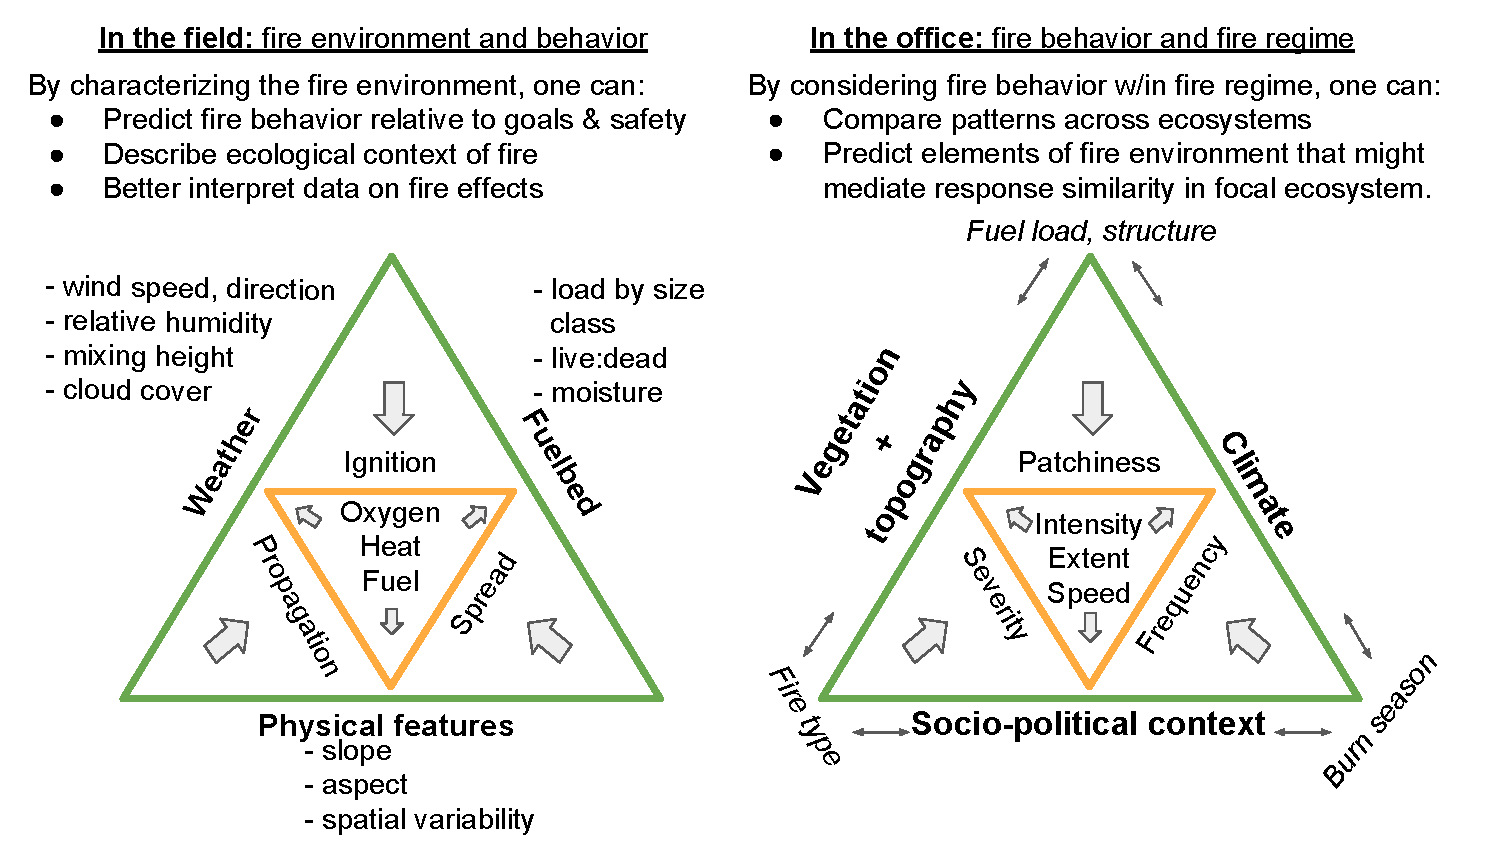
\includegraphics[width=1\textwidth]{WalletCard}
	\end{center}
	\caption{Two arenas of wildland fire science\textemdash the field and the office \citep{mcgranahan2018}. 
	This figure helps fire professionals from each arena identify characteristics of the fire environment or fire regime that dominate their colleagues' perspective.  
	\label{fig:WalletCard} }  %(Fig.~\ref{fig:WalletCard})
\end{figure}

This workshop has been designed to develop wildland fire science literacy by increasing the range of things fire professionals ``know something about'' when it comes to prescribed fire science and management. 
We hope that those who study prescribed fire have a better appreciation for what goes in to conducting an operation safely and effectively, and start to get some ideas on how to conduct better science in the management context.  
We hope that those who aim to use fire research have a more critical eye for what constitutes useful knowledge, in terms of both best practices in the science and transferability across management areas. 
And we hope that those who manage prescribed fire directly develop their critical thinking skills in assessing the \emph{what}, \emph{why}, and \emph{how} of burning as part of an ecological disturbance regime, and aim for more than just turning acres black. 


%
%	TOC
% 	
\newgeometry{textwidth=15cm}
	\tableofcontents
\restoregeometry
%
%	Call the sections
%
\part{Prescribed fire science}
	\chapter{Fire science basics}

In a given year, about 3\% of Earth's terrestrial surface burns \citep{archibald2018}.
All this fire affects air quality, alters vegetation, and drives processes such as climate and nutrient cycles \citep{sullivan2012}. 
A basic understanding of how fire burns is important for anyone involved in wildland fire science and management. 
The first part of this chapter introduces the processes of combustion, heat transfer, and fire spread.
The second part introduces some basics of how scientists measure and describe wildland fire. 

\section{Fire in space and time}

When conducting any type of fire science, one must be aware of multiple spatial and temporal scales at once. 
It is important to consider individual fires within the broader context of biogeography and climate, as well as consider the location of individual sample points within the landscape context of the individual fire. 
Thoughtful placement and timing\textemdash spatial and temporal considerations, respectively\textemdash of samples helps data from one fire fit into knowledge of many fires. 

\begin{figure}
	\begin{center}
		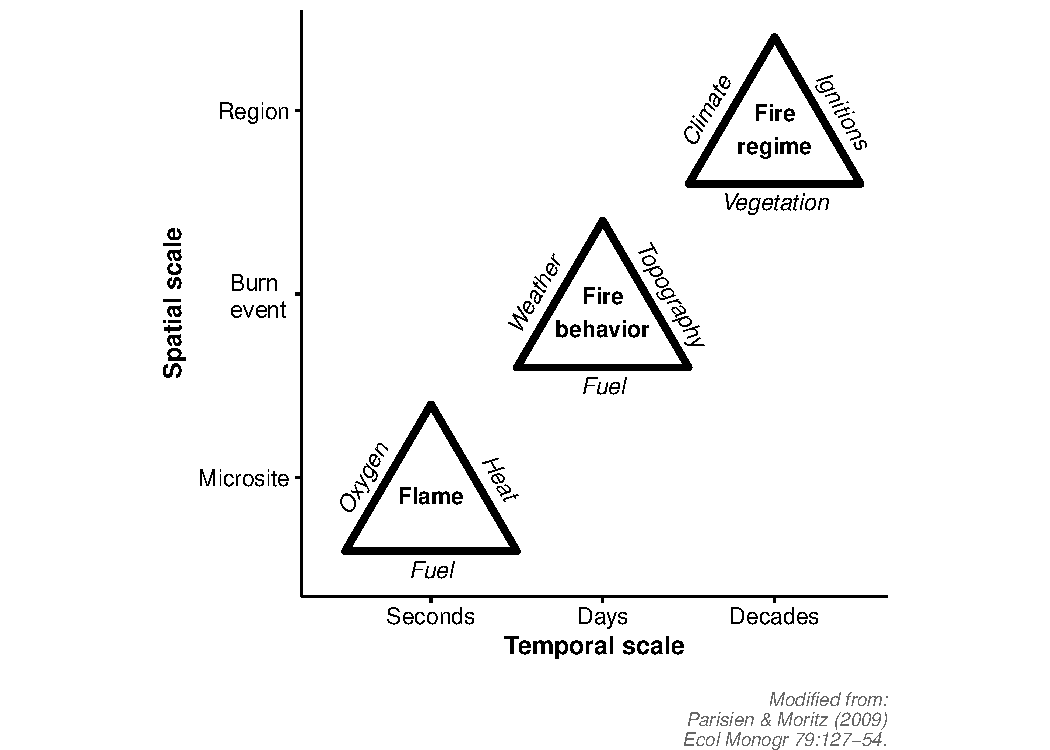
\includegraphics[width=1\columnwidth, 
		trim={2.75cm 1.5cm 2cm 0.5cm}, clip=true]
		{science/FlameTriangles-1}
		%(Fig.~\ref{fig:FireTriangles})
	\end{center}
	\caption{Three scales of wildland fire. Modified from \citet{parisien2009}.
		\label{fig:FireTriangles}}
\end{figure}

The story of fire in a landscape unfolds at three spatio-temporal scales (Fig.~\ref{fig:FireTriangles}). 
Each scale is relevant to the fire scientist. 
The finest and fastest scale is that of individual flames and the movement of the \emph{flaming front}, the series of ignitions that propagate fire through the fuelbed, and across the landscape. 

In prescribed fire, most personnel and planning focus on the middle triangle\textemdash the factors that affect how a fire behaves within the defined burn unit within the operational time period (often less than 1 day). 
How wind, topography, and fuel affect fire behavior is discussed in detail in the fire behavior chapter. 

Good fire management bases broad objectives within a model \emph{fire regime}, which is discussed in more detail later in this chapter. 
Within a given climate and vegetation type (e.g., grassland, savanna, or forest), managers often have fairly specific goals they desire to achieve, and various elements of prescribed fire can be manipulated to serve those goals. 
For example, both the season in which a burn occurs and the ignition pattern used to set it can affect the intensity of the prescribed fire. 
But burns in different seasons can target plants at different stages in their life cycles, as well, so clearly these two elements of the fire regime have important interactions in determining the ultimate effects of a single fire, and especially over time, if fires are repeated. 
Collecting quality data from the fire environment before and during a fire can provide a lot of information to fire managers about what their burns are doing, and how to better plan future operations to increase their chances to achieve their goals. 

\section{What is fire?}

All fire results from the combination of the three fundamental components of the Flame Triangle: Fuel, heat, and oxygen (Fig.~\ref{fig:FireTriangles}).
In the wildland fire environment, fuel consists of plant material. 
The ambient air provides oxygen.
Wind can increase oxygen input, while physical barriers can block air flow. 
Heat must come from an ignition such as lightning or an incendiary device, or from an already-burning fire nearby.

\subsection{Combustion} 

Combustion is a chemical reaction in which the rapid oxidation of plant material produces energy as heat:  

\begin{equation}\label{eq:combustion}
	(C_{6}H_{10}O_{5})_{n} + O_{2} + \text{energy}_{\substack{kindling\\temperature}} \rightarrow   CO_{2} + H_{2}O + \text{energy}_{heat}
\end{equation} 

The left-hand side of Eq.~\ref{eq:combustion} is simply the three components of the flame triangle in Fig.~\ref{fig:FireTriangles}: 

\begin{itemize}
	\item $C_{6}H_{10}O_{5}$ is the chemical formula for cellulose, which represents plant material as fuel. 
	\item Oxygen $O_{2}$ comes from the air. 
	\item \emph{Kindling temperature} is what fuel must be heated to before it ignites and combustion proceeds as a self-sustaining reaction (\~500\degC).
\end{itemize}

Note that in this format, combustion is the reverse of \emph{photosynthesis}, the processes that assembled the plant material in the first place:

\begin{equation}\label{eq:photosynthesis}
	CO_{2} + H_{2}O + \text{energy}_{solar} \rightarrow (C_{6}H_{10}O_{5})_{n} + O_{2}
\end{equation}

Thus, burning plant biomass\textemdash i.e., \emph{combustion}, Eq.~\ref{eq:combustion}\textemdash is just a natural decomposition process that breaks down vegetation. 

Combustion can be divided into distinct phases:\footnote{It is important to keep in mind that \textit{combustion in the wildland environment is not linear}. 
	Because vegetation has all sorts of sizes, arrangements, and chemical and moisture contents, wildland fuel particles heat unevenly and release gases and energy at different rates \citep{sullivan2012, finney2013}.
	In fact, fire ecologists have used an overly-simple model of combustion for decades \citep{sullivan2017}, which often focuses on changes in temperature.
	But combustion is better understood as the exchange of energy between the environment and plant matter at the surface of fuel particles, known as the \emph{reaction zone}. 
	These review papers really get into the complexities of wildland fuel combustion: \citep{sullivan2012, sullivan2017, sullivan2017a}.  
} 

\begin{enumerate} 
	\item \textbf{Preheating\textemdash}Fuel particles begin to absorb heat. Dehydration begins at 100\degC\textemdash moisture is driven out of fuel particles. This is an \emph{endothermic} part of the process, meaning it depends on heat from an external source. Often the energy source is an approaching flame front, so the heating rate increases as the flame front approaches. Flame contact leads to rapid heating. 
	\item \textbf{Pyrolysis\textemdash}The thermal degradation of matter. Around 200\degC, chemical bonds in the fuel start to break down. The fuel particle begins to lose mass as previously solid components like cellulose volatilize. Around 500\degC, any remaining material essentially turns into charcoal. 
	\item \textbf{Ignition\textemdash}The endothermic reaction that required heat input transitions to an \emph{exothermic} reaction that releases heat. More than just reaching a threshold temperature (e.g., \emph{kindling temperature}, as in Eq.~\ref{eq:combustion}), this phase means the reaction is releasing energy faster than the surrounding environment can absorb it.
	\item \textbf{Flaming combustion\textemdash}The reaction zone\textemdash the surface of the fuel particle between 200\textendash 500\degC\textemdash is engulfed in flame as the heated gases released by pyrolysis mix with oxygen in the air and ignite.
	\item \textbf{Glowing combustion\textemdash}Remainder of solid fuel particles continue to break down, even after all the gases have been released and burnt off as flames. Also known as \emph{smoldering}. 
	\item \textbf{Extinction\textemdash}Combustion finally ceases, but not necessarily because all of the fuel is gone. Once the reaction no longer produces energy faster than it can be absorbed by any moisture or inorganic materials nearby, the reaction will slow and the fuel particle will cool enough to stop combustion if no more energy is added. 
\end{enumerate}

\subsection{Heat transfer}

	\index{Heat transfer|textbf}
No matter how hot a fuel particle burns, wildland fire cannot spread unless heat energy transfers to another fuel particle. 
The transfer of heat energy from combusting fuel to adjacent particles is called \emph{propagation}. 
Heat transfer in the wildland fire environment follows three standard physical processes (Fig.~\ref{fig:HeatTransfer}): 
	\index{Propagation|textbf}

\begin{figure}
	\caption{
		The three basic mechanisms of heat transfer. Convection is often the most important mechanism in wildland fire: buoyant hot air moves uphill or is pushed ahead of the fire by wind to preheat fuels prior to contact with flames. 		  
		\label{fig:HeatTransfer} }
	\begin{center}
		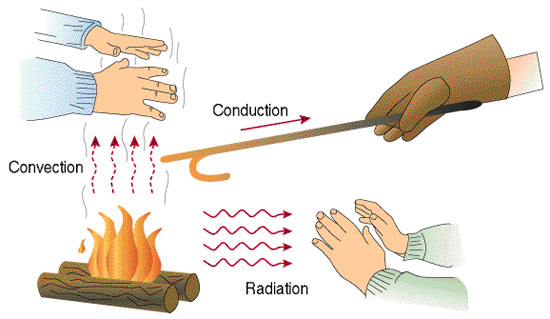
\includegraphics[width=1\textwidth, trim={0cm 0cm 0cm 0cm}, clip=true]{science/HeatTransfer}
			\ImageCredit{Kmecfiunit CC BY-SA 4.0}
			\ImageIndex{CC BY-SA 4.0}
		{fig:HeatTransfer}
		{Kmecfiunit}
		{https://upload.wikimedia.org/wikipedia/commons/e/e6/Heat-transmittance-means1.jpg}
		%(Fig.~\ref{fig:HeatTransfer})
	\end{center}
\end{figure}

\begin{itemize}
	\item \textbf{Conduction\textemdash}The transfer of heat through direct contact, from molecule to molecule within an object. Since plant matter generally conducts heat poorly, especially when dry, conduction in the wildland fire environment is primarily limited to carrying heat through soil and large-diameter fuels like logs. 
	\item \textbf{Convection\textemdash}The transfer of heat through air flow is important in determining the direction of fire spread.\footnote{As further evidence of the complexity of the wildland fire environment, convection can also \emph{cool} fuel particles that are being heated by other processes, and the relative influence of heat loss vs. heat gain increases with the surface area:volume ratio of the fuel particle \citep{finney2013}.} \emph{Free convection} is the buoyant rise of heated air; \emph{forced convection} is hot air moved by wind.
	\item \textbf{Radiation\textemdash}The transfer of energy via electromagnetic waves.While radiation can occur over relatively long distances, it requires unhindered line-of-sight movement and is thus limited to much shorter ranges in dense fuels. 
\end{itemize}

\begin{figure}
	\caption{
		Flame pulsation 		  
		\label{fig:FlamePulsation} }
	\begin{center}
		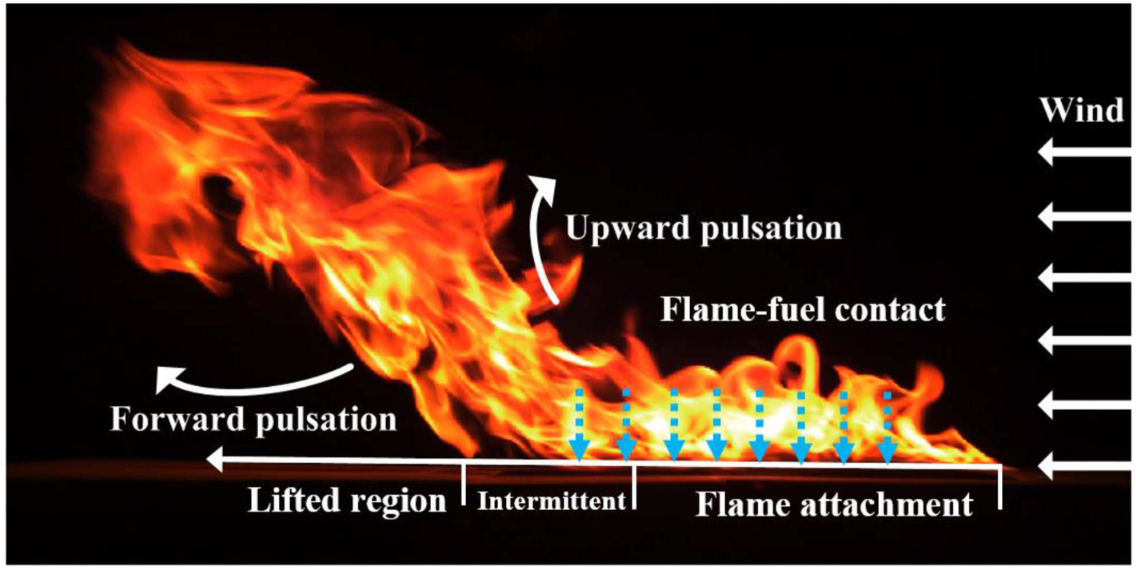
\includegraphics[width=1\textwidth, 
		trim={0cm 0cm 0cm 0cm}, clip=true]
		{science/FlamePulsation}
		\ImageCredit{\citet{tang2019}, CC BY 4.0}
		\ImageIndex{CC BY 4.0}
		{fig:FlamePulsation}
		{\citet{tang2019}}
		{https://www.frontiersin.org/articles/10.3389/fmech.2019.00034/full}
		%(Fig.~\ref{fig:FlamePulsation})
	\end{center}
\end{figure}

Two other heat transfer mechanisms are also important in the wildland fire environment:

\begin{itemize}
	\item \textbf{Direct flame contact} is critical to propagation as it can ignite particles ahead of the flame front (Fig.~\ref{fig:FlamePulsation}). Flames can be pushed forward by wind, or even by a fire's own fluid dynamics. 
	Brief, fine-scale turbulent pulsations created by fresh air flowing into the reaction zone as buoyant hot air lifts away can create horizontal vortices that push flames down, into contact with pre-heated fuel particles. The flame contact rapidly bringing them up to ignition temperature.\footnote{\citet{finney2015, tang2017, morandini2018}} 
	\item \textbf{Solid fuel transport} is the physical movement and deposition of burning fuel particles: 
	\begin{itemize}
		\item Large burning particles can break apart as pyrolysis degrades them; these burning chunks can fall or roll and cause ignition downhill.
		\item \emph{Firebrands}, or burning embers, can get carried by wind and fall far from the original fire. When firebrands land in a receptive fuelbed that is dry enough to ignite, they start \emph{spot fires}.
	\end{itemize}
\end{itemize}

\section{Wildland fuels} 

	\index{Fuel!Fuel characteristics|textbf}
Wildland fuels are comprised of plant material. 
There are many species of plants, and they take many forms. 
Thus many properties describe wildland fuels: vegetation type (e.g., grasses, brush, coniferous or deciduous trees, logging slash, etc.); arrangement and structure (e.g., horizontal or vertical, continuous or discontinuous); particle size, along with surface area to volume ratio; particle density (loft, or packing ratio); whether the vegetation is alive or dead, standing or fallen, and whether it was derived from leaves or stems. 
But since fire spread depends on the transfer of heat energy through the environment, the diversity of plants can be functionally reduced to just a few categories of wildland fuel based on their thermal properties. 

\subsection{Fuel size classes} 

\index{Fuel!Fuel characteristics!Size classes|textbf}

\begin{marginfigure}
	\begin{center}
		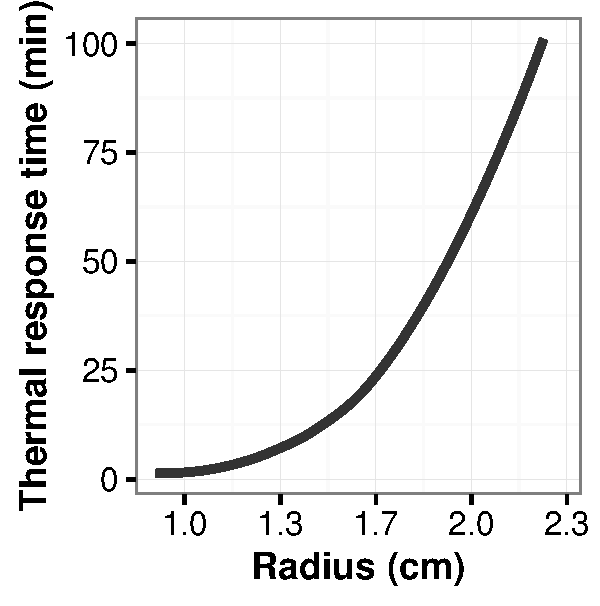
\includegraphics[width=1\textwidth, 
		trim={0cm 0cm 0cm 0},clip=true]
		{science/fosberg1973-1}
		\DataCredit{\citet{fosberg1973}}
		\caption{The non-linear relationship between fuel particle size and heat transfer rate.
			Small increases in fuel particle radius leads to disproportionately large increases in thermal response time\textemdash the speed at which the material changes temperature. 
			Thus, a fuel particle with radius 1 cm has a response time of 1.4 min, while  the response time jumps to 56 min for a particle of 2 cm radius. } \label{fig:Fosberg1973}
	\end{center}
\end{marginfigure} 

The primary categorization is \emph{size class}, which is given by a fuel particle's diameter.
Different diameters produce different surface area:volume ratios, which affects heat transfer rates: both how quickly the particle gains heat during pre-heating (Fig.~\ref{fig:Fosberg1973}), and the rate at which heat is lost while smoldering prior to extinction. 
Fuel size classes are referred to by their \emph{lag times}, which refers to how quickly fuel particles gain and lose heat and moisture.
The size classes of fuel are 1-hour, 10-hour, and 100-hour, which correspond to diameters of $<$ 0.6 cm,  0.6\textendash 2.5 cm, and 2.5\textendash 7.6 cm, respectively \citep{fosberg1971}.\footnote{The metric delineations might seem odd, but the original categories were in inches: $<$ 0.25, 0.25\textendash 1, 1\textendash 3. Some recognize a 1,000-hr class for very large fuels.}

It is often sufficient to differentiate fine fuel (1-hr) from coarse fuel (10-hr and above). 
Physically, fine fuels are ``thermally thin'', with low surface area:volume ratios that take on heat quickly and evenly, and have often fully combusted by the time the flame front passes. 
In the field, the fine/coarse distinction might apply to grasses vs. larger shrubs, trees, and downed woody debris.\footnote{
In prescribed fire, fine and coarse fuels are often managed separately\textemdash undesired woody plants might be targeted for heating, while desired species are to be protected, and keeping a pile of woody debris from igniting in the first place is the best way to ensure it doesn't kick up embers hours after everyone has gone home.}

\subsection{Fuel moisture}
\index{Fuel!Fuel moisture|textbf}

Fuel moisture is an important property, and wildland fuel moisture dynamics follow the size classes described above. 
\index{Fuel!Fuel types!Dead fuels}
\index{Fuel!Fuel types!Live fuels}
But first it is important to distinguish between living versus dead vegetation. 
There are two reasons fuels ought to be considered a class by themselves \citep{finney2013}:\sidenote{
	Fire scientists have struggled to account for live vegetation.
	In the parlance of wildland fire science, live fuels are often \emph{not available to burn} because they are insufficiently \emph{cured}, i.e. they haven't been dried out through exposure to warm air or radiation. 
	Because many management fires occur outside of dry, dormant seasons or in fuelbeds dominated by invasive species, prescribed fire managers (and scientists) must think beyond dead fuels alone. } 
\begin{itemize}
	\item Moisture in living plant tissue is under the biological control of the organism (ecophysiology), whereas dead fuel moisture is a passive interaction between plant tissue and the environment.
	\item Live tissue moisture often exceeds levels that will support combustion\textemdash in terms of heat flux, this moisture absorbs energy, making living plant tissue more of a sink than a source of combustion energy.
	And live tissues retain this moisture until their cells fail, slowing dehydration.  
\end{itemize}

\index{Lag times|see {Fuel characteristics, size classes}} 
\index{Fuel!Fuel characteristics!Size classes}
Within dead fuels, the concept of lag times applies to fuel moisture gain and loss as well as heating and cooling: dead fuel moisture depends on the moisture content of the air around it. 
All dead fuels passively gain and lose moisture by exposure to the atmosphere, and fine dead fuel moisture changes faster than coarse fuels. 

Several environmental variables affect fuel moisture transfer rates.
\index{Weather!Relative humidity}
\index{Weather!Precipitation}
Sources of moisture include the atmosphere itself\textemdash humidity and precipitation\textemdash and contact with other sources capable of holding and releasing moisture, such as soil and forest duff.
\index{Fuel!Fuel characteristics!Equilibrium moisture content}
\index{Equilibrium moisture content|see {Fuel characteristics}} 
When these sources are steady, fuel particles eventually reach an \emph{equilibrium moisture content} with the surrounding air\textemdash gains and losses of moisture via diffusion with the air are net neutral. 
Fine fuels reach equilibrium moisture content within a matter of hours, while coarse fuel can take days or weeks to become available for combustion if they got soaked through.
Drying increases with exposure to both wind and solar radiation \citep{byram1943}.

\subsection{The fuelbed and fire types}

\index{Fuel!Fuelbed|textbf} 
Wildland fuels occupy a three-dimensional space called the \emph{fuelbed} through which flame fronts spread from particle to particle. 
As such, the structure of plant biomass in this three-dimensional space has a major effect on fire. 
Within the landscape, the type of vegetation\textemdash grassland, brush, or forest\textemdash determines the type of fuel available to burn. 
Within the combustion reaction zone, the arrangement and density of fuel particles regulate the flame triangle\textemdash fuel availability, oxygen flow, and how quickly heat transfers to new fuel particles.  

\index{Fire types|textbf}
\index{Fire types!Ground fire}
\index{Fire types!Surface fire}
Three broad fire types are defined by the fuel layer through which fire spreads (Fig. \ref{fig:FireTypes}): \emph{ground fires} burn through organic material below the soil surface, such as peat and heavy forest duff; \emph{surface fires} burn through herbaceous and brushy aboveground plant biomass rooted in, or laying on, the soil surface; and \emph{canopy fires} burn through the foliage of standing trees; \emph{torching} is when the canopy of a single tree burns, while fire propagating from one canopy to another \emph{running crown fire}. 
Although fire rarely starts in the canopy, canopy fuels can be ignited by extremely high surface flames or via \emph{ladder fuels}\textemdash hanging branches, vines, or shrubs and trees of younger age classes that carry fire into the canopy after first being ignited on the surface. \index{Fuel!Fuel types!Ladder fuels} 
These canopy dynamics are a vivid illustration of the importance of \emph{horizontal continuity}\textemdash how far apart the trees are\textemdash and \emph{vertical continuity} between surface and canopy fuels, but these dynamics are at play in determining surface fire spread and behavior, as well.  

\begin{figure*}
	\begin{center}
		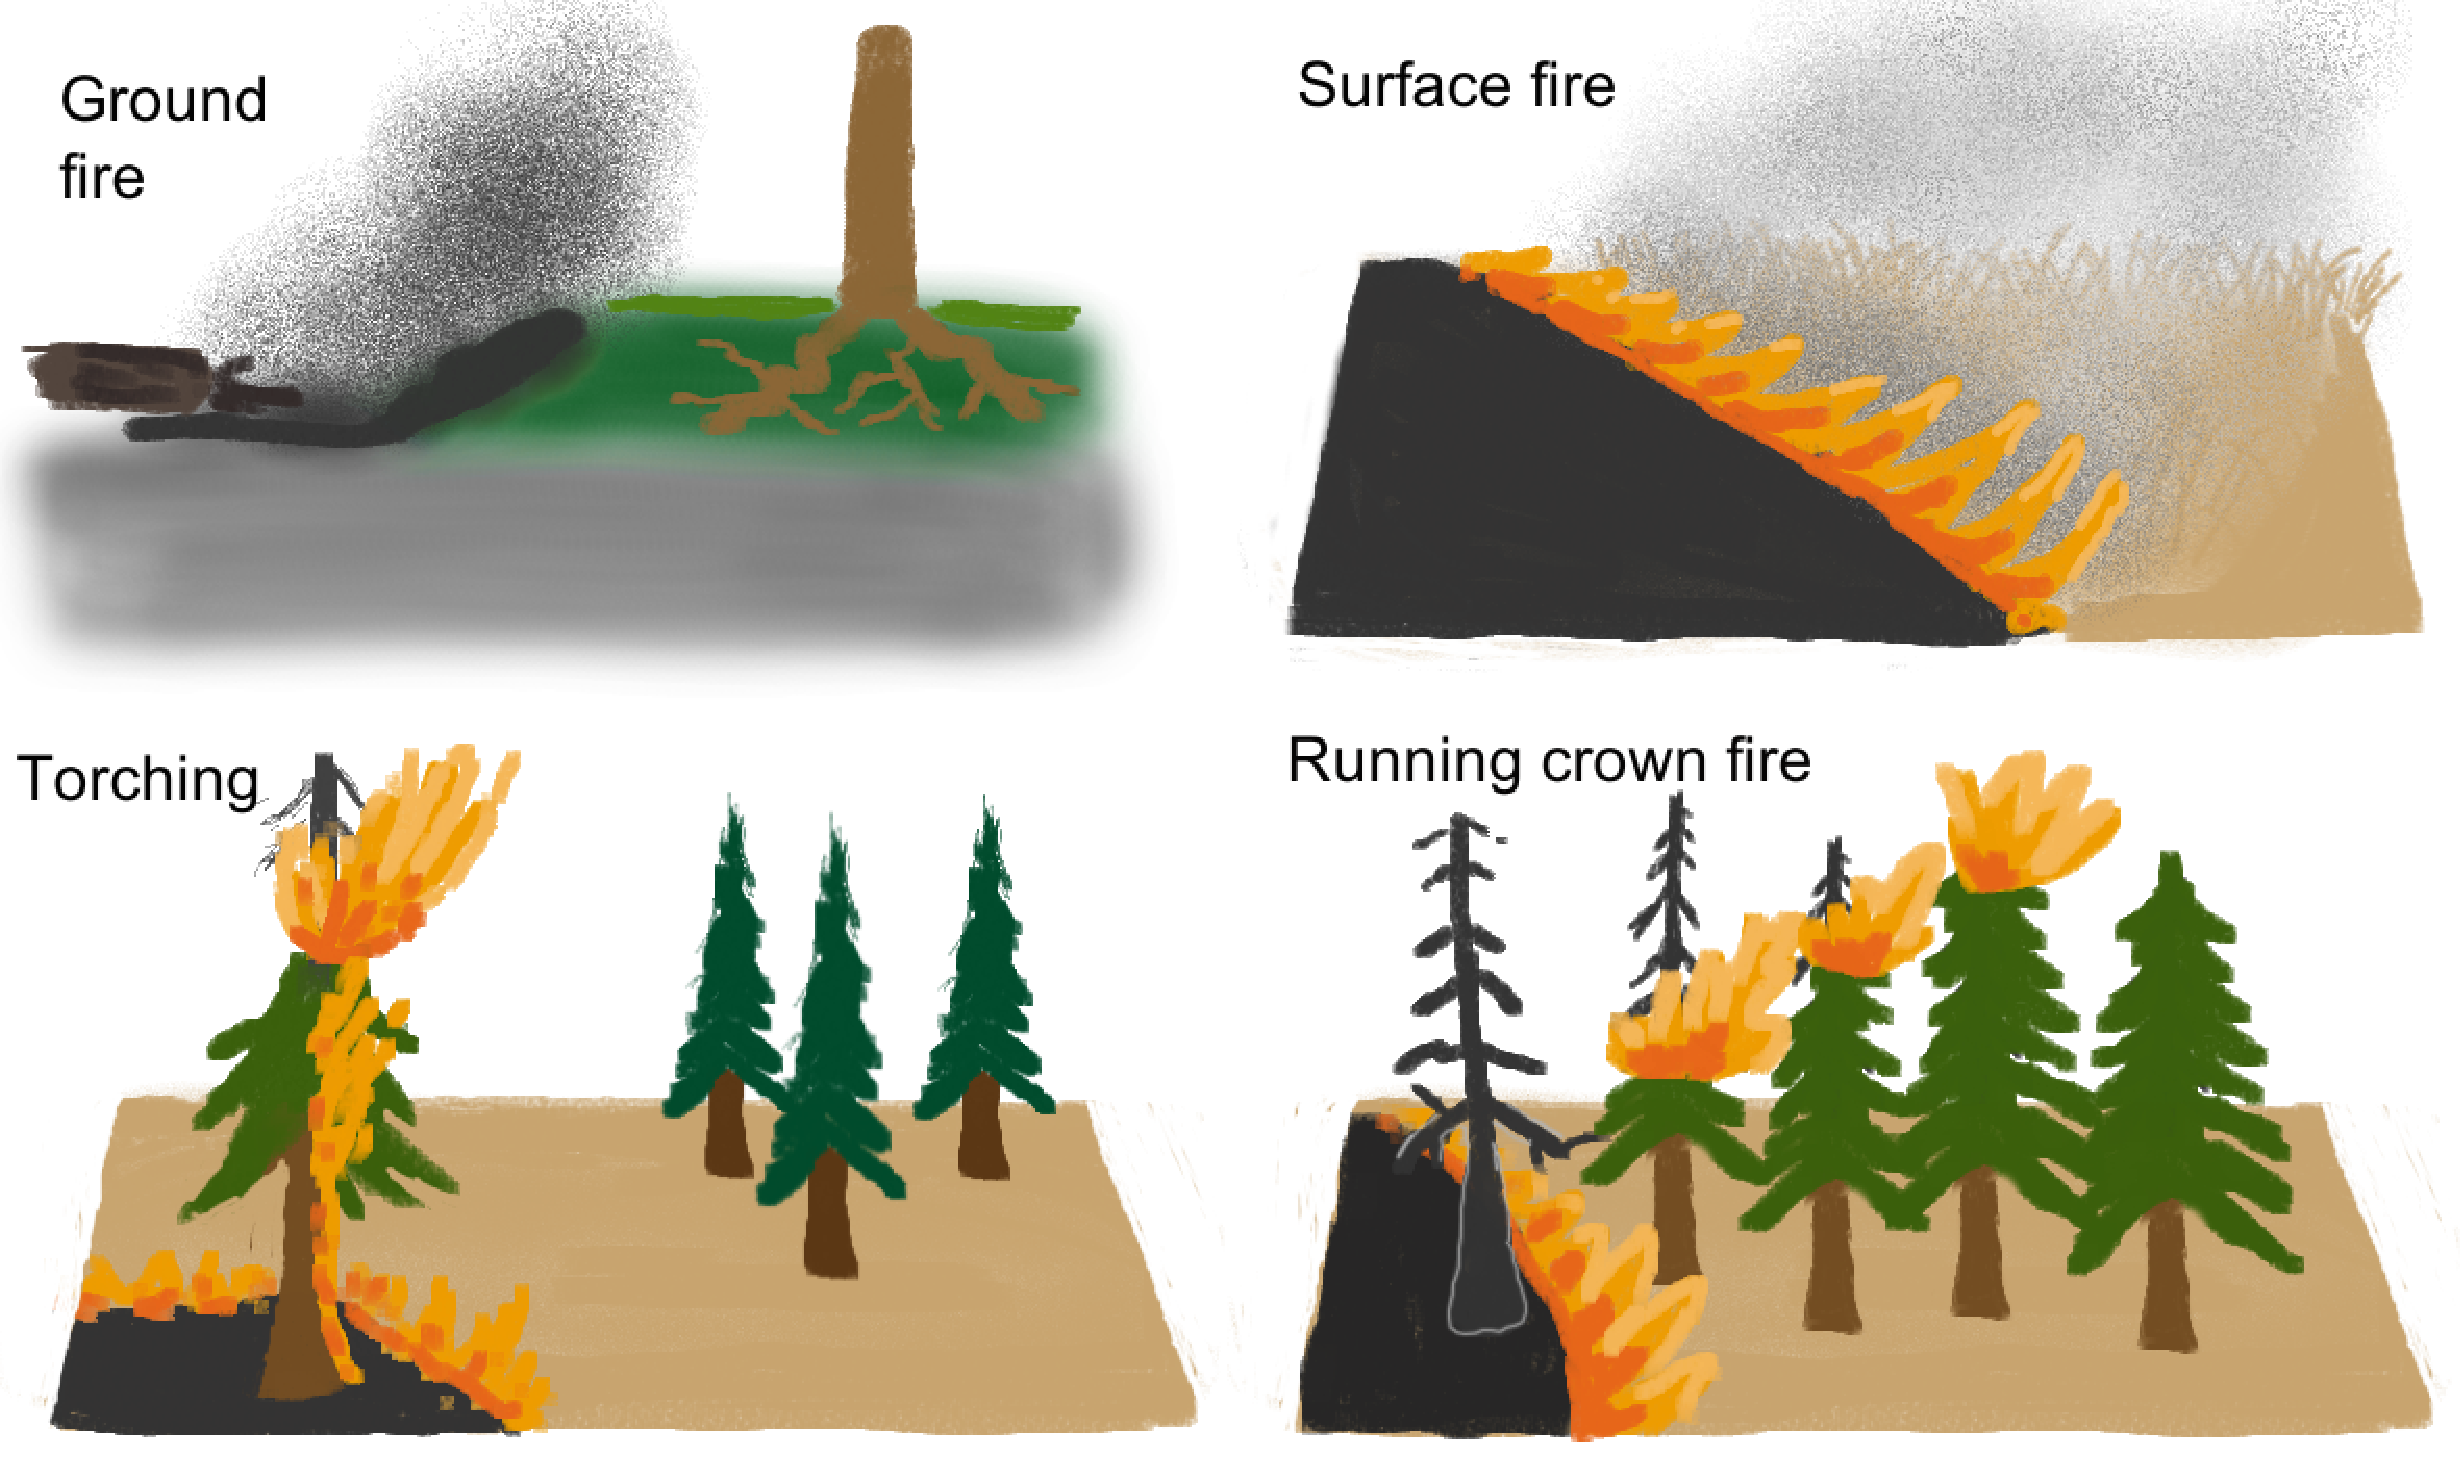
\includegraphics[width=1\textwidth]
		{science/FireTypes}
		%(Fig.~\ref{fig:FireTypes})
	\end{center}
	\caption{Four types of wildland fires. 
		\emph{Ground fires} burn underground through organic material like peat, while \emph{surface fires} move aboveground through fuels on the soil surface. 
		Fire can transition to tree canopies, as well. 
		\emph{Torching} occurs when the canopy of a single tree burns, while \emph{running crown fires} involve canopies of multiple trees.
		\label{fig:FireTypes}}
\end{figure*} 

\section{Fire behavior}

\index{Fire behavior|textbf}
\emph{Fire behavior} describes energy release by the combustion of vegetation, and is controlled by the three factors in the Fire Behavior Triangle  (Fig.~\ref{fig:FireBehaviorTriangle}).  
With knowledge and experience, wildland fire professionals can learn to anticipate how environmental factors influence fire behavior in a particular fuelbed.

Direct observations include how fast a fire moves, how long fuels burn, and the length of flames. 
Indirect observations include how much unburned fuel is left behind, or how high up trees are scorched by flames.

Two standard descriptors of fire behavior are rate of spread and intensity.
\emph{Rate of spread} is simply how fast the flame front moves through the fuelbed.
\emph{Intensity}\textemdash which is not directly observable \textemdash refers to energy release; specifically, \emph{fireline intensity} is the amount of heat released per length of flame front within a period of time \citep{rothermel1983}.
\index{Fire behaviour!Flame length}
\emph{Flame length} is directly related to the rate of energy release and thus serves as an observable proxy of intensity \citep{rothermel1983}.
Both fireline intensity and flame length increase with fuel load and decrease as fuel moisture increases \citep{kreye2013}.

\begin{marginfigure}
	\begin{center}
		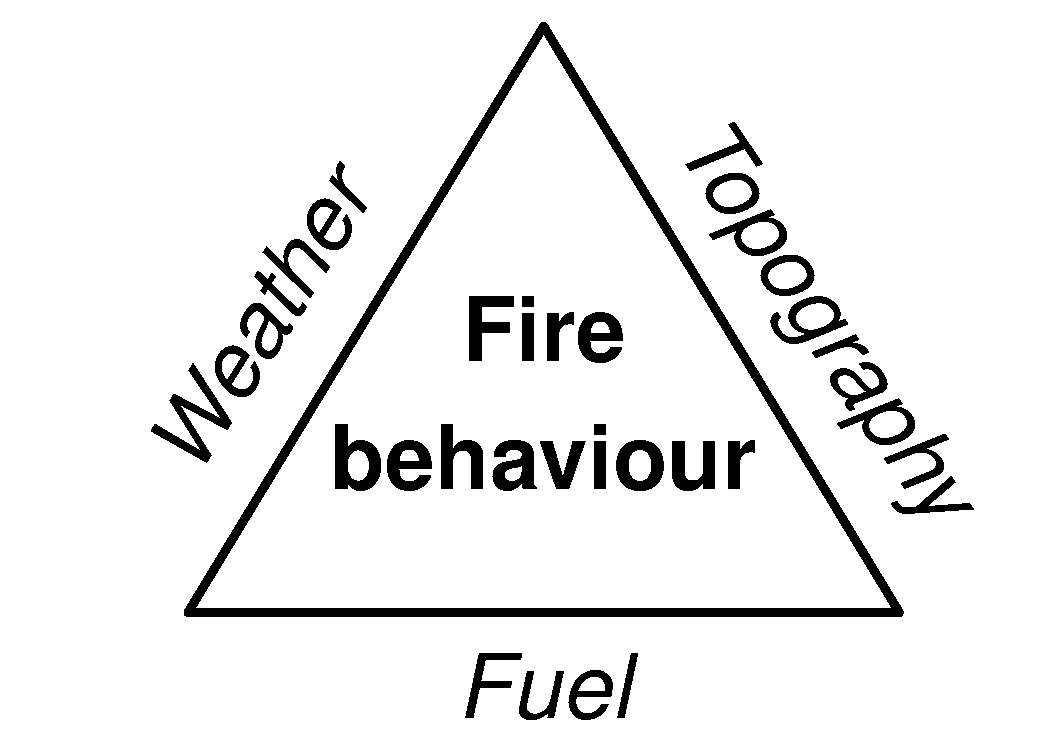
\includegraphics[width=2.2in, 
		trim={1.5cm 0cm 1cm 0.5cm}, clip=true]
		{science/behavior/FireBehaviourTriangle-1}
		\caption{Topography, weather, and the fuelbed are the three major drivers of wildland fire behavior.
			\index{Fire triangles!Fire behavior|textit} \label{fig:FireBehaviorTriangle} } 
		% (Fig.~\ref{fig:FireBehaviorTriangle})
	\end{center}
\end{marginfigure}

When fuels are constant, variability in fire behavior is driven primarily by wind and the flatness or steepness of the terrain, or \emph{slope}. 
Wind and slope are important because they affect heat transfer and facilitate pre-heating, which is the critical mechanism for flame propagation \citep{sancheztarifa1967}. 
Wind pushes heat ahead of the flame front and hot air rises upslope, both of which increase convective heat transfer \citep{sharples2008}.
\index{Heat transfer!Convection} 
\index{Heat transfer!Flames}
Both also reduce the angle between the flame and surface fuels, increasing the probability of heat transfer via flame contact.
The effect is for fires to move faster with the wind, or up a slope, and more slowly against the wind, or down a slope, than in the absence of either.

\section{Wildland fire anatomy} 

	\index{Fuel!Fuelbed}
Because the effects of slope and wind on heat transfer are predictable, one can also predict the shape and direction of wildland fire spread through a given fuelbed.
Fire behavior also varies predictably at different points along the fire perimeter relative to wind direction and slope. 

Assume a single-point ignition in a flat grass fuelbed. 
Without wind, the flame front would slowly spread at a constant rate in all directions. 
Heat transfer is limited to particles very near the reaction zone. 
A fire under a no-wind scenario appears as a slowly-expanding circle. 
But if a wind were to rise, heat transfer rates will vary between the upwind and downwind directions and the shape of the fire becomes elliptical as different parts of the fire spread at different rates (Fig.~\ref{fig:EllipseCartoon}). 

\begin{figure}
	\caption{The anatomy of a surface fire. 
		Here the wind moves from left to right, giving the fire an elliptical shape as the \emph{heading fire} moves fastest with the wind, and has the longest flames. 
		Conversely, the \emph{backing fire} moves the slowest, creeping into the wind. 
		On each side, \emph{flanking fires} spread perpendicular to the wind at a rate between the backing and heading fires; they are aerated by the wind but are neither moving fully against it nor with it. 
		The burned area in the center of the fire is often called ``the black'' and is an important safety zone for fire personnel due to the lack of remaining fuel. 
		The spot fire was ignited by a \emph{firebrand}, or ember, carried ahead of the main fire by the wind. 
		\label{fig:EllipseCartoon}  }
	\begin{center}
		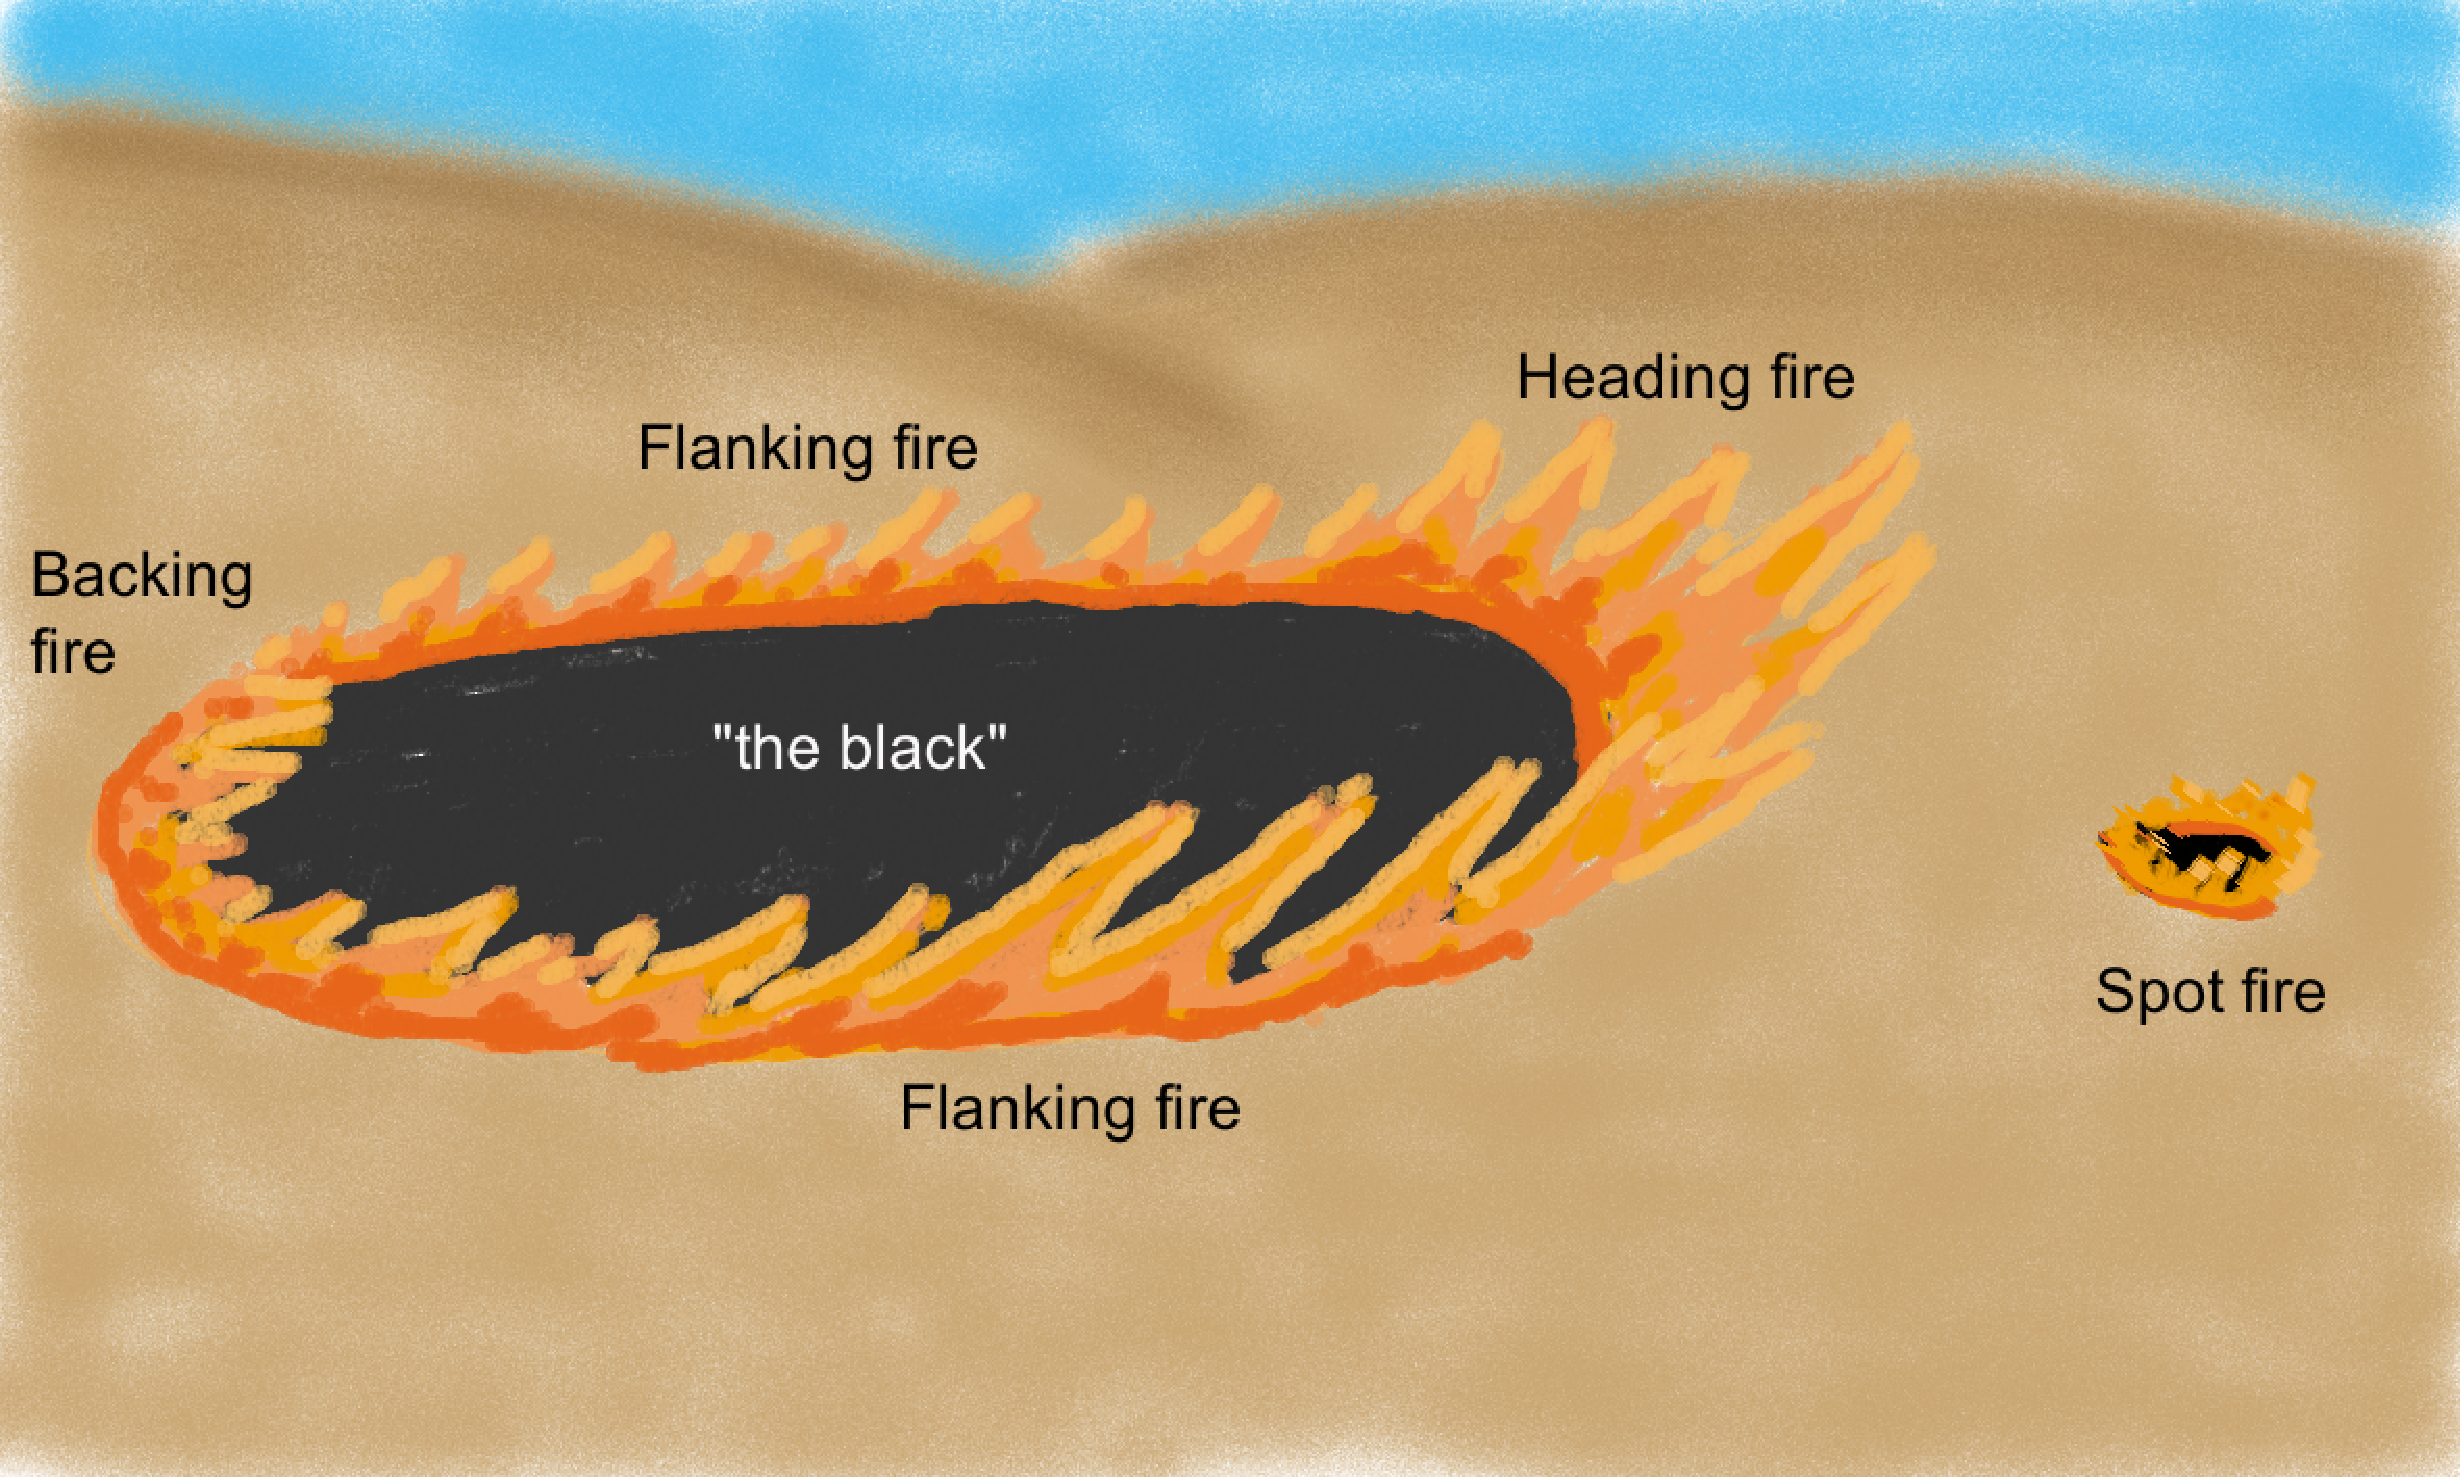
\includegraphics[width=1\textwidth, 
		trim={0cm 3cm 0cm 0cm}, clip=true]
		{science/FireAnatomy}
		%(Fig. \ref{fig:EllipseCartoon})
	\end{center}
\end{figure}

While fire \emph{spreads} outward as a flame front via propagation, \emph{fire growth} is driven by increases in burned area, including the spot fires that accelerate the increase in burned area beyond the spread of individual flame fronts.
On level terrain with a continuous, even fuelbed and constant wind, the shape of a fire's burned area depends primarily on wind speed.
The higher the wind speed, the longer and more narrow the burn perimeter.

A brief description of the anatomy of a wildland fire:

\begin{marginfigure}
	\begin{center}
		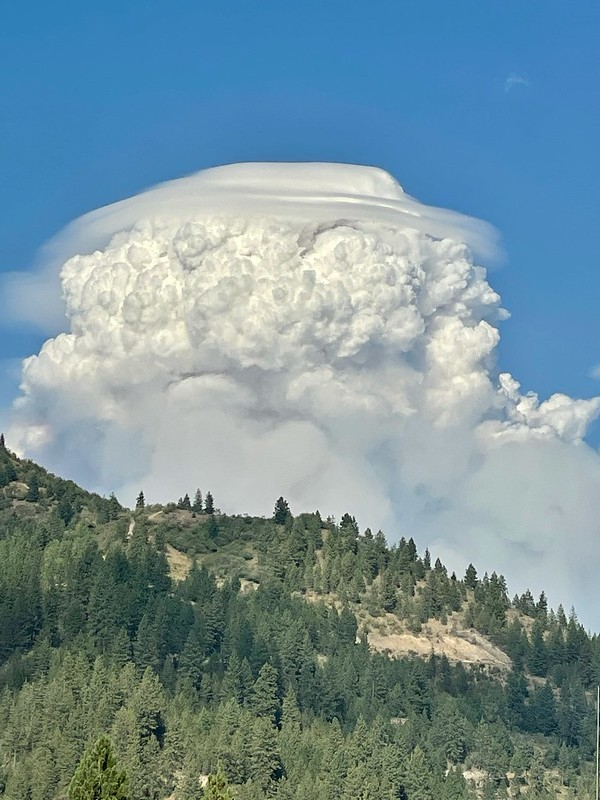
\includegraphics[width=1\textwidth, 
		                trim={0 0cm 0 0},clip=true]
		        {science/VeryLargePlume}
	% 	\PhotoCredit{ }
		\caption{Such a large smoke plume has developed over this wildfire that it has altered cloud formation at its top, several thousand feet above the fire.} 
		\label{fig:BigPlume} %(Fig.~\ref{fig:BigPlume})
	\end{center}
\end{marginfigure} 

\begin{itemize}[noitemsep]
	\item \textbf{Head(ing) fires} move with the wind. 
Wind drives convective heat transfer by pushing warm air ahead of the fire,  which accelerates pre-heating, propagation, and fire spread.
\item \textbf{Backing fires} crawl into the wind. 
Blowing heat back over previously burned areas instead of into unburned fuel reduces preheating.
\item \textbf{Flanking fires} are the sides of the fire that burn parallel to the wind.
The lower intensity of flanking fires can be important tactically for wildland firefighters, as it is easier to fight these flames directly and work toward the head fire, reducing the total area burned.\footnote[][1cm]{Because a wind shift could easily turn a flanking fire into a head fire, it is important that personnel working on a flanking fire do so from the burned area within the perimeter, which serves as a safety zone.} 
\item \textbf{Spot fires} start via \emph{firebrands}\textemdash burning embers carried ahead of a flame front by wind or convection.
\item The \textbf{smoke plume} consists of the ``gases, smoke, and debris that rise slowly from a fire while being carried along the ground because the buoyant forces are exceeded by those of the ambient surface wind \citep{nwcg2019}.'' 
Plumes that develop strong updraft are called \emph{convective columns}, highlighting their effect on fire behavior (Fig.~\ref{fig:BigPlume}). 
Many fire-atmosphere interactions that relate to convective lift aren't directly visible. 
Plume structure provides insight into atmospheric conditions and plume properties such as color and roiling indicate fire behavior. 
\end{itemize} 

\subsection{Fire-atmosphere interactions}

Fires interact with the atmosphere. 
Crucially, these interactions are often simultaneously the least visible factors affecting fire behavior and the most important factors affecting the safety and effectiveness of prescribed burns. 
Thus it is important for all prescribed fire professionals to know how to read the signs that indicate how a fire is interacting with the invisible atmosphere. 

\begin{figure*}
	\caption{An illustration of general indicators of \emph{atmospheric stability}\textemdash the resistance of the atmosphere to mixing via vertical movement of air. 
		A stable atmosphere  resists mixing, which limits convective lift of smoke and generally subdues fire behavior. 
		An unstable atmosphere is receptive to rapid convection and smoke lift, which increases ventilation of the combustion reaction zone and increases fire intensity. 
		\label{fig:AtmopshericStability}  }
	\begin{center}
		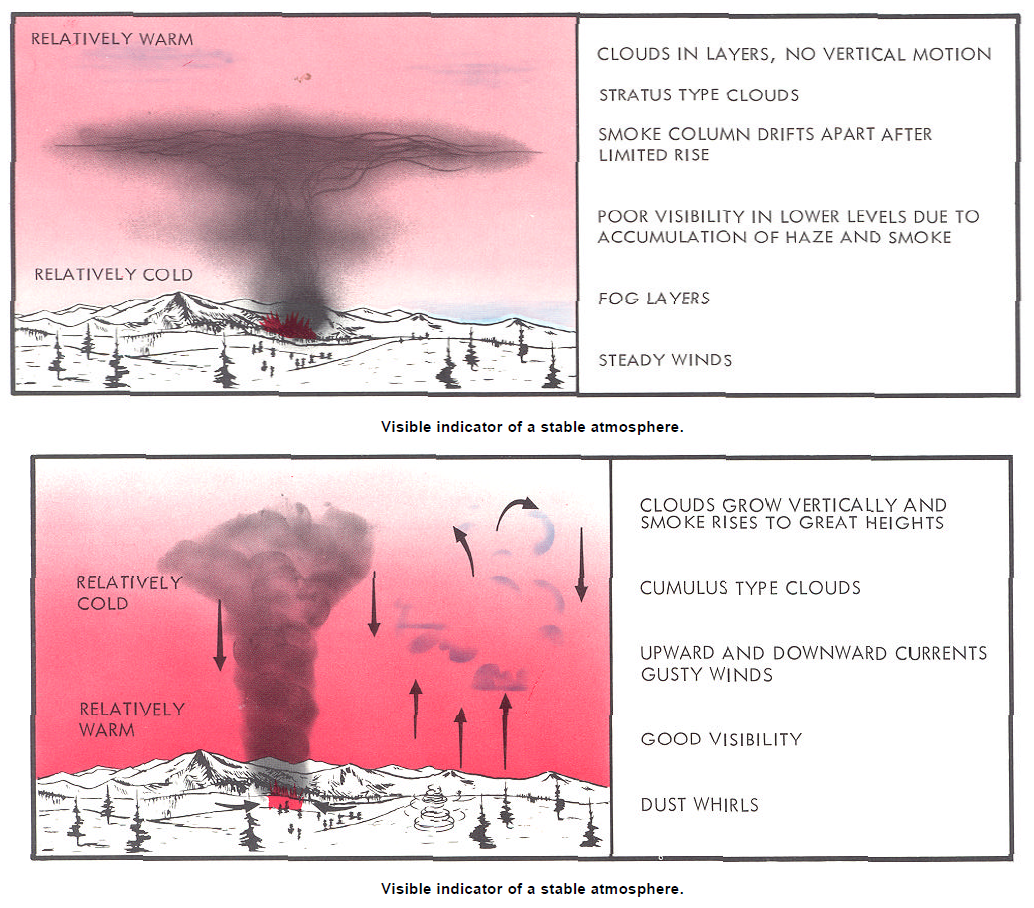
\includegraphics[width=1\textwidth, 
		trim={0cm 0cm 0cm 0cm}, clip=true]
		{science/AtmosphericStability}
		%(Fig. \ref{fig:AtmopshericStability})
			\ImageCredit{\citet{schroeder1970}}
	\end{center}
\end{figure*}

	\index{Atmosphere!Atmospheric stability} 
\emph{Atmospheric stability} refers to how resistant the atmosphere is to vertical air movement, one of the controls on fire behavior \citep[][Fig. \ref{fig:AtmopshericStability})]{schroeder1970}. 
Hot combustion gasses and heated air are buoyant, and naturally seek to rise until the air expands and cools. 
In an unstable atmosphere, warm air rises easily, which increases convective airflow away from the combustion zone.
One cannot directly observe instability, but meteorologists can measure and predict associated variables. 
US fire weather forecasts include the \emph{Haines Index}, an index of the potential for rapid fire growth derived from correlations between observed fire behaviour and atmospheric stability \citep{haines1988}.
	\index{Haines Index}   
	
An \emph{inversion} is a departure from the typical pattern in which air gets colder with distance from the Earth's surface. 
\emph{Surface inversions} are deep layers of cool air near the surface, also known as \emph{night inversions} because such cooling often occurs at night \citep{schroeder1970}. 
Inversions form low, stable barriers of air that prevent mixing, convection, and smoke dispersal. 
Although inversions are prominent in mountainous regions, night inversions often form over broad areas without topography. 

The effect of an inversion on fire behavior is sometimes most noticeable as the inversion lifts.
By suppressing convection, inversions have the obvious effect of reducing the intensity of wildland fire burning under it, perhaps a prescribed fire lit during the morning. 
But as solar heating in the morning warms the surface, warm air begins to circulate in the near-surface atmosphere and starts to mix with higher layers. 
This convection and mixing weakens the inversion until it lifts entirely, allowing convective currents to reach to the top of the \emph{troposphere}, the lowest layer of the atmosphere that interacts with the Earth's surface. 
The consequence for fire behavior is greater intensity as convection develops.
 
\section{The fire regime} 

The fire regime of an area is the product of climate, vegetation, and the pattern of ignitions averaged over a given period of time (Fig.~\ref{fig:RegimeTriangle}). 
Many of the specific parameters of fire regimes\textemdash fire frequency, spatial extent, seasonality, intensity, and fire type\textemdash can also describe individual fire events. 

\begin{marginfigure}
	\begin{center}
		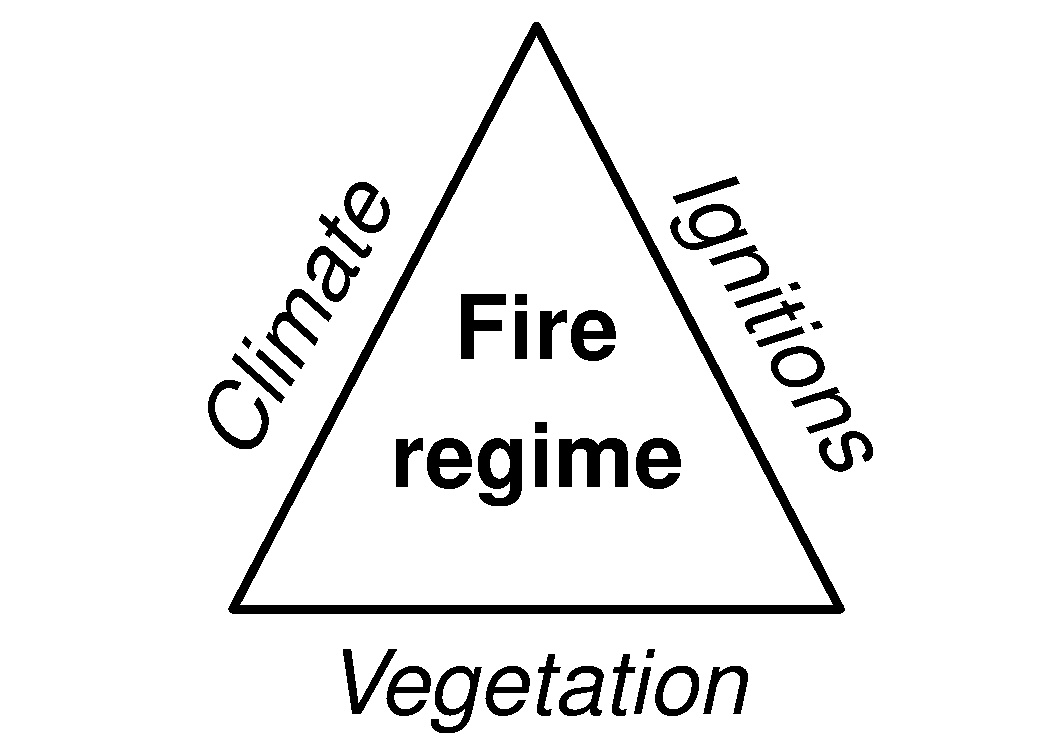
\includegraphics[width=2.2in, 
		trim={3cm 0cm 3cm 0},clip=true]
		{science/FireRegimeTriangle-1}
		\caption{The three sides of the Fire Regime Triangle.
			See Fig.~\ref{fig:ParametersFactors} for specific components with each side of the triangle.  }
		\index{Fire triangles!Fire regime|textit}
		\label{fig:RegimeTriangle} 	% (Fig.~\ref{fig:RegimeTriangle})
	\end{center}
\end{marginfigure} 

While the term \emph{fire regime} typically refers to a ``core group of parameters describing which fires occur when and where according to frequency, size, seasonality, intensity, and type'' \citep[][p. 61]{krebs2010}, many parameters are a product of two or more sides of the Fire Regime Triangle and are controlled at multiple temporal scales.

The importance of the fire regime concept to wildland fire science and management can hardly be overstated. 
The fire regime concept underpins the objectives of fire management policy as well as the strategy and tactics of prescribed fire operations (Fig.~\ref{fig:WalletCard}). 
Thus, to be useful, wildland fire scientists must target data collection to measure components of the wildland fire environment that relate to the targeted components of the fire regime.
Let us focus on the \emph{core parameters} of fire regime\textemdash the physical parameters of a specific fire, or the typical fire in an area. 

\begin{figure*} 
	%	\begin{center}
	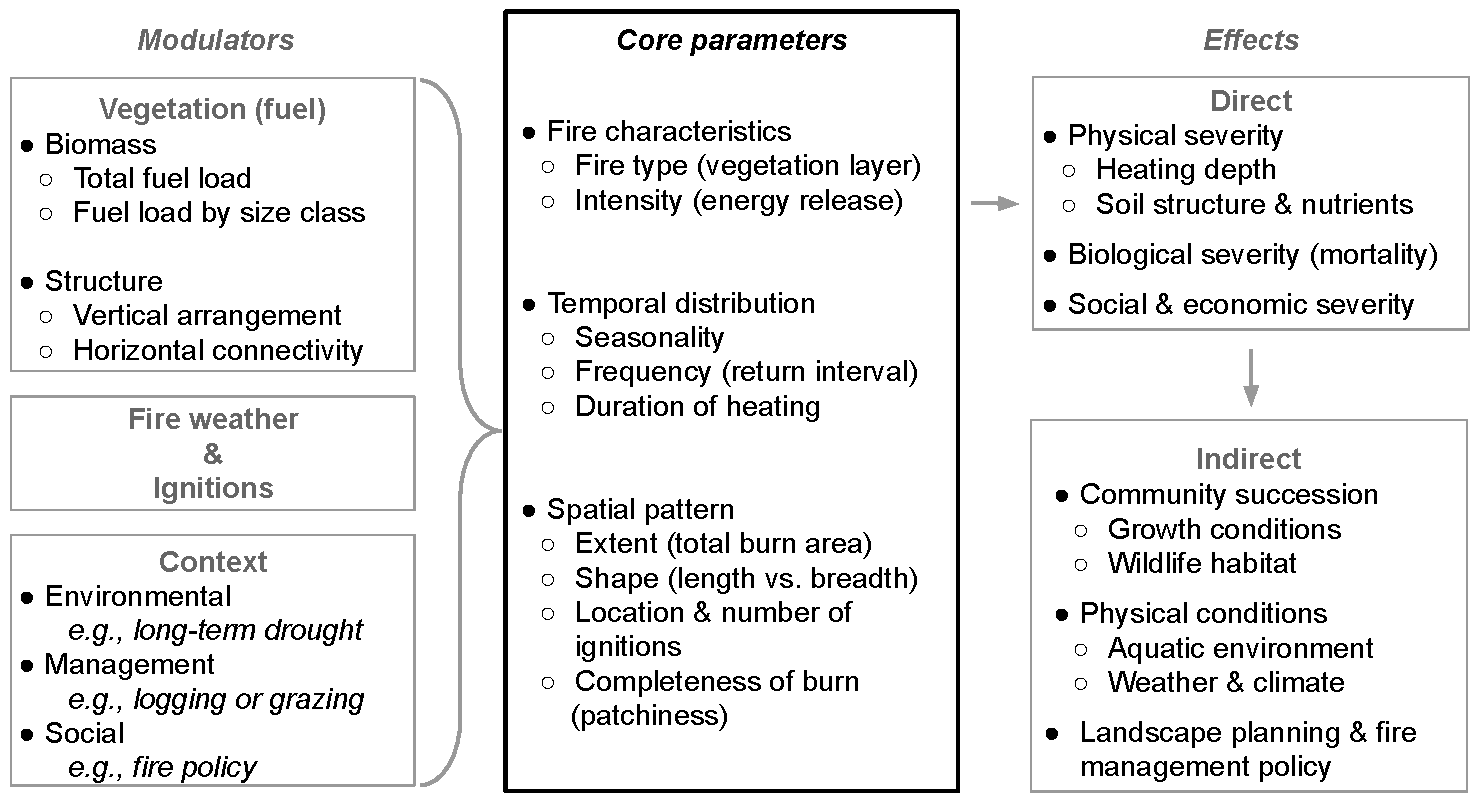
\includegraphics[width=0.85\paperwidth]
	{science/FireRegimeParts}
	\caption{
		The fire regime concept can be divided into core parameters\textemdash those that describe the physical characteristics of either one fire event, or the typical fire event\textemdash as well as biological, meteorological, and social factors that modulate fire events, and direct and indirect effects of fire. 
		Figure from \citet{mcgranahan2021}, inspired by \citet{krebs2010}. 
		\label{fig:ParametersFactors} }
	%(Fig.~\ref{fig:ParametersFactors})
	%	\end{center}
\end{figure*}

Two physical characteristics are important to fire regime: \emph{fire type} and \emph{fire intensity}, which describe the distribution of energy released to the environment, and where it might expose soil, plant organs, and organisms to heat.
Recall that fire type refers to the vegetation layer that burns (Fig.~\ref{fig:FireTypes}), and intensity refers to the energy released by the combustion of wildland fuel. 

There are three components to the timing of fire:

\begin{itemize}
	\item \textbf{Seasonality} describes when in the year a specific fire occurs, or when the typical fire is likely to occur. 
	It is broadly categorized as occurring in dormant or active seasons.
	Seasonality affects burn severity through direct and indirect interactions with \emph{phenology}\textemdash the timing of organisms' life histories relative to the climate.
	Generally, physiologically active organisms are more sensitive to fire damage. 
	\item \textbf{Fire frequency} typically means the number of fire events per period of time, while a similar term, \emph{fire return interval}, expresses time between fire events. 
	Both are measures of the amount of time between fire events, which affects both how long fuels have to accumulate and vegetation succession since the last disturbance. 
	\item \textbf{Duration of heating} refers to how long soil or organisms are exposed to elevated temperatures from combustion. 
	Many organisms have traits or behaviors that help them survive short periods of exposure to even high heat, but surviving long exposures to even moderate heat often requires specialized adaptations.
	Sometimes even just the difference between a fast-moving head fire or a slower backing fire creates variability in heat exposure in grassland. 
	Smoldering chunks of coarse fuels can hold heat against the soil. 
\end{itemize}

It is also important to consider the spatial pattern of fire. 
A simple measure is \emph{extent}, or the total area burned. 
\emph{Completeness of burn} refers to how much area within a fire perimeter actually burned. 
A fire with low burn completeness will have unburned areas where fire did not spread. 
Such areas might have been protected by fuel gaps created by streams or wetlands, rocky features, areas of intense herbivory, roads or trails, or defensive firebreaks. 
The resulting landscape is a patchwork of burned and unburned areas; thus \emph{patchiness} also describes the degree to which a fire did not burn completely.

\section{Accounting for environmental variability} 

One of the most basic principles of the scientific method is to focus on the variable of interest, and hold everything else constant. 
This is fairly easy in controlled experimental environments. 
For example, if a researcher wants to determine whether road dust effects photosynthesis in crop plants, they would find seeds from the same source, plant them at the same time in the same type of soil, give them the same water and fertilizer and the same amount of light in a greenhouse, and measure photosynthesis after applying dust to a randomly-selected group of plants (Fig.~\ref{fig:dust}). 
If there are differences in photosynthesis between the two groups, it is reasonable to assume that the differences are due to the dust, because everything else was held constant. 

\begin{marginfigure}
	\begin{center}
		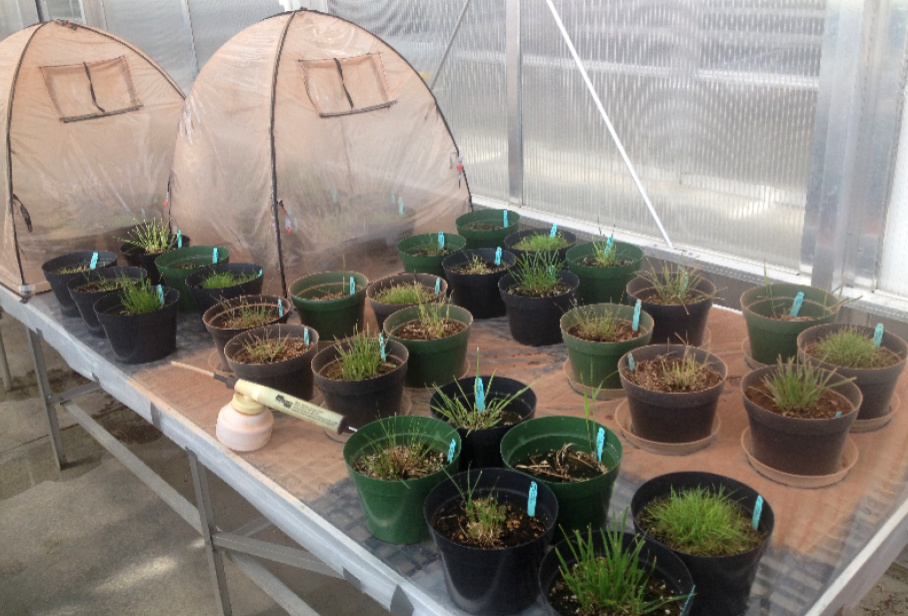
\includegraphics[width=2.2in, 
		trim={0cm 0cm 0cm 0cm}, clip=true]
		{science/GreenhouseDust}
		\caption{Controlled application of dust on plant leaves in a greenhouse. 
			\label{fig:dust} } 
		% \index{Fire triangles!Fire behaviour|textit}
		% (Fig.~\ref{fig:dust})
	\end{center}
\end{marginfigure}

But working out in the natural environment at the scales that land is managed is different. 
The environment is inherently variable\textemdash only the most highly-managed field or pasture has exactly the same time of plants in the same type of soil on the same slope and with the same amount of moisture. 
Wildlands and other areas managed for wildlife, native plants, and general biodiversity conservation are notoriously variable in terms of topography, soil, hydrology, and plant communities.

	\chapter{Fuels} 

Fuel for wildland fire consists of vegetation. 
Recall from Eq.~\ref{eq:combustion} that combustion is essentially the decomposition of plant matter\textemdash originally produced by photosynthesis\textemdash in the presence of oxygen and sufficient heat. 
Because a high degree of variability in fire behavior can be attributed to variability in fuels, making good fuel measurements is essential to predicting how a prescribed fire will burn and explaining variability in the effects that fire produces. 

\section{Broad considerations}

\subsection{Fuels and the fire regime}

The primary consideration of fire regime in planning fuels measurement is identifying the \emph{fire type} by determining which vegetation layer(s) carries the fire (Fig.~\ref{fig:ParametersFactors}). 
Under all but the most extreme conditions in densely-wooded vegetation, prescribed fire management is typically focused on surface fires that consume herbaceous vegetation rooted in\textemdash or laying on\textemdash the soil surface. 
\footnote{Note that in woodlands and savannas, the fuelbed often contains leaf litter that fell from tree canopies, which are considered surface fuels once they have fallen.}

Next, one must determine if live fuel is a consideration (we assume here that it is). 
How to determine if live fuels are relevant? 
Consider the conditions below. 
If any apply to a burn or study, one should likely be measuring live and dead fuels separately: 

\paragraph{Checklist for live fuel relevance} 
\begin{itemize}
	\item[{\color{BisonGreen!80}\ding{51}}] Prescription for growing season burn
	\item[{\color{BisonGreen!80}\ding{51}}] Vegetation dominated by exotic cool-season (C\textsubscript{3}) grasses
	\item[{\color{BisonGreen!80}\ding{51}}] Management and/or research objectives focus on any C\textsubscript{3} grass
	\item[{\color{BisonGreen!80}\ding{51}}] Research objectives include parameterizing custom fuel models and/or modeling fire behavior  
\end{itemize}

However, if none of the above conditions apply, one is probably not missing out on much information by not dividing the fuelbed up into live and dead components.

There are two basic types of information on fuels the fire scientist ought to obtain \emph{by fuel class}\footnote{While these would typically also be described by size class, in the workshop we are considering only 1 hr fuels, so we will consider each in terms of live and dead components.}: 

\begin{itemize}
	\item Fuel load 
	\item Fuel moisture
\end{itemize}

\subsection{Sampling approaches}

There are two broad categories of sampling methodologies, each with pros and cons specific to wildland fuel sampling, although the pros and cons likely apply to other sampling contexts, as well: 
\begin{itemize}
	\item \textbf{Destructive\textemdash}Samples are collected by physically removing material from the environment. 
	\begin{itemize}
		\item[\textit{Pros:}]Most accurate; probably needs fewest observations. Raw data in desired units (mass/area for fuel load, \% $H_{2}O$ for fuel moisture).
		\item[\textit{Cons:}]Removes from the fire environment the very thing one seeks to describe within the fire environment. 
		Time consuming. 
		Requires weighing and drying equipment.
		Data not instantaneously available. 
	\end{itemize}
	\item \textbf{Non-destructive\textemdash}Sampling consists of observations that do not require the material to be disturbed. 
		\begin{itemize}
		\item[\textit{Pros:}]Doesn't remove any fuel from the fire environment. Most often requires less sample processing time \& effort, and data can be instantaneously available. 
		\item[\textit{Cons:}]Likely requires more observations to minimize variability. Raw data rarely on a meaningful scale; often needs a conversion factor that in turn must often be derived from separate calibration efforts.
	\end{itemize}
\end{itemize}

Whether one implements destructive or non-destructive sampling has profound implications on the nature of the sampling protocol and the data it produces, including the transferability of data to other events and locations and even whether the data are useful for the stated purposes. 
Consider just a few examples of how different wildland fire professionals might need different types of data on different time scales: 
\begin{itemize}
	\item \emph{The burn boss wants to make tactical decisions on fuel conditions such as a minimum or maximum fuel load, or minimum dead fuel moisture.} 
	They will need this information the day of the burn\textemdash they cannot wait for samples to be clipped, dried for 48 h, and weighed. 
	On the other hand, an estimation based on a representative but limited sample is probably sufficient. 
	The values likely do not need to be applied to other locations. 
	\item \emph{The biologist has designed a monitoring program to assess shrub mortality across several sites with different amounts of smooth brome.} 
	Whether that smooth brome was green or not at the time of the fire\textemdash and how much of it there was\textemdash is likely important information. 
	On the other hand, categorical assessments of live:dead biomass based on non-destructive observations is probably sufficient.
	An estimation of live fuel moisture based on a representative but limited sample would probably be icing on the cake. 
	\item \emph{A graduate student has a hypothesis that connects fire behavior to fuel parameters.} 
	It is important that multiple pre-fire measurements be taken around each fire behavior observation point, and continuous variables are best. 
	On one hand, statistical analysis can take fuel load on any scale, so a rapid, non-destructive quantification method will be fine.
	On the other hand, reviewers are likely going to want to be able to connect these data to actual values, and managers will need those values to apply the findings well, so it is best to have a plan for calibration. 
	An accurate measure of fuel moisture is important, but the data aren't needed until well after the fire, so there is plenty of time to dry and weigh clipped samples. 
\end{itemize}  

These questions help guide a responsive and informative sampling plan: 

\begin{itemize}[noitemsep]
	\item[] \hspace{-1.9em}\emph{Ask first:}
	\item[{\color{BisonGreen!80}\ding{51}}]\emph{Who} is expecting the data and \emph{what} are they going to use it for?
	\item[{\color{BisonGreen!80}\ding{51}}]\emph{When} are they expecting it?
	\item[] \hspace{-1.9em} \emph{Then determine:}
	\item[{\color{BisonGreen!80}\ding{51}}]\emph{What} will be reported
	\item[{\color{BisonGreen!80}\ding{51}}]\emph{How and when} data will be collected 
\end{itemize}

\section{Measuring fuel load} 

\subsection{Destructive sampling}

Clipping is the most straightforward form of measuring fuel load in grasslands. 
A representative sample point is identified, a known area determined, and all vegetation\textemdash representing combustible fuel\textemdash is removed by hand and stuffed into a paper bag (Fig.~\ref{fig:clipping}). 
Once dried and weighed, the mass of the material in the bag is easily expressed as the fuel load for the known area from which the sample was collected.

\begin{figure*} 
		\begin{center}
	\includegraphics[width=0.57\textwidth]
		{science/Fuels/ClippingQuadratShears}~
	\includegraphics[width=0.43\textwidth]
		{science/Fuels/DryGrassBag}
			\end{center}
	\caption{On the left, a 0.25 mm\textsuperscript{-2} quadrat is about to be clipped with sheep shears (this might sound silly, but they are the secret weapon for efficient grass clipping). 
		Once bagged, the samples are dried in a forced air drying oven at at least 60$\deg$C for at least 48 h. 
		After drying, samples are weighed and their mass expressed on a per-area basis.
		 } \label{fig:clipping}
	%(Fig.~\ref{fig:clipping})
\end{figure*}

\paragraph{Clipping} 

Clip all material to within about 2 cm or 1 inch of the soil surface. 
The main idea is to gather as much combustible material as possible while being as consistent from sample to sample. 
Clipping and scraping right down to bare mineral soil when one can will produce a different picture of the available fuel load than a quadrat with a thicker mat of wet litter that is unlikely to burn anyway (Fig.~\ref{fig:residue}). 
Better to be consistent from quadrat to quadrat. 
Deposit clipped material in a paper bag clearly labeled with a marker. 

\begin{marginfigure}
	\begin{center}
		\includegraphics[width=2.2in]
		{science/fuels/residue}
		\caption{Even a hot fire can't burn it all off. 
			\label{fig:residue} } 
		% (Fig.~\ref{fig:residue})
	\end{center}
\end{marginfigure}

\paragraph{Drying}

Clipped biomass samples are typically dried in forced-air ovens at at least 60$\deg$C.\footnote{There is debate around the minimum temperature required to adequately dehydrate samples, although differences have the most effect on determining moisture content, not dry mass. 
	Thus this debate is discussed in the fuel moisture section below.}
The aim is to dehydrate clipped biomass to the point that the samples reach an equilibrium moisture content with the air in the oven\textemdash as the weight of samples at such a state would no longer loose mass, complete drying of samples is often referred to as ``constant mass.``
With herbaceous samples, this often occurs within 48 hours. 
 
\paragraph{Weighing}

Weigh dried biomass samples on a digital balance shortly after removal from the oven, before they absorb moisture from the cooler ambient air. 
The primary concern with weighing is accounting for the mass of the paper bag. 
One can either dump the bag contents into a tared container on the balance, or weigh the sample in the bag and subtract the mass of the bag. 
There are many arguments for the latter\textemdash it is often faster and less messy\textemdash but it is prone to error if different types of bags are used. 
A best practice for data management is to enter a code for the bag type when entering mass data for each sample, or group of samples with a common bag type, and assign the mean mass of several empty bags to each code when subtracting bag weights prior to analysis. 
	


\subsection{History of fire in grasslands}

Fire has been an intrinsic component of grasslands and other rangeland ecosystems since these biomes developed and spread around the world. 
Grasslands as we know them today\textemdash including both the vegetation and characteristic animal communities\textemdash emerged after the last Ice Age, and have burned regularly and naturally since. 
Many grass-dominated landscapes owe their existence to fire, especially in the US Great Plains \citep{mcgranahan2021}, where precipitation is substantial enough to support woody plant species capable of converting these landscapes to shrublands, woodlands, or even forests without regular burning. 



\begin{marginfigure}
	\begin{center}
		
\includegraphics[width=2.2in, 
				trim={1.5cm 0cm 1cm 0.5cm}, clip=true]
			{groundhogday}
		\caption{Topography, weather, and the fuelbed are the three major drivers of wildland fire behaviour.
			\index{Fire triangles!Fire behaviour|textit} \label{fig:FireBehaviourTriangle} } 
		% (Fig.~\ref{fig:FireBehaviourTriangle})
	\end{center}
\end{marginfigure}
	\chapter{Fire weather}
\label{ch:weather}

Weather is the most variable component of the fire behavior triangle (Fig.~\ref{fig:FireBehaviorTriangle}). 
Understanding effects of weather on fire behavior is key to safely conducting any fire management\textemdash wildland fire use or suppression\textemdash and provides important information to understanding variability in fire behavior even if fuels are relatively similar. 

 \begin{marginfigure}
	\begin{center}
		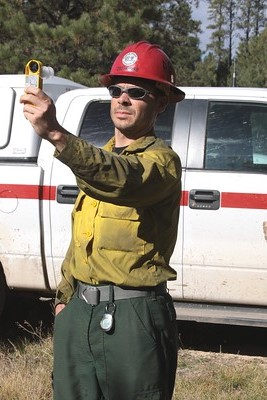
\includegraphics[width=2.2in, 
		trim={0cm 3cm 1cm 1cm}, clip=true]
		{science/weather/UsingKestrel}
		\caption{Devices like portable weather meters make it easy to quickly collect fire weather information to support tactical decisionmaking and ecological research.  
		\label{fig:UsingKestrel} } 
		% (Fig.~\ref{fig:UsingKestrel})
	\end{center}
\end{marginfigure}

Wildland fire weather information can be divided into two components \citep{teie2018}: 

 \begin{itemize}[noitemsep]
	\item \textbf{Strategic weather\textemdash}Information on general trends for a day, extending to several days. 
	\item \textbf{Tactical weather\textemdash}Local observations made at the scene (Fig.~\ref{fig:UsingKestrel}).
Typically includes air temperature (often called \emph{dry bulb}), relative humidity, and a wind vector (direction, average sustained wind speed, peak gust).
\end{itemize}

Below we describe how to acquire and use both types of data in a prescribed fire operation.
From an operational perspective, strategic weather information consists of forecasts and tactical weather information comes from belt weather kits and local automated weather stations. 
Researchers have access to the same forecast data but also historical data at multiple scales, from automatic weather stations that log data and are networked, to broad-scale, gridded historical weather data products. 

\section{Strategic weather}

Strategic weather products consist primarily of forecasts available from a number of sources at several different spatial and temporal scales.\footnote{We focus here on shorter-term products from the National Oceanic and Atmospheric Administration's National Weather Service (\href{https://www.weather.gov}{weather.gov}), but NOAA's \href{https://www.spc.noaa.gov/products/fire\_wx/overview.html}{Storm Prediction Center} and \href{https://www.cpc.ncep.noaa.gov/products/Drought/}{Climate Prediction Center} also offer longer-term outlooks relevant to fire planning.
	Additionally, the National Interagency Fire Center's Predictive Services provide a lot of fire-specific weather information at both national and regional levels (\href{https://www.predictiveservices.nifc.gov/weather/weather.htm}{predictiveservices.nifc.gov/weather/weather.htm}). 
	The information is geared towards wildland fire suppression but is also useful for prescribed fire operations. }

\subsection{Forecast products} 

The National Weather Service (NWS) provides several products either specifically for, or very relevant to, fire weather. 
We discuss a few here, starting at spatially-broad and long time scales, working to local predictions for specific time periods at a specific point on the landscape. 

\subsubsection{Basic weather products}
NWS provides extended outlooks at a national scale (Fig.~\ref{fig:ExtendedOutlookExample}). 
Each NWS office also provides a daily Area Forecast Discussion that not only explains how current regional atmospheric patterns affect the area's weather, but also some of the considerations taken into account by local forecasters as they assess model output.

\begin{figure} 
	\begin{center}
		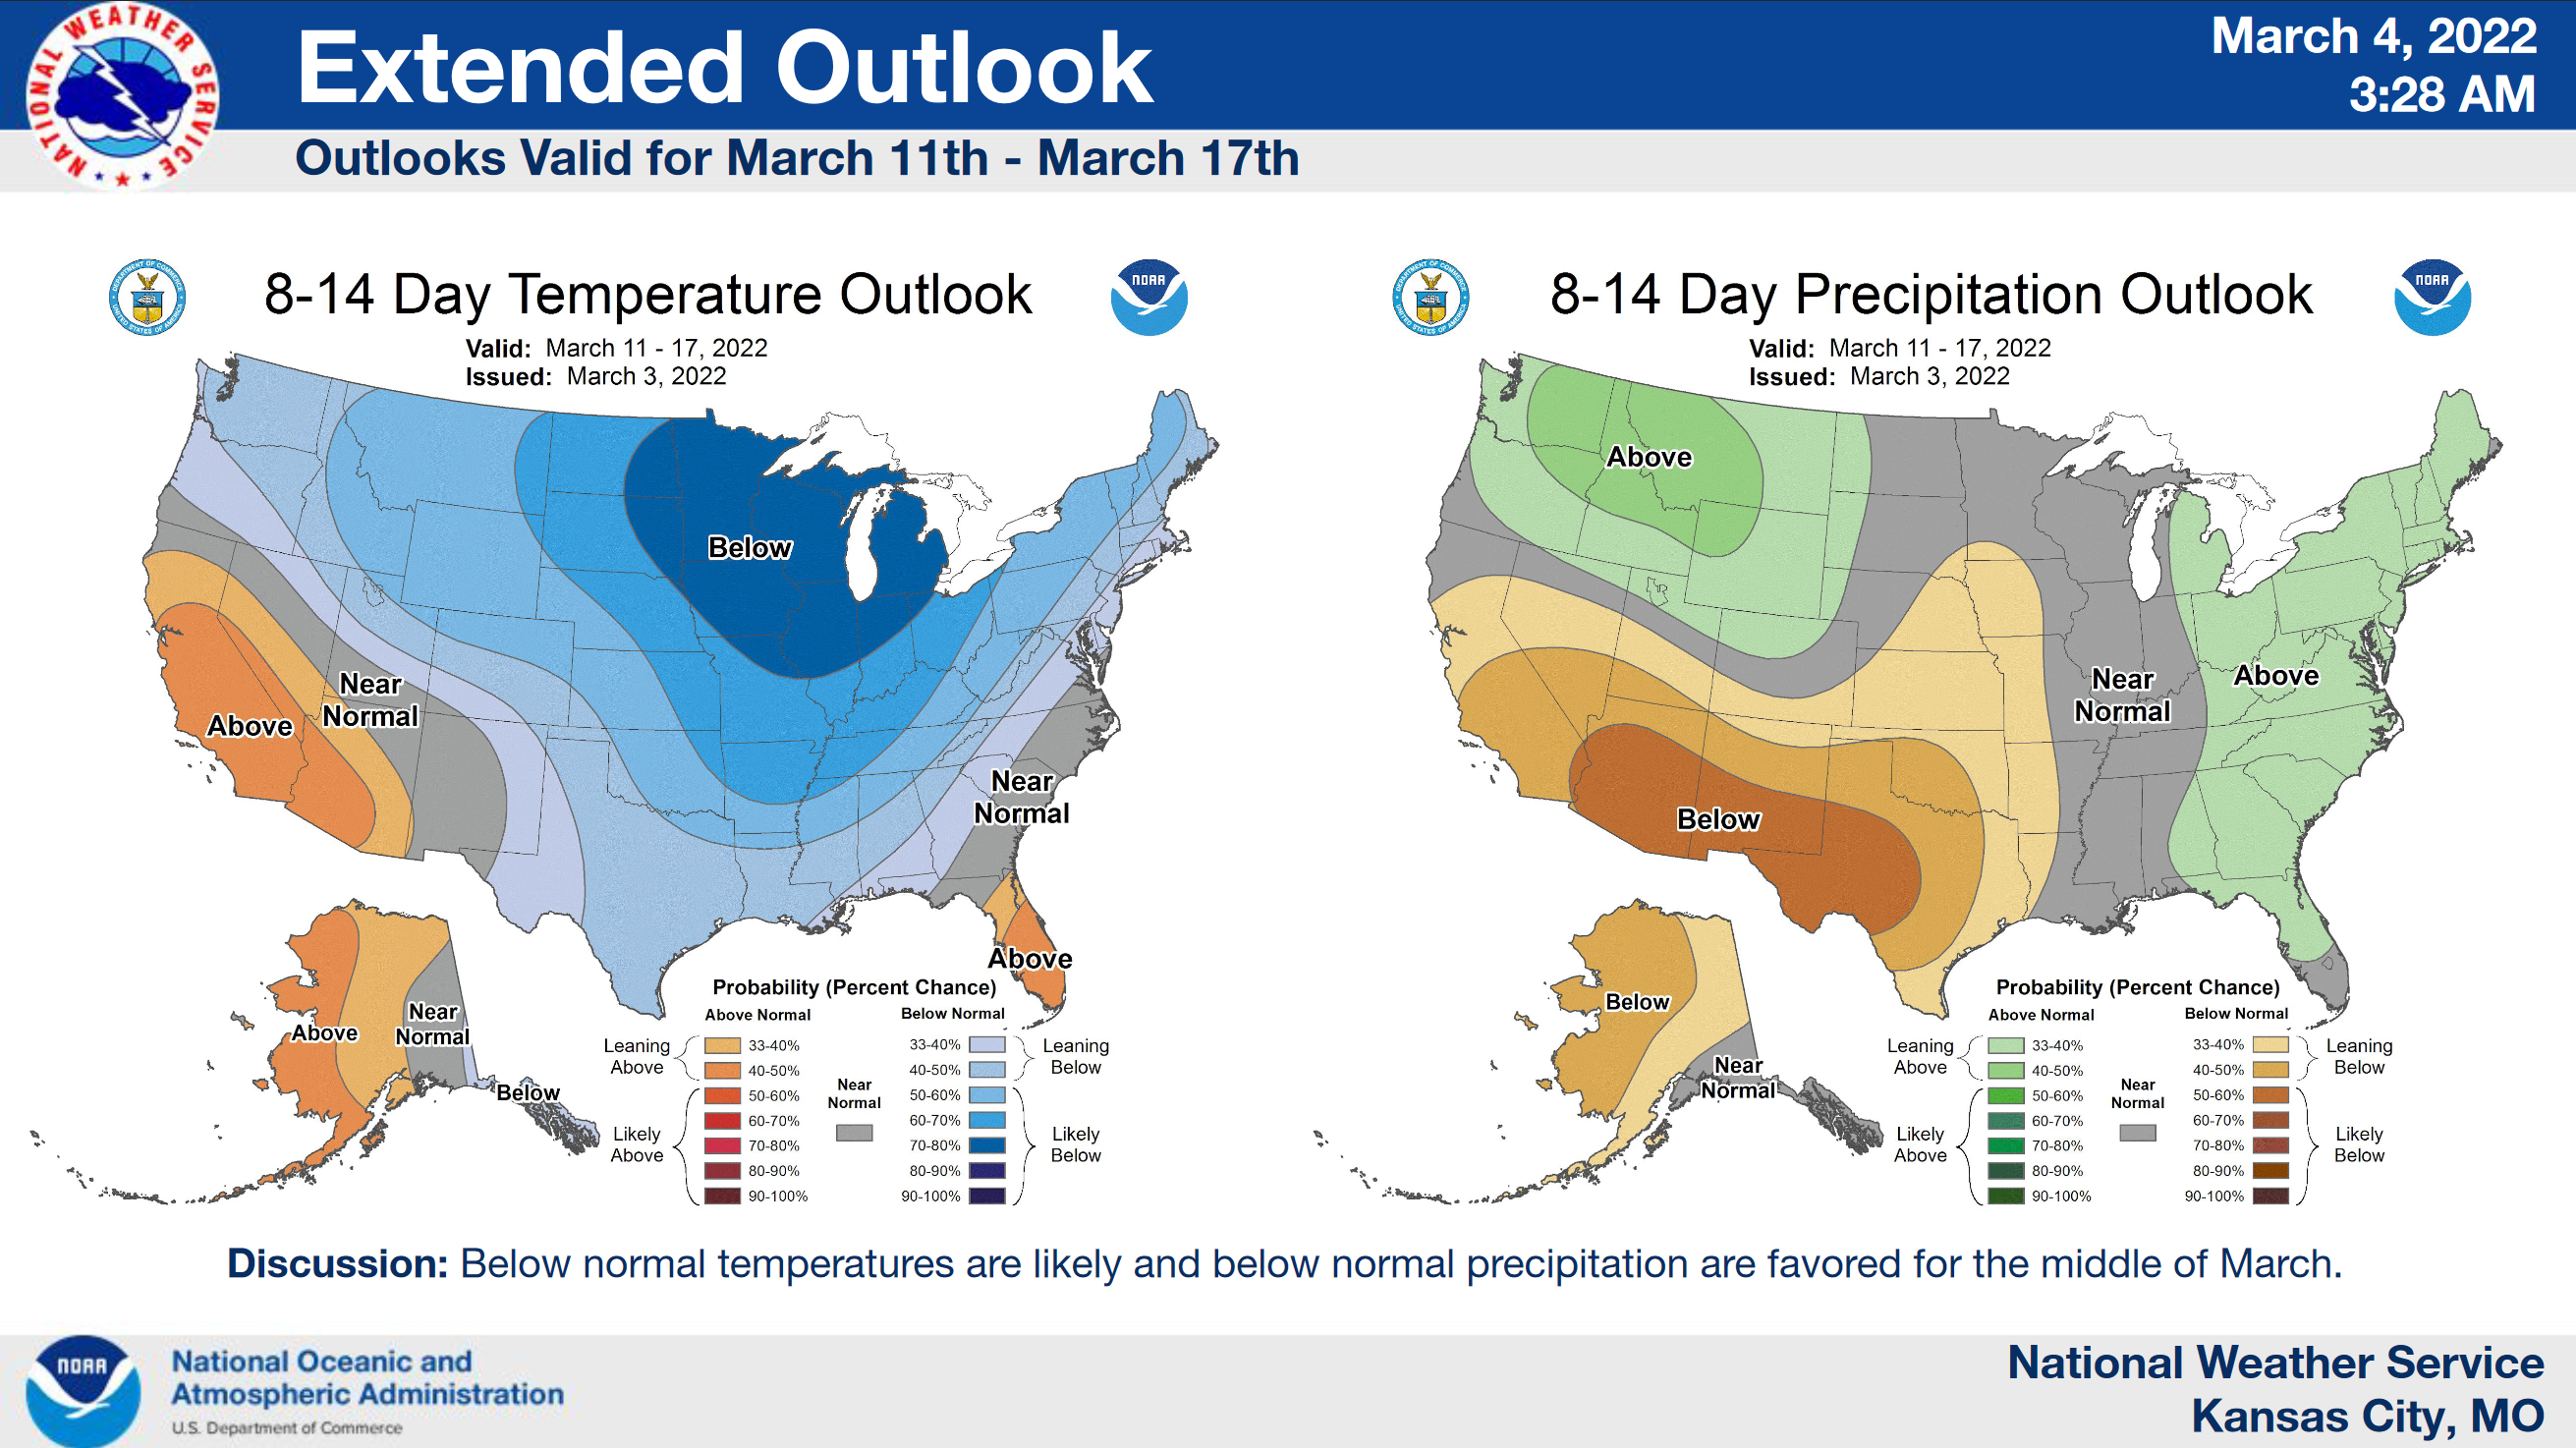
\includegraphics[width=1\textwidth]
		{science/weather/ExampleNationalExtendedOutlook}
		\ImageCredit{https://www.weather.gov/media/eax/DssPacket.pdf, 4 March 2022}
	\end{center}
	\caption{An example of national 8-14 day temperature and precipitation outlooks provided by the Kansas City, MO NWS office.
	} \label{fig:ExtendedOutlookExample}  
	%(Fig.~\ref{fig:ExtendedOutlookExample})
\end{figure} 

Zone area forecasts\textemdash accessible by searching a town name at \href{http://weather.gov}{weather.gov}{}\textemdash are local forecasts generated at the county or municipality level by regional NWS offices.
Zone area forecasts provide a 7-day weather forecast and current conditions at the nearest NWS observation point, typically the closest airport. 
These pages also provide hourly weather forecasts that illustrate predicted trends in several weather variables hour-by-hour over the next few days (Fig.~\ref{fig:BasicHourlyExample}).

\begin{figure} 
	\begin{center}
		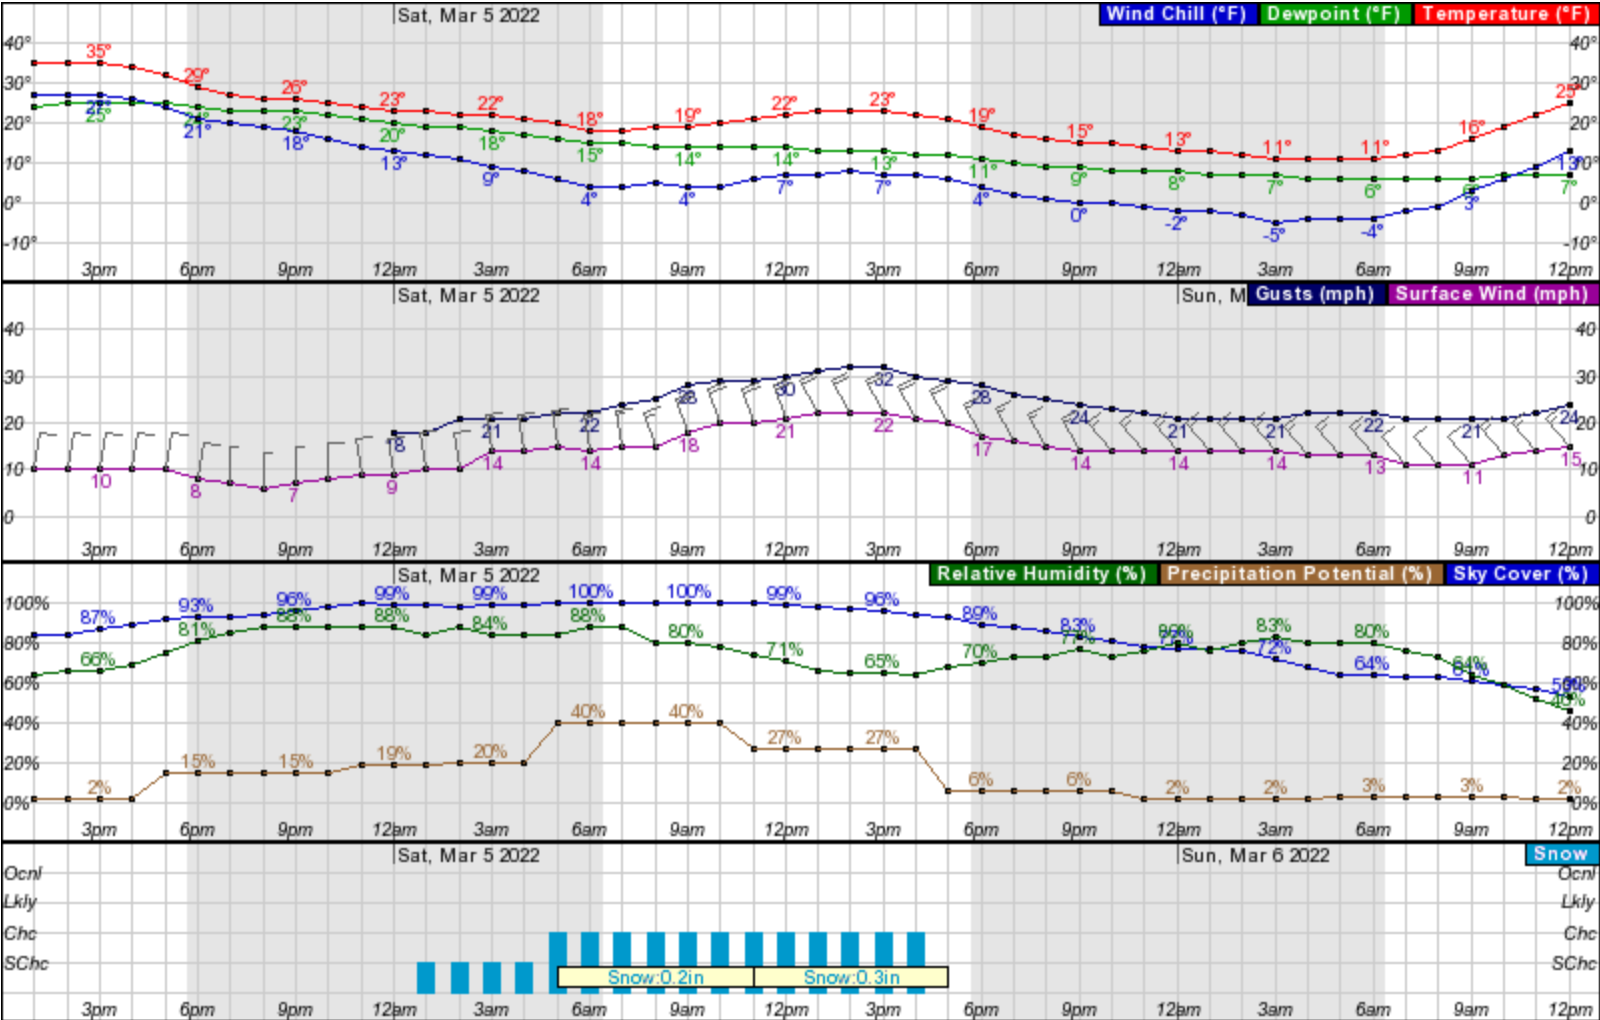
\includegraphics[width=1\textwidth]
		{science/weather/BasicHourlyExample}
	\end{center}
	\caption{An example of predicted hourly trends in several basic weather variables for two days in Hettinger, North Dakota. 
		All regional NWS offices in the country provide this product.
		While searched best by town names (\href{http://www.weather.gov}{weather.gov}), one can edit the latitude and longitude fields in the URL by hand to generate an hourly forecast for a specific point and bookmark it for future use. 
	} \label{fig:BasicHourlyExample}
	%(Fig.~\ref{fig:BasicHourlyExample})
\end{figure}  

\subsubsection{Specific fire weather products} 

\begin{figure}
	\caption{Two examples of national fire-related forecast products conveniently posted at \href{https://www.weather.gov/fire/}{weather.gov/fire}, but produced elsewhere: the wildfire potential outlook product is generated by the \href{https://www.predictiveservices.nifc.gov}{National Interagency Fire Center's Predictive Services} while the drought monitor comes from the \href{https://droughtmonitor.unl.edu/}{University of Nebraska\textendash Lincoln}. 
	} 
	\begin{center}
		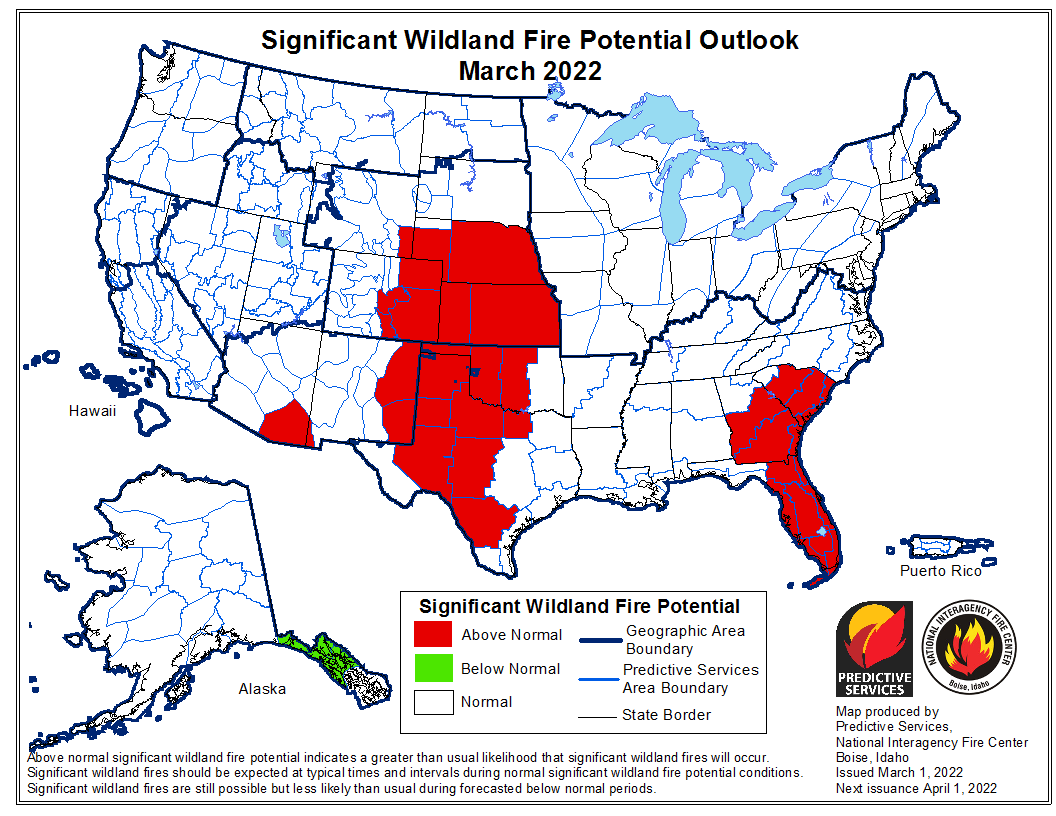
\includegraphics[width=0.5\textwidth]
		{science/weather/MonthOutlookExample}~
		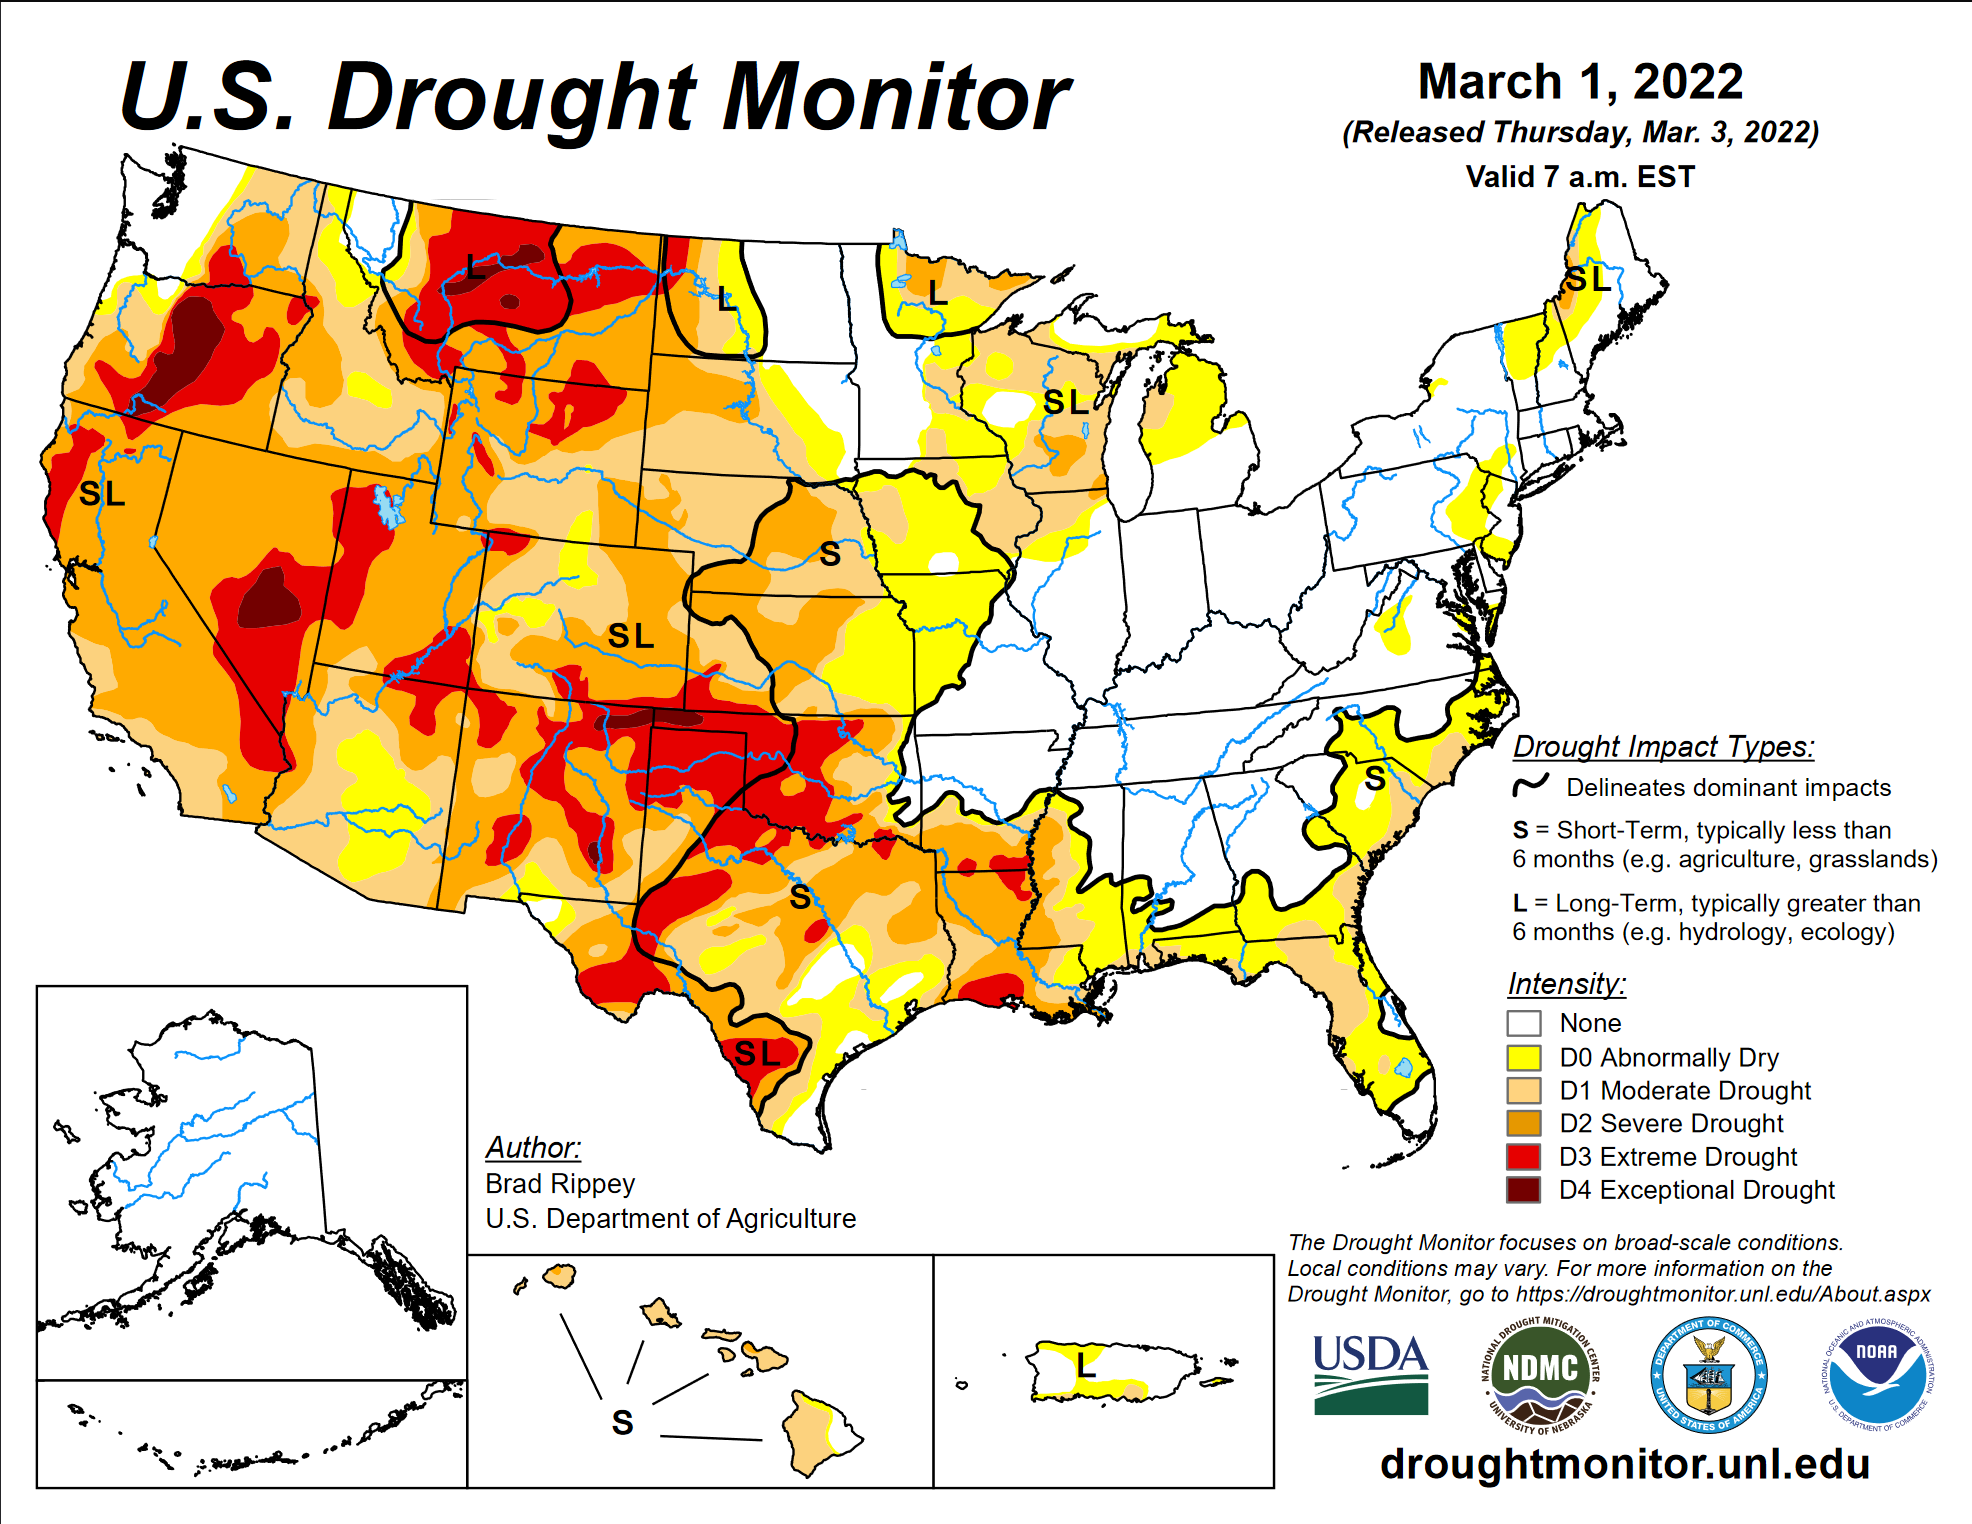
\includegraphics[width=0.5\textwidth]
		{science/weather/DroughtMonitorExample}
	\end{center}
	\label{fig:NationalProducts}
	%(Fig.~\ref{NationalProducts})
\end{figure}

National fire-related forecast data are compiled at \href{https://www.weather.gov/fire/}{weather.gov/fire (Fig.~\ref{fig:NationalProducts})}. 
Some regional NWS offices provide fire-specific forecast information. 
\href{https://forecast.weather.gov/product\_sites.php?site=NWS\&product=FWF}{Several regional offices around the country} provide text-based Routine Fire Weather Forecasts that give strategic fire weather forecasts for smaller zones within the area (Fig.~\ref{fig:RoutineFireFcstExample}).
But not all offices provide fire-specific data, and not all regions provide the same information or even for the whole year.
For example, Bismarck, ND regional office has \href{https://www.weather.gov/bis/fire\_managers}{a page dedicated to fire weather in western and central North Dakota}, but it isn't maintained during winter months.
And compare differences in output between Figs.~\ref{fig:RoutineFireFcstExample} \& \ref{fig:SpotExample} due to different local environmental contexts.  

\begin{figure} 
	\begin{center}
		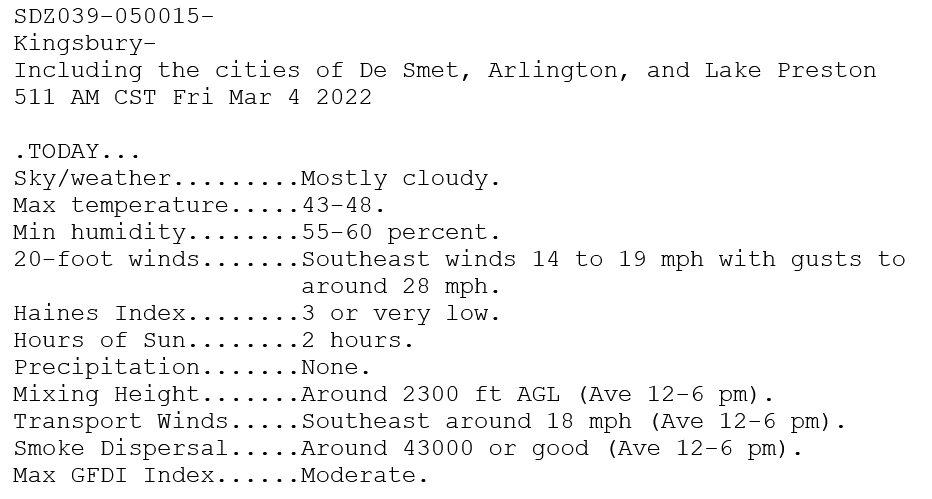
\includegraphics[width=1\textwidth]
		{science/weather/RoutineFireFcstExample}
	\end{center}
	\caption{An example of a Routine Fire Weather Forecast for Kingsbury County, South Dakota. 
		Note that because much of South Dakota wildland fire occurs in rangeland, many NWS offices in the state calculate a Grassland Fire Danger Index (GFDI). 
	} \label{fig:RoutineFireFcstExample}
	%(Fig.~\ref{fig:RoutineFireFcstExample})
\end{figure}  

\paragraph{Spot weather forecasts}
	
A spot weather forecast is a ''special forecast issued to fit the time, topography, and weather of a specific incident.''\footnote{\citet[Spot Weather Forecast][]{nwcg2019}}
The forecast includes information similar to the routine fire weather forecast  (Fig.~\ref{fig:RoutineFireFcstExample}), but a specific NWS forecaster concentrates predictive weather models on a specific location provided by a request filed by a qualified user at \href{https://www.weather.gov/spot/}{weather.gov/spot}. 
Requests include the geospatial location and date along with some site-specific information, such elevation above sea level, fuel type, slope and aspect, and size of burn. 
The results include a description of general weather patterns expected for the day, as well as specific predicted values for fire-related variables at critical points in the day (Fig.~\ref{fig:SpotExample}).

\begin{figure} 
	\begin{center}
		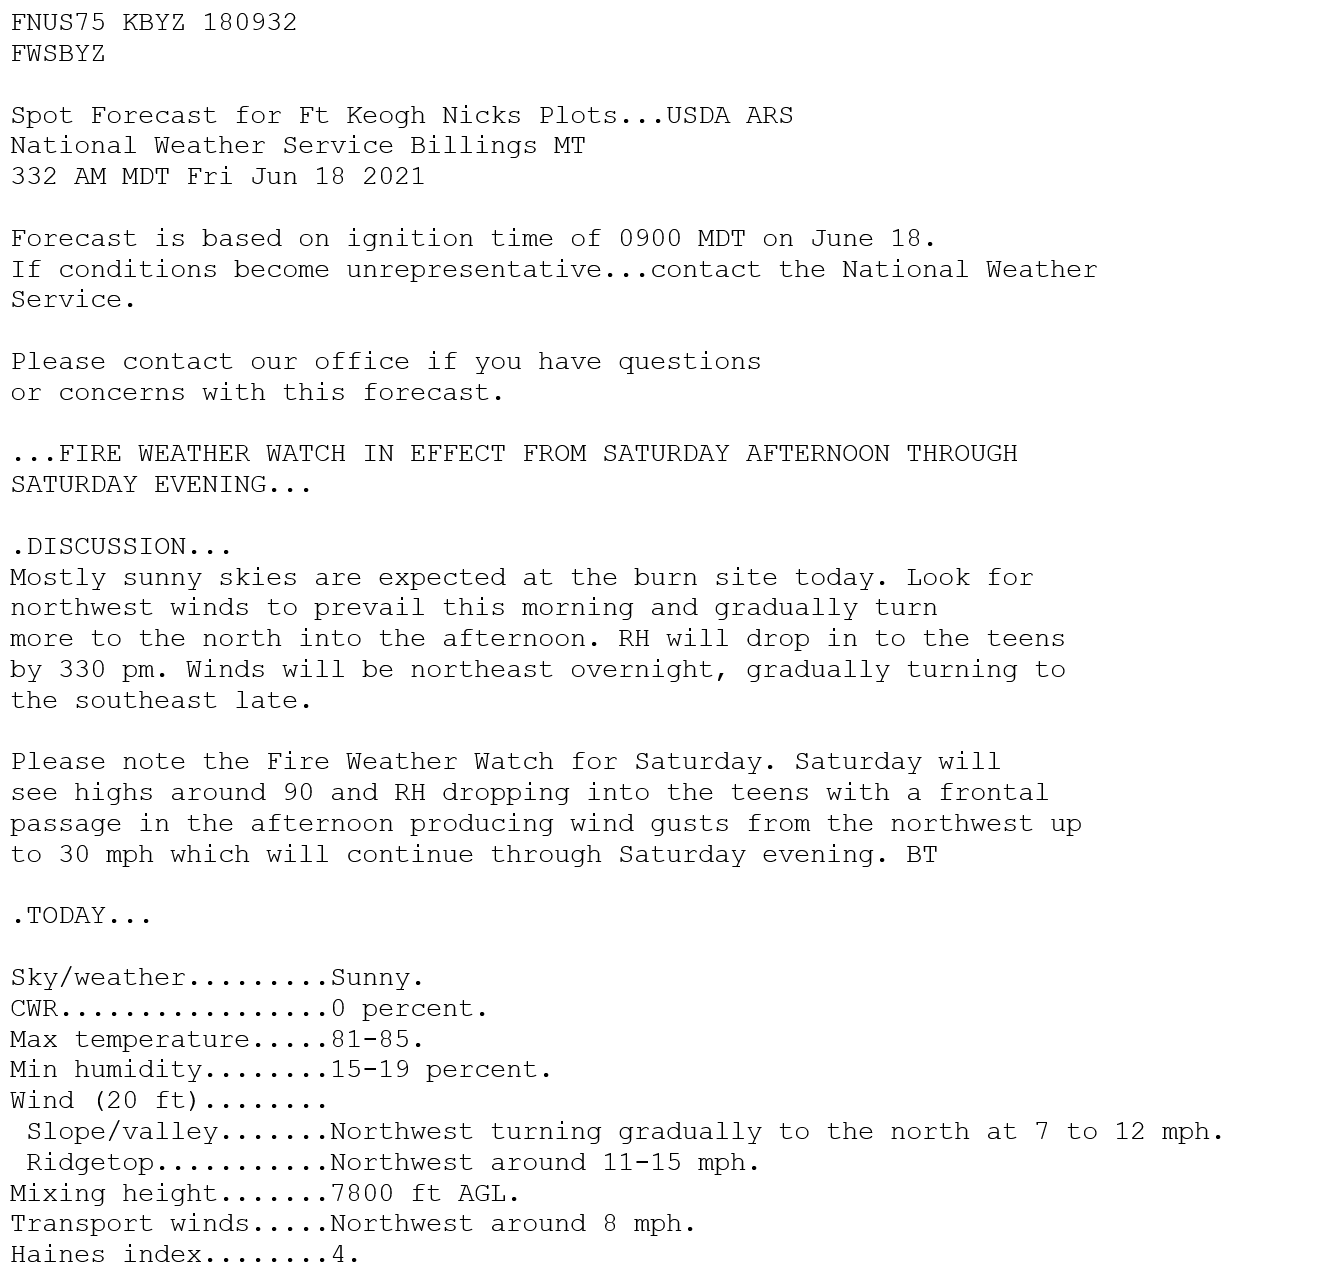
\includegraphics[width=1\textwidth]
		{science/weather/SpotExample}
	\end{center}
	\caption{An example of a Spot Weather Forecast for a summer prescribed burn generated by the NWS regional office in Billings, MT.
		Note that because the Billings office covers mountainous areas, forecasters account for topographical effects on wind by breaking wind predictions  down for slope/valley and ridgetop positions. 
		Note also that the forecast was generated at 03:33, and the forecaster calls attention to a fire weather watch in effect for the next day, with a description of the anticipated weather changes. 
		As the ignition time approached and observed winds were higher than predicted, the NWS staff member who generated the spot forecast contacted the burn boss via the cell phone number provided in the request. 
		After a discussion with local fire management officials about existing fire danger conditions and the expected trend towards extreme weather, this prescribed fire operation was postponed. 
		It is impossible to determine whether this burn would have been a success or a failure had the burn boss proceeded. 
		But by working with the NWS and county officials, the burn boss was certainly aware of the current and forecast conditions when considering the Go/No-go decision. 
	} \label{fig:SpotExample}
	%(Fig.~\ref{fig:SpotExample})
\end{figure} 

The official NWS spot forecast process is not the only way to obtain location-specific information. 
Regional offices that provide fire services also provide fire-specific products in the hourly weather forecast format (Fig.~\ref{fig:FireHourlyExample}). 
Even managers who obtain official spot weather forecasts can complement that information, which focuses on weather at critical times of the day, with hourly predictions of the same fire-specific variables. 

\begin{figure} 
	\begin{center}
		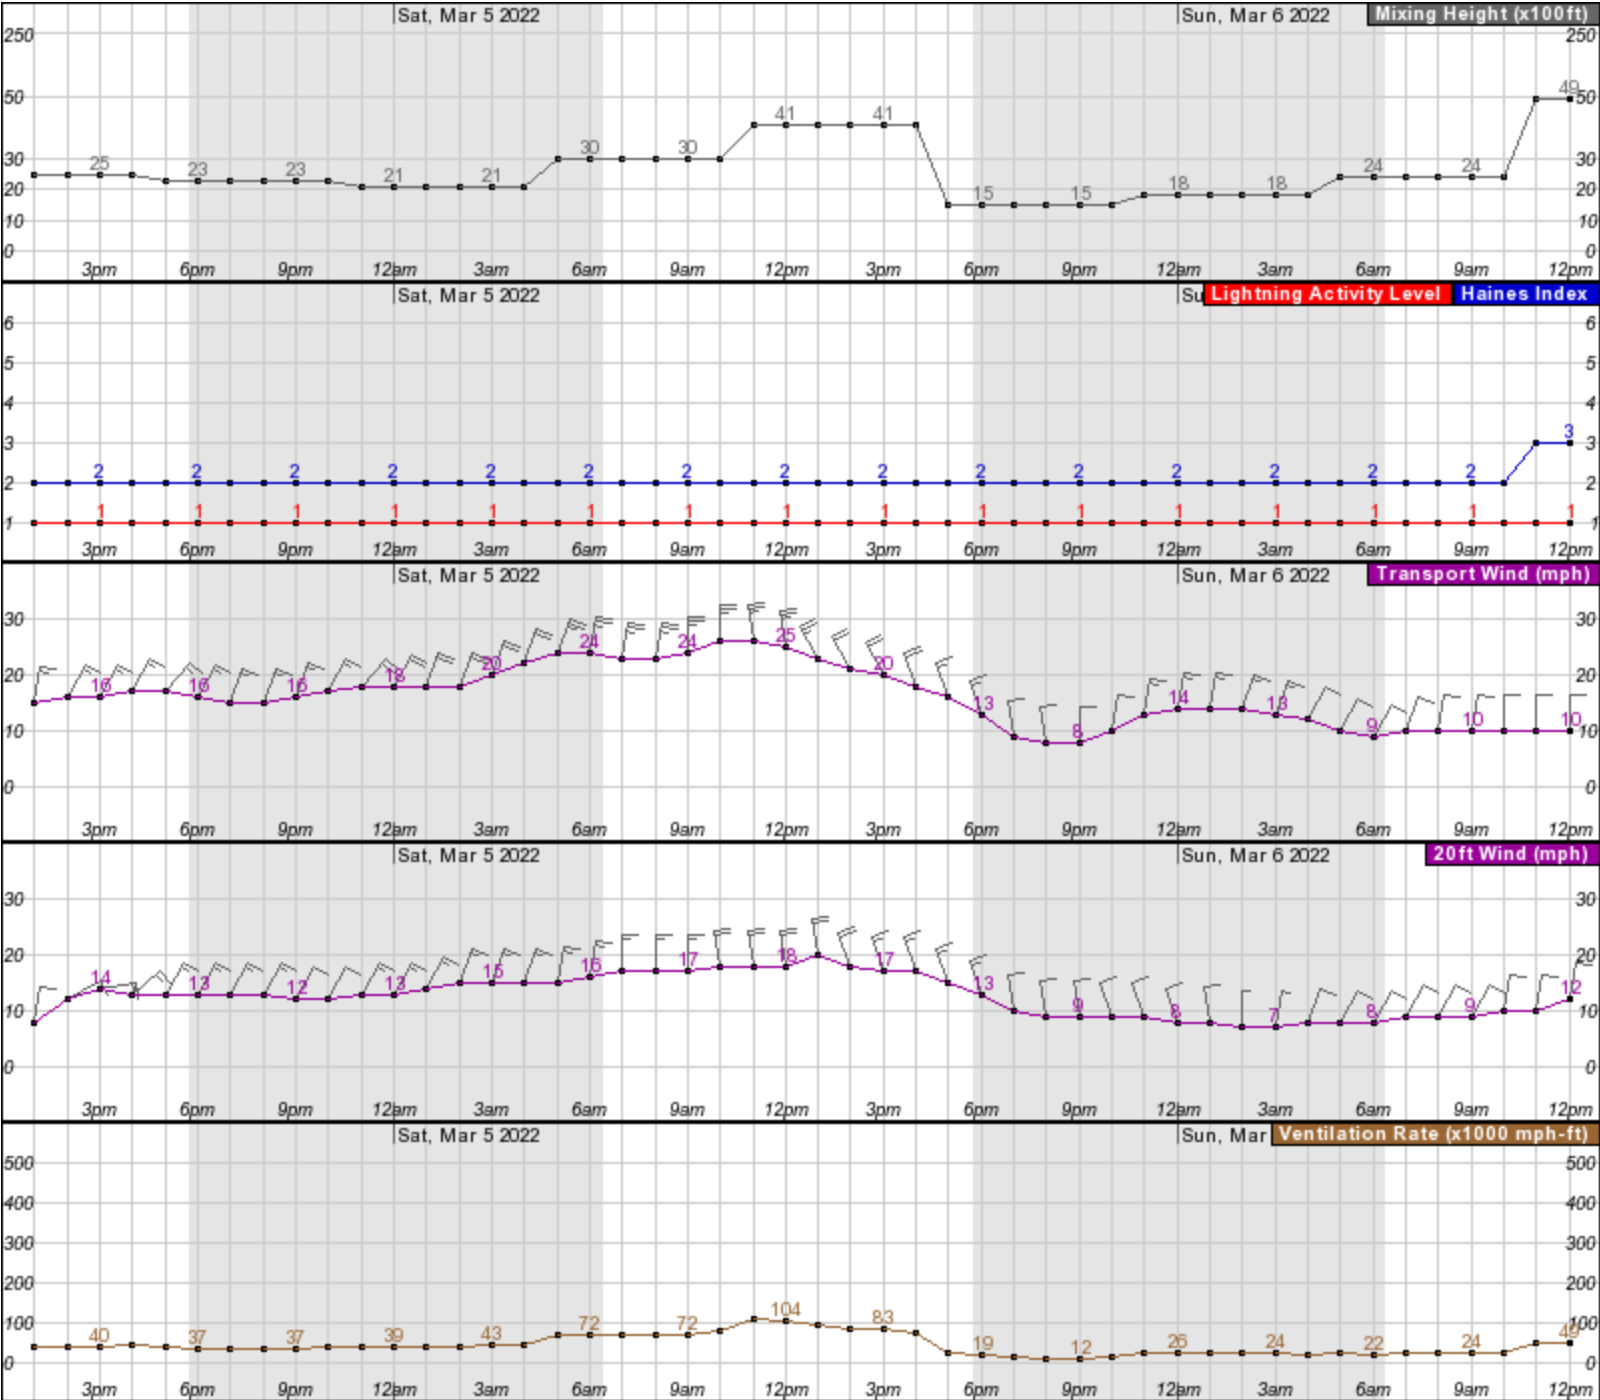
\includegraphics[width=1\textwidth]
		{science/weather/FireHourlyExample}
	\end{center}
	\caption{An example of predicted hourly trends in several variables specific to wildland fire for two days in Chadron, Nebraska. 
		Not all regional NWS offices in the country provide fire products, and the specific fire products provided varies among offices. 
		The hourly weather format can be ``hacked'' to provide location-specific information by hand-editing the longitude and latitude fields of the URL for an hourly weather product found for a local town.
	} \label{fig:FireHourlyExample}
	%(Fig.~\ref{fig:FireHourlyExample})
\end{figure}  

\section{Tactical weather}

Fire managers and researchers alike rely on real-time fire weather observations taken during the operational period.

\begin{figure} 
	\begin{center}
		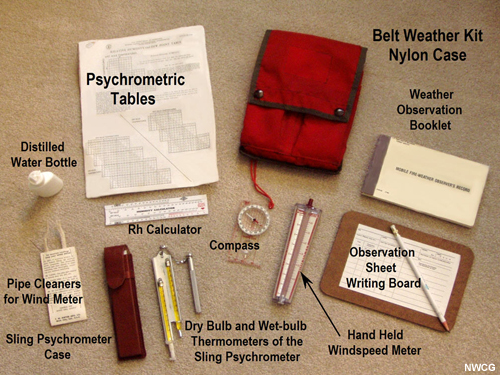
\includegraphics[width=1\textwidth]
		{science/weather/BeltWeatherKit}
	%	\ImageCredit{NWCG}
	\end{center}
	\caption{Standard items in the belt weather kit for making fire weather observations in the field. 
	} \label{fig:BeltWeatherKit}
	%(Fig.~\ref{fig:BeltWeatherKit})
\end{figure} 

\subsection{Spinning weather}

The tried-and-true methods of taking fire weather measurements are included in the \emph{belt weather kit}, a standard package of field-ready instruments for measuring and recording air temperature, dew point \& relative humidity, and wind speed \& direction (Fig.~\ref{fig:BeltWeatherKit}). 
Using the belt weather kit is sometimes called \emph{spinning weather} in reference to the sling psychrometer that is used for measuring dew point and relative humidity. 

While the belt weather kit has been technologically superceded by portable handheld weather meters (Fig.~\ref{fig:UsingKestrel}), it remains important to understand the operation of the belt weather kit because both methods have their own sources of error and opportunities for malfunction or damage. 
And one never knows when the batteries on the electronic meter will fail.
Finally, there is debate on which method is ``best.'' 
When both options are available, fire weather observers are advised to use both the belt weather kit and an electronic meter at least at the beginning of the observation period and make a note of which method was used to collect each value.  

Common tactical weather variables include: 

\begin{itemize}%[noitemsep]
	\item \textbf{Air temperature\textemdash}Often called \emph{dry bulb temperature} because ambient air temperature can be read from the unaltered thermometer on the sling psychrometer. 
	Air temperature is not a direct factor in fire behavior, but it helps managers understand trends in fuel moisture and crew well-being. 
	\item \textbf{Relative humidity (RH)\textemdash}As a measure of the capacity for the air to absorb moisture, RH is a critical variable in how quickly fuel dehydrates, and thus fire intensity. 
	Exposure to low RH desiccates fuels ahead of flame fronts and makes crew members more susceptible to dehydration. 
	RH is calculated by comparing measurements from a sling psychrometer via a psychrometic table or slide rule (Fig.~\ref{fig:SpinningWeather}, \emph{top}). 
	\item \textbf{Wind\textemdash}Wind is often reported as a \emph{vector} consisting of velocity and speed. 
	As ventilation increases oxygen available to the combustion reaction zone, wind increases fire intensity and drives rate of spread.  
	Wind speed is often reported as \emph{sustained}\textemdash an average value or range of wind speed over a minute or two\textemdash and \emph{gusts}\textemdash peak velocities that are substantially above the average or beyond the range of sustained winds. 
	Handheld anemometers measure wind speed (Fig.~\ref{fig:SpinningWeather}, \emph{bottom}). 
	A compass aids in determining wind direction. 
\end{itemize}

\begin{figure} 
	\begin{center}
		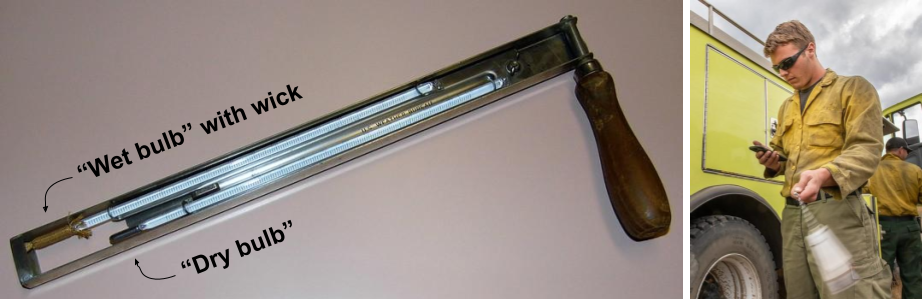
\includegraphics[width=1\textwidth]
		{science/weather/SlingPsychrometer}\\
		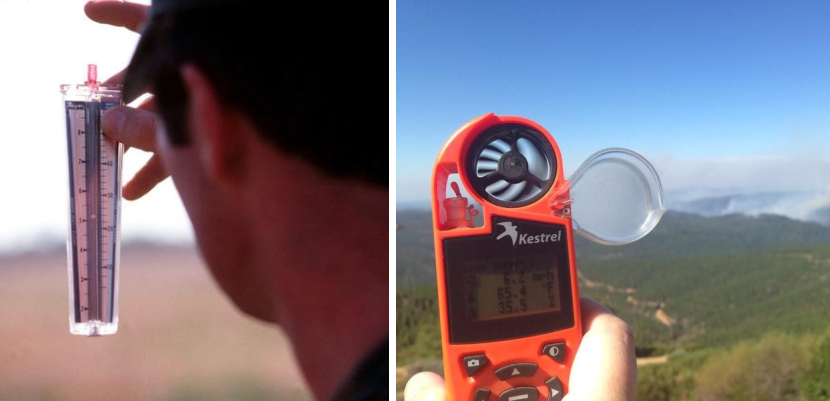
\includegraphics[width=1\textwidth]
		{science/weather/anemometers}
		\ImageCredit{TL: Joe Haupt, CC BY-SA 2.0; TR: Neal Herbert, US DOI, public domain; BL: USAF, public domain; BR: USDA, CC BY 2.0}
		\ImageIndex{CC BY-SA 2.0}
		{fig:SlingPsychrometer}
		{Joe Haupt}
		{https://www.flickr.com/photos/51764518@N02/19543105108}
	\end{center}
	\caption{Methods of taking fire weather observations. 
		\textbf{Top:} Sling psychrometers allow one to calculate instantaneous relative humidity by determining how quickly evaporation produces a cooling effect. 
		Left: An antique sling psychrometer with a wooden handle for spinning two thermometers, one open to the ambient air (``dry bulb'') and one with a ``wet bulb'' wrapped in a soaked wick that cools while the water evaporates while the device is spun rapidly. 
		A table or slide rule in the belt weather kit converts the difference between the final temperatures into dew point (DP) and relative humidity (RH). 
		Right: Belt weather kits include a small sling psychrometer with a chain connecting the thermometers to a chain, and smartphone apps quickly calculate DP and RH. 
		\textbf{Bottom:} Two methods for determining wind speed. 
		Left: Analog wind meter, standard in the belt weather kit. 
		Right: A Kestrel brand all-in-one portable weather kit. 
		Such units take digital measurements of many parameters of use to wildland fire professionals. 
	} \label{fig:SpinningWeather}
	%(Fig.~\ref{fig:SpinningWeather})
\end{figure}

 \begin{marginfigure}
	\begin{center}
		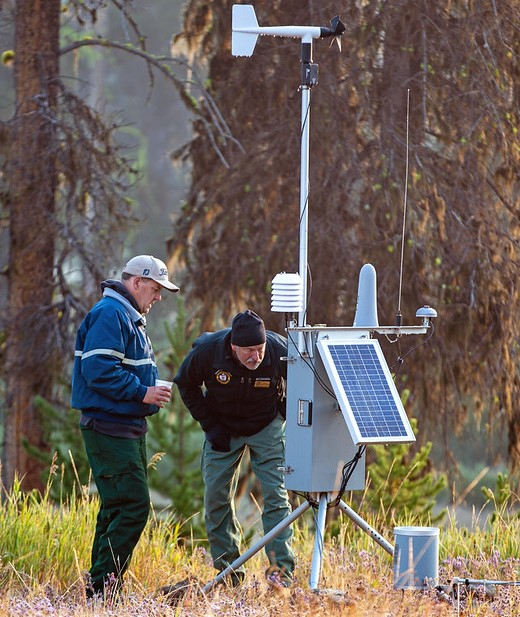
\includegraphics[width=2.2in]
		{science/weather/CheckingRAWS}
		\caption{Technicians service a Remote Access Weather Station (RAWS) that provides real-time fire weather (and sometimes fuel moisture) data to fire managers. 
			Unlike NWS observations, which are typically made at airports, RAWS stations are typically placed in representative wildland fuelbeds.
			 \label{fig:RAWS} } 
		% (Fig.~\ref{fig:RAWS})
	\end{center}
\end{marginfigure}

\subsection{Automated weather stations}

Additionally, hourly weather observations made by the NWS and even Remote Access Weather Stations managed by state and federal agencies are all available together online at MesoWest \href{https://mesowest.utah.edu/}{mesowest.utah.edu} (Fig.~\ref{fig:RAWS}).
Several states in the Midwest, especially, support \emph{mesonets}\textemdash networks of remote weather stations useful for agricultural purposes that provide both real-time and historical weather data useful for prescribed burners.  


\section{Historical weather data}



\paragraph{Point-level data} 

Many of the same resources for getting real-time observations from remote weather stations provide a means to access historical records. 
Substantial requests for historical MesoWest data can be managed via their API \href{https://developers.synopticdata.com/mesonet/}{https://developers.synopticdata.com/mesonet/}, the \href{https://github.com/fickse/mesowest}{\emph{mesowest}} R package, and the \href{https://github.com/mesowx/MesoPy}{\emph{MesoPy}} python package.

\paragraph{Local data}

One of the best resources for historical weather in the US is gridMET \citep{abatzoglou2013}, ``a dataset of daily high-spatial resolution (\~4-km, 1/24th degree) surface meteorological data covering the contiguous US from 1979-yesterday. (\href{https://www.climatologylab.org/gridmet.html}{climatologylab.org/gridmet.html})''
Values represent data extremes (maximum temperature, minimum RH) interpolated for grid cells across the US via models using data from several weather observation networks. 
The gridMET dataset includes several fire weather variables (e.g., dry bulb temperature, relative humidity, dew point, and wind vectors) as well as indicators of potential fire behavior including products from the National Fire Danger Rating System (100-hr fuel moisture, Burning Index \& Energy Release Component). 
In addition to the steps listed on their website, gridMET data can be accessed via the \href{https://github.com/mikejohnson51/climateR/}{\texttt{climateR}} R package  and \href{https://explorer.earthengine.google.com/#detail/IDAHO\_EPSCOR\%2FGRIDMET}{Google Earth Engine}. 

	\chapter{Wildland fire behavior} 



	\citet{rothermel1983} derives the value for fireline intensity from two measurable variables: the amount of energy available for release within the unburned fuel (heat per unit area), and how fast the flame front moves through the fuel (rate of spread).
	\citet{byram1959} provides an equation to calculate intensity $I$ after the fact\textemdash $I = H \cdot w \cdot r$ \textemdash if one collects the relevant data: $H$ is heat yield, obtainable by putting fuel clipped before the fire in a bomb calorimeter; $w$ is the amount of fuel consumed, determined by subtracting post-burn fuel from pre-burn fuel load measurements; and $r$ is the rate of spread.
	\index{Byram's fireline intensity equation} 
	
		It is important to note that because wind tends to push flames down, as illustrated in Fig.~\ref{fig:AussieHeadFire}, the flame parameter best associated with fireline intensity is true \emph{flame length}\textemdash the distance from the base of the flame in the fuelbed, to its tip\textemdash and not just \emph{flame height}, which does not increase in proportion to wind speed precisely because the wind lays the flame down. 
		The non-linear relationship between intensity and flame height complicates post-hoc measurements of fire behaviour such as scorch height on trees.
		
Weather, fuel, and topography all interact to determine the outcomes of fire spread \citep{holsinger2016}. 



\part{Prescribed fire operations}
	\chapter{Fire management basics}

\textbf{Prescribed fire operations are wildland fire operations.} 
\vspace{2em}

Despite being planned well in advance to achieve specific objectives within a defined period of time, conducting safe and effective prescribed fire operations requires all the attention to safety and communication of an emergency response. 
In fact, perhaps because of the planned, defined nature of such operations, it is even more critical to reinforce the duty each participant has to keep an eye out for themselves and each other. 

This chapter reviews some of the basic concepts for safety, leadership, and communication developed by the wildland fire community. 
While most of these concepts are presented within the context of wildfire suppression operations, almost all have relevance to prescribed fire, as well. 
And it is always important to ensure that members of the wildland fire community are on the same page and use common terminology, whether they are focused on putting fires out or starting them. 

\section{Situational Awareness}

A central concept in emergency management is \emph{situational awareness}, defined by the National Wildfire Coordinating Group as

\begin{quote}
	An on-going process of gathering information by observation and by communication with others. 
	This information is integrated to create an individual's perception of a given situation.\footnote{\href{https://www.nwcg.gov/term/glossary/situational-awareness-sa}{https://www.nwcg.gov/term/glossary/situational-awareness-sa}}
\end{quote}

The intention is to ensure the best possible understanding of a situation so that leaders can make safe tactical decisions and crew members can carry out tasks safely and effectively.
Thus, the on-going process of updating ones' understanding via communication and observation. 
Broadly speaking, the the goal is to increase \emph{decision space}\textemdash the room an individual has to consider necessary and available information before having to arrive at a decision. 
The converse of this idea is that poor situational awareness as a result of limited observation and communication often leads to hasty decisions. 

Situational awareness can be developed and practiced. 
One of the most effective ways to improve situational awareness is to gain experience in what factors merit focus, and which are distractions that ought to be filtered out. 

\section{LCES}

Critical to any safe operation is ensuring that the inputs necessary for situational awareness and contingency plans are in place. 
Four components of this safe operation space are Lookouts, Communications, Escape Routes, and Safety Zones (LCES; ~Fig.~\ref{fig:lces}). 

\begin{figure}
	\begin{center}
		
\includegraphics[width=1\columnwidth]
		{ops/lces_decal}
		%(Fig.~\ref{fig:lces})
	\end{center}
	\caption{The four aspects of LCES.
		\label{fig:lces}}
\end{figure}

Tactical decision-making requires current knowledge of the situation either through direct observation or communication with those who can directly observe critical parts of the operation space. 
Lookouts provide broad observations about personnel and the surrounding landscape and are especially important when 

Contingencies for safety include the capacity to get away from a bad situation, 

Think LCES is primarily a matter for wildfire suppression, where the lookouts are perched on mountaintops, crew bosses use radio repeaters, escape routes are marked with flagging, and bulldozers deliberately create safety zones?
Think again: 

	\begin{itemize}[noitemsep]	
	\item \textit{Lookouts:} A game trail prevented a backing fire from reaching a dry wetland at the bottom of a swale. 
	The burn boss wants someone to go down there and directly ignite it, but the torch operator would be unable to see crews on either fire line that low on the landscape. 
	The line boss assigns another crew member with a radio to go with the torch operator and maintain a position from which they can see both the torch operator and the line boss. 
	\emph{Crew members should rarely enter the burn unit and anyone in any proximity to unburned fuels should always have at least one person who ``has eyes on them'' who can anticipate and communicate changes in the fire environment.}
	\item \textit{Communication:} Bravo Crew is to begin the headfire operation only once Alpha Crew ties their line into a harvested field and has it at least 25 yards wide all the way across. 
	Although they can see the smoke plume working across the horizon, topography in the center of the burn unit prevents Bravo's line boss from seeing Alpha's firing team or the width of their blackline. 
	Bravo should not begin firing until Alpha has confirmed via radio that their tasks are complete. 
	\item \textit{Escape routes:} One side of the burn unit has a long, steep draw that has rocky outcroppings and low fuels that will prevent any fire from backing down the slope. 
	The burn boss wants the draw burned out to eliminate all fuels along the perimeter. 
	When they reach the mouth of the draw, instead of sending the primary torch around the bottom of the draw and out the other side, they instead take a UTV and two torches to the top of the draw and pull fire towards the mouth, so that all fire is moving up the draw away from them and into burned areas, such that at any point the crew can escape to the fire perimeter with fire at their back, rather than below and ahead of them. 
	\item \textit{Safety zones:} While mopping up along a mowed line, a crewmember makes sure to walk along the burned area, so that in case of a sudden wind shift they can step out of reach of the flames by retreating ``into the black.''
\end{itemize}

%\section{Common denominators} 
%
%\section{Driving safety} 
%\textbf{A R R I V E~~~A L I V E} 
%Always drive defensively.
%Reducing response vehicle speed
%can prevent rollovers.
%Red traffic signals and stop signs
%mean complete STOP.
%Insist that vehicle occupants use
%seat belts.
%Verify vehicle occupants are
%seated and belted.
%Evaluate road surface and
%weather conditions.
%Abide by federal and state motor
%vehicle laws.
%Lengthy response distances
%require frequent rest stops.
%Initiate standard vehicle backing operating procedures.
%Value occupant and public safety over time and speed.
%Enter dangerous curves and intersections cautiously.

%\newgeometry{textwidth=15cm}
\clearpage 
\section{Watch-out situations}		

\begin{minipage}{17cm}
	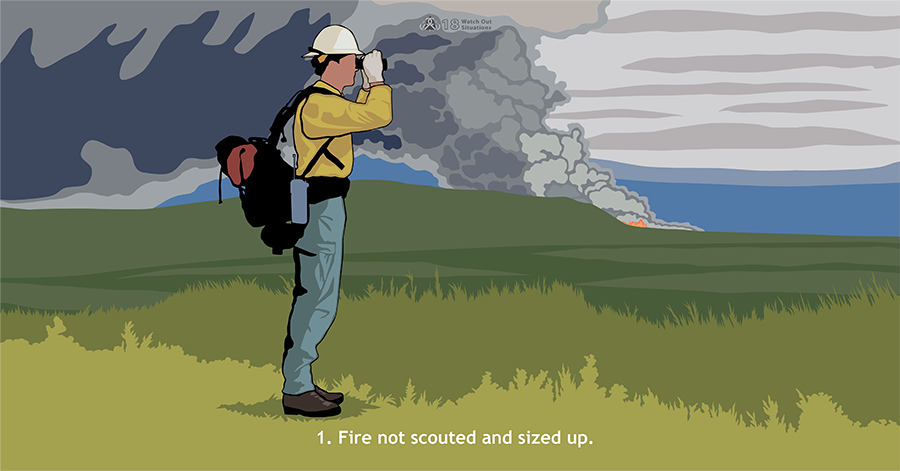
\includegraphics[width=0.49\textwidth, 
	trim={0cm 0cm 0cm 0cm}, 
	clip=true]
	{ops/pm118/118-01}
	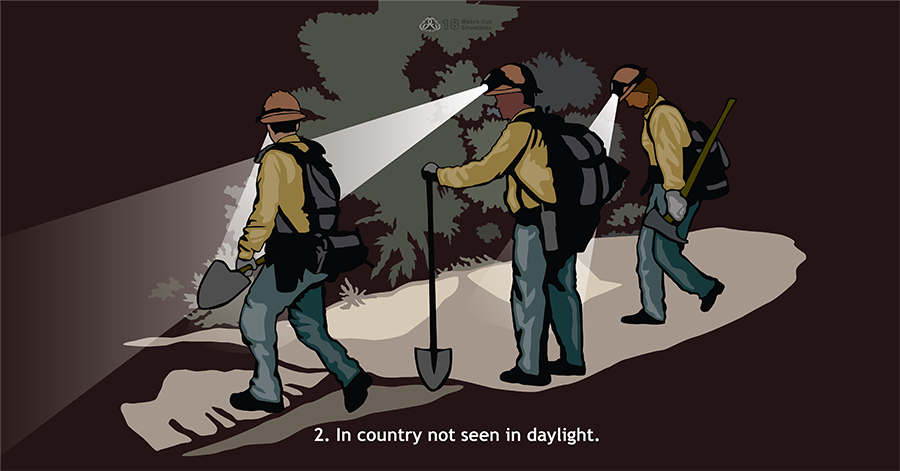
\includegraphics[width=0.49\textwidth, 
	trim={0cm 0cm 0cm 0cm}, 
	clip=true]
	{ops/pm118/118-02}  
	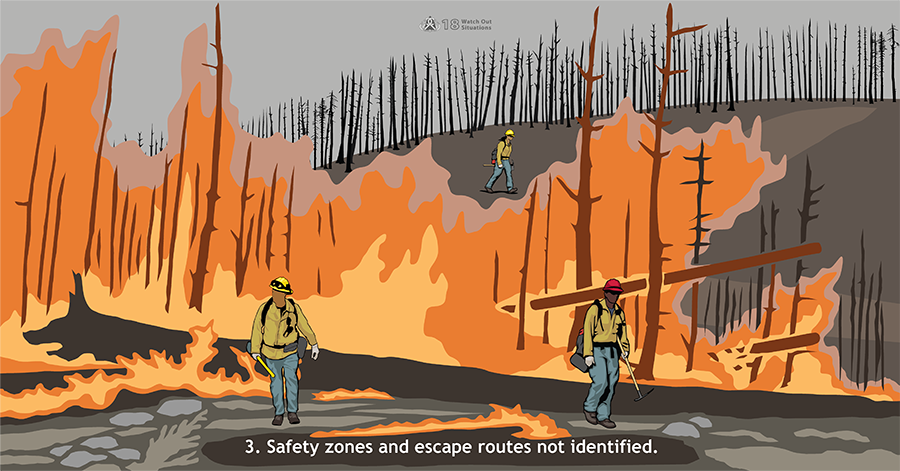
\includegraphics[width=0.49\textwidth, 
	trim={0cm 0cm 0cm 0cm}, 
	clip=true]
	{ops/pm118/118-03}
	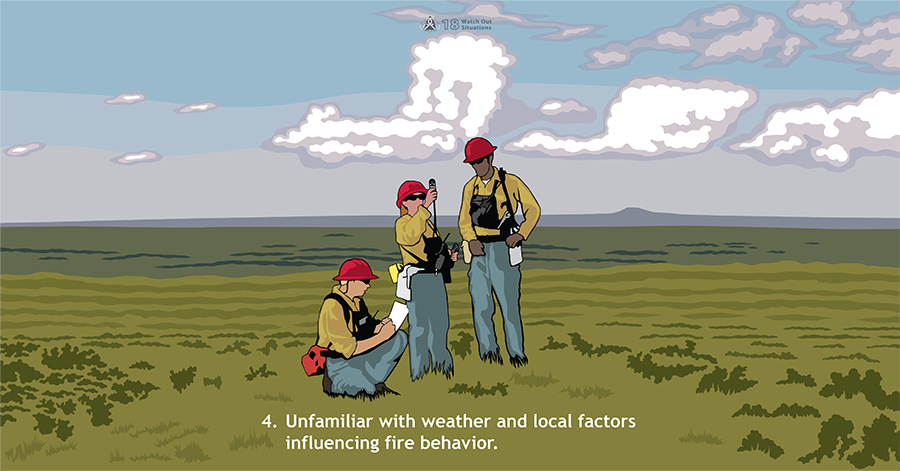
\includegraphics[width=0.49\textwidth, 
	trim={0cm 0cm 0cm 0cm}, 
	clip=true]
	{ops/pm118/118-04} 
		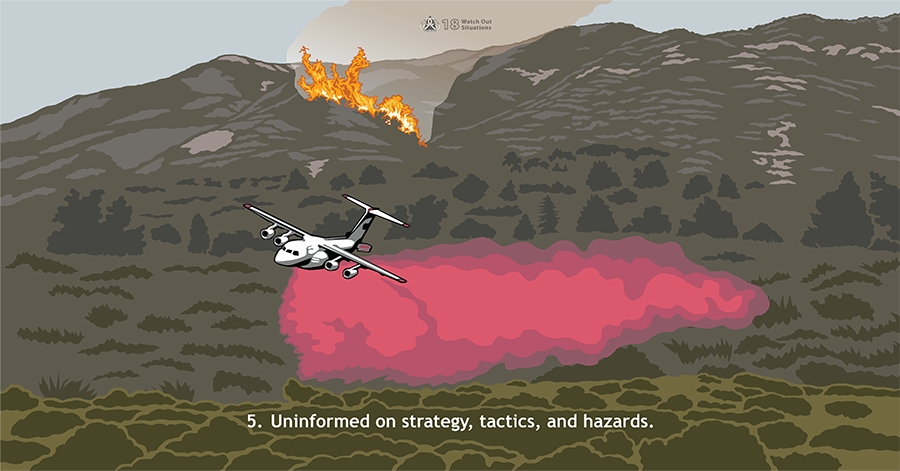
\includegraphics[width=0.49\textwidth, 
	trim={0cm 0cm 0cm 0cm}, 
	clip=true]
	{ops/pm118/118-05}
	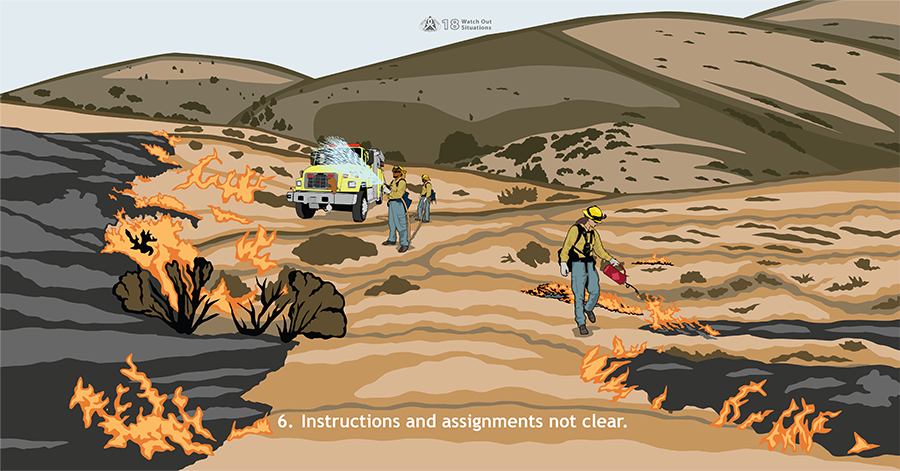
\includegraphics[width=0.49\textwidth, 
	trim={0cm 0cm 0cm 0cm}, 
	clip=true]
	{ops/pm118/118-06}  
	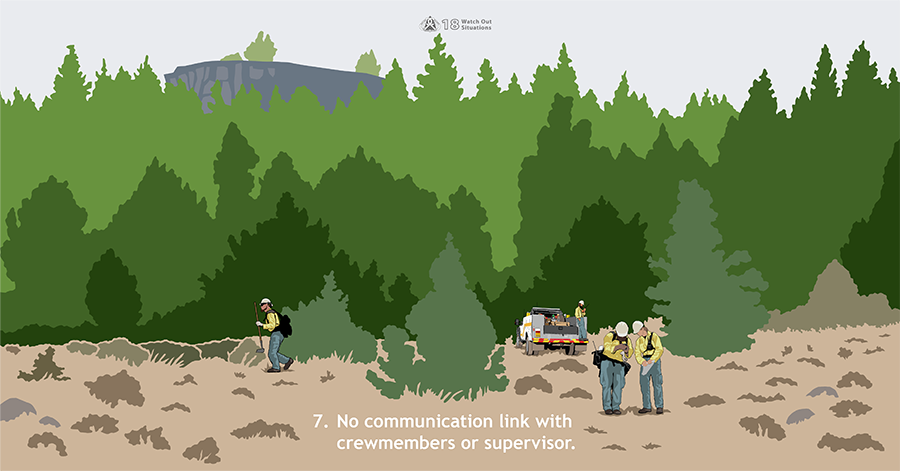
\includegraphics[width=0.49\textwidth, 
	trim={0cm 0cm 0cm 0cm}, 
	clip=true]
	{ops/pm118/118-07}
	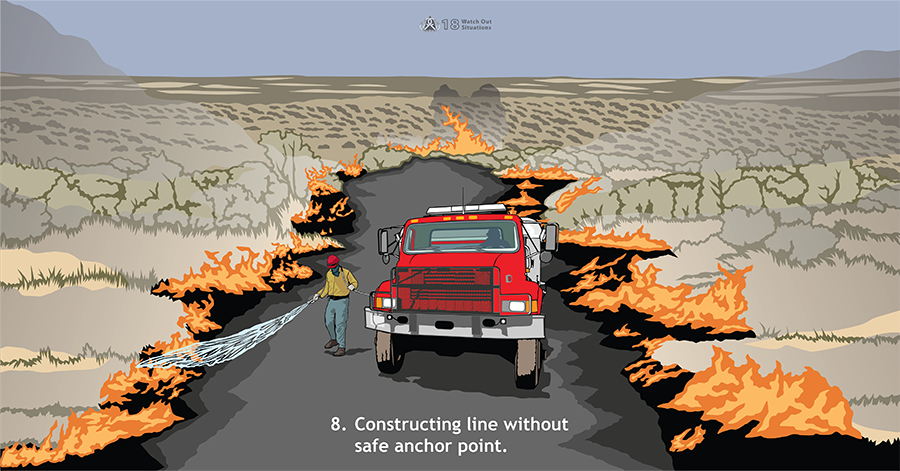
\includegraphics[width=0.49\textwidth, 
	trim={0cm 0cm 0cm 0cm}, 
	clip=true]
	{ops/pm118/118-08}  
		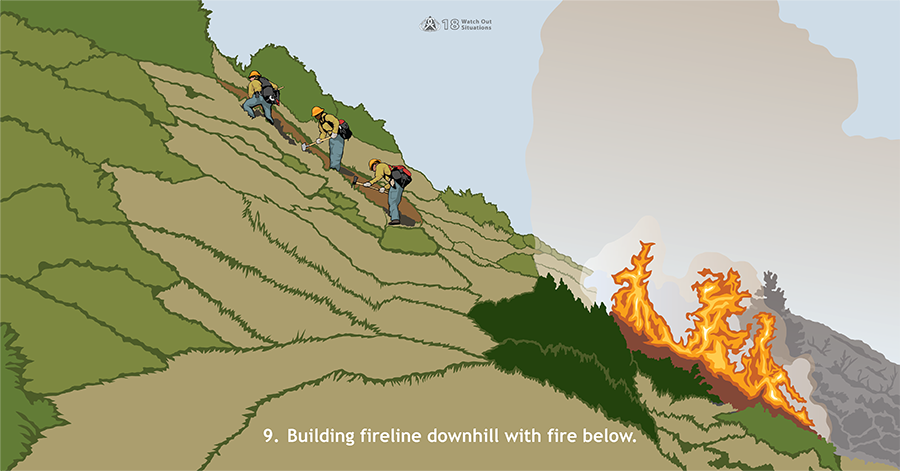
\includegraphics[width=0.49\textwidth, 
	trim={0cm 0cm 0cm 0cm}, 
	clip=true]
	{ops/pm118/118-09}
	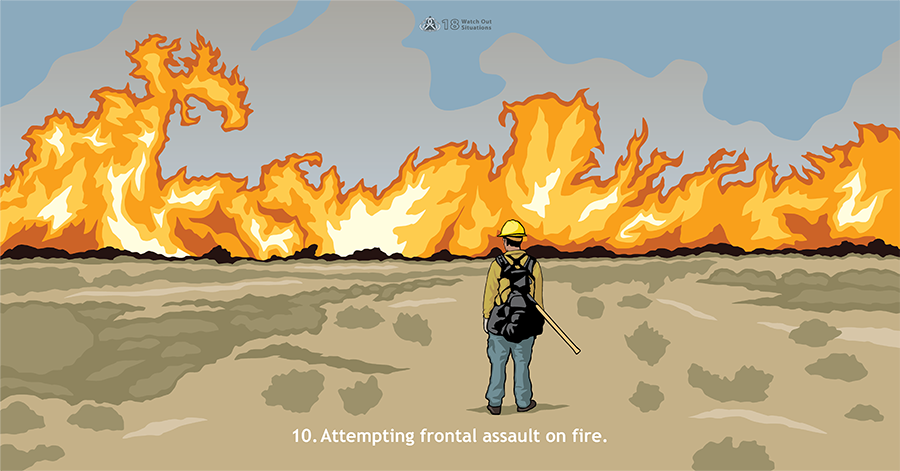
\includegraphics[width=0.49\textwidth, 
	trim={0cm 0cm 0cm 0cm}, 
	clip=true]
	{ops/pm118/118-10}  
\end{minipage}

\begin{minipage}{17cm}
	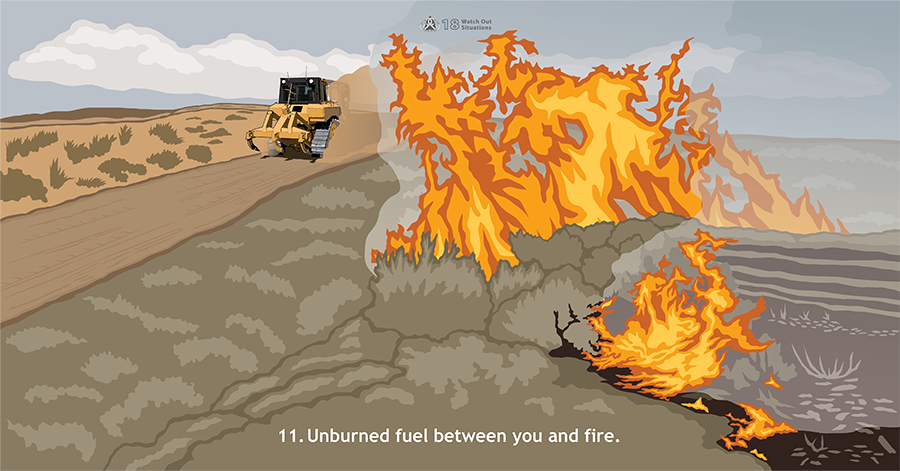
\includegraphics[width=0.49\textwidth, 
trim={0cm 0cm 0cm 0cm}, 
clip=true]
{ops/pm118/118-11}
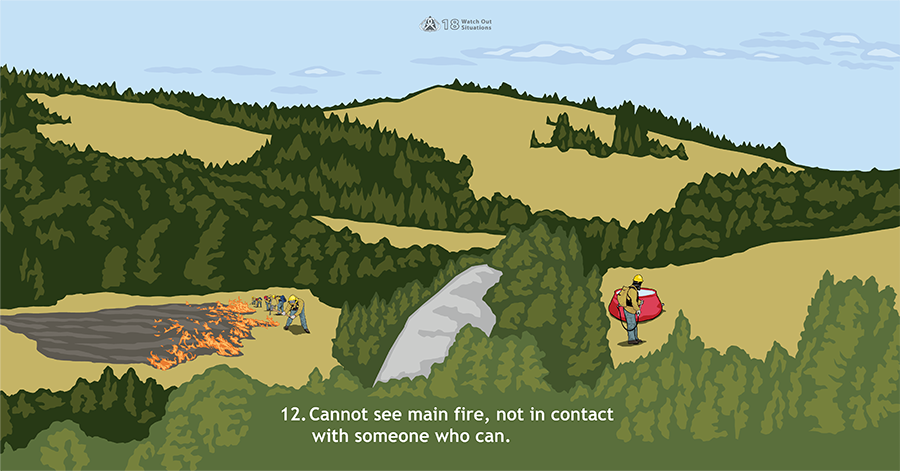
\includegraphics[width=0.49\textwidth, 
trim={0cm 0cm 0cm 0cm}, 
clip=true]
{ops/pm118/118-12} 
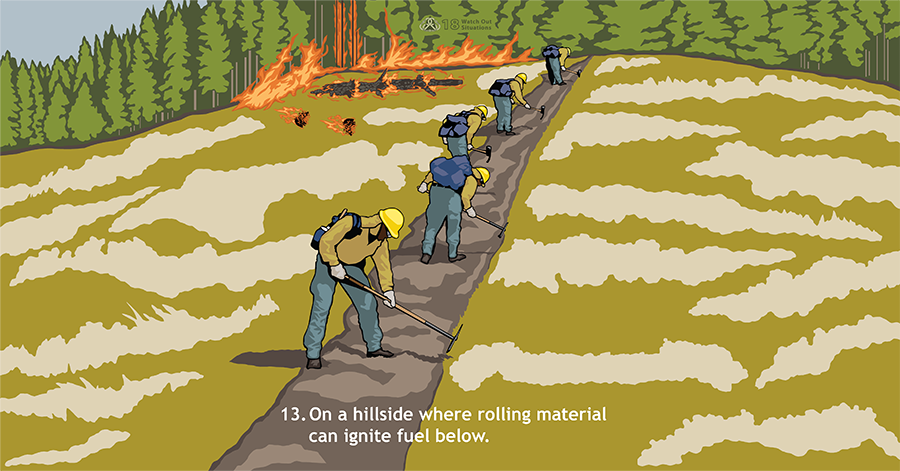
\includegraphics[width=0.49\textwidth, 
trim={0cm 0cm 0cm 0cm}, 
clip=true]
{ops/pm118/118-13}
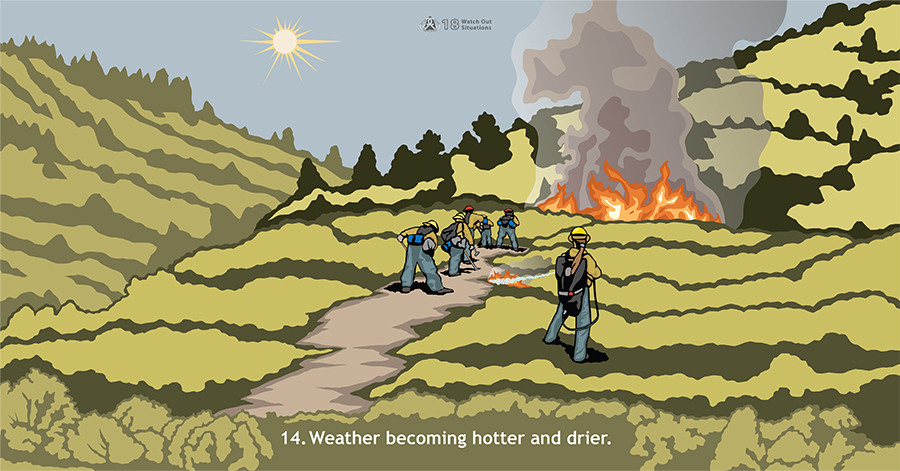
\includegraphics[width=0.49\textwidth, 
trim={0cm 0cm 0cm 0cm}, 
clip=true]
{ops/pm118/118-14}  
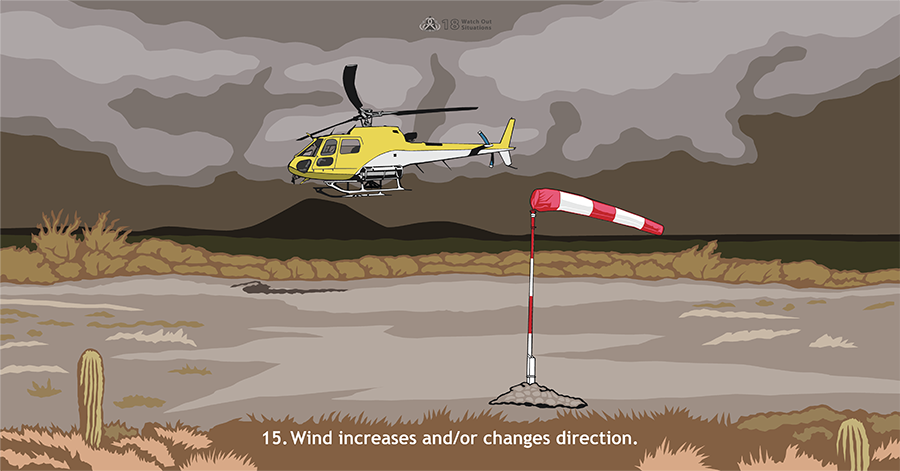
\includegraphics[width=0.49\textwidth, 
trim={0cm 0cm 0cm 0cm}, 
clip=true]
{ops/pm118/118-15}
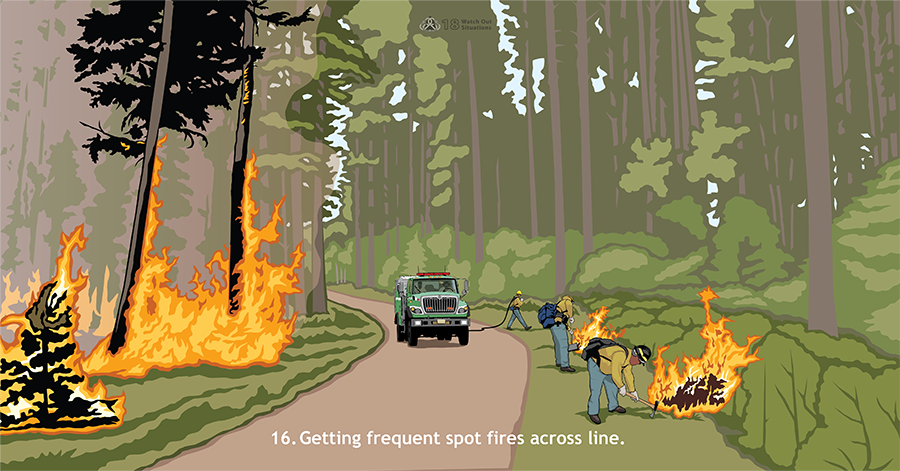
\includegraphics[width=0.49\textwidth, 
trim={0cm 0cm 0cm 0cm}, 
clip=true]
{ops/pm118/118-16} 
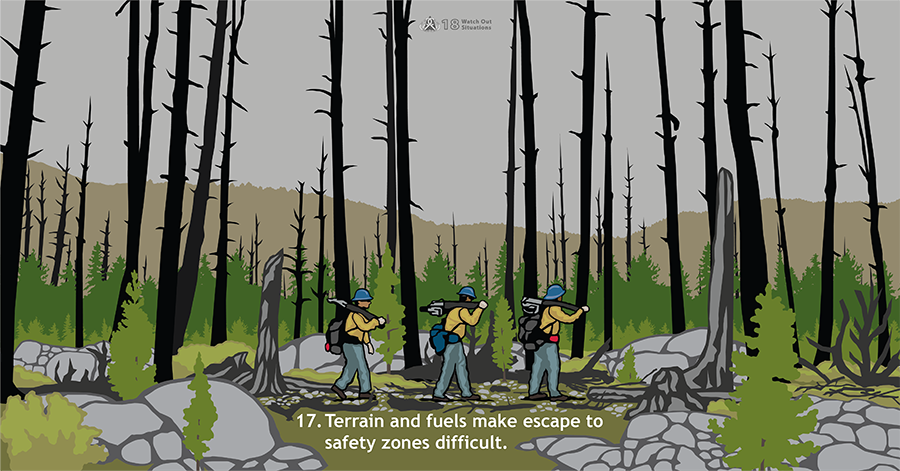
\includegraphics[width=0.49\textwidth, 
trim={0cm 0cm 0cm 0cm}, 
clip=true]
{ops/pm118/118-17}
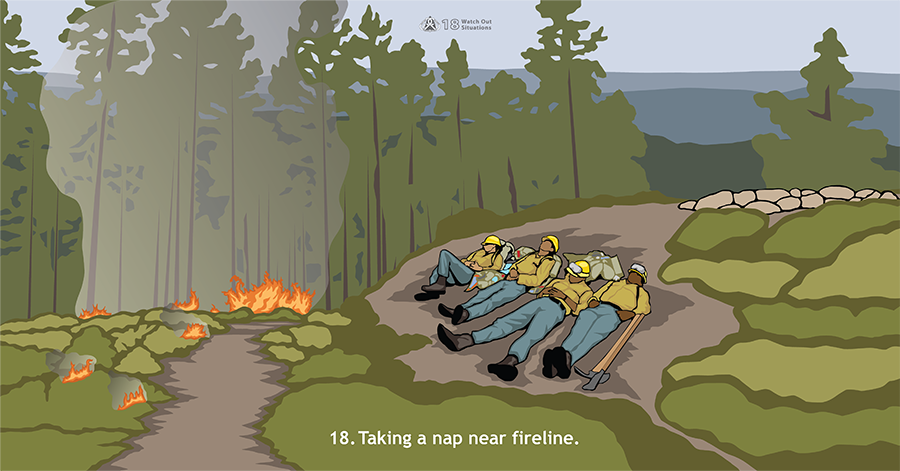
\includegraphics[width=0.49\textwidth, 
trim={0cm 0cm 0cm 0cm}, 
clip=true]
{ops/pm118/118-18}    

\end{minipage}

\section{Ten Standard Orders} 
\begin{minipage}{17cm}
	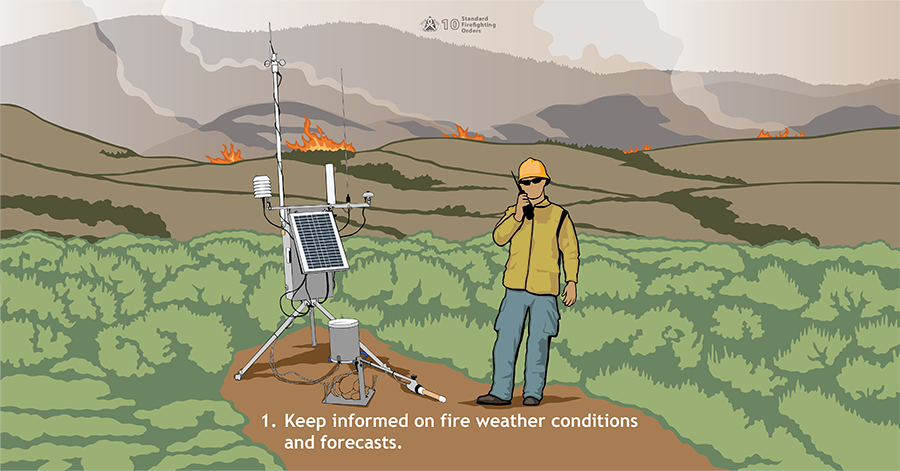
\includegraphics[width=0.49\textwidth, 
	trim={0cm 0cm 0cm 0cm}, 
	clip=true]
	{ops/pm110/110-01}
	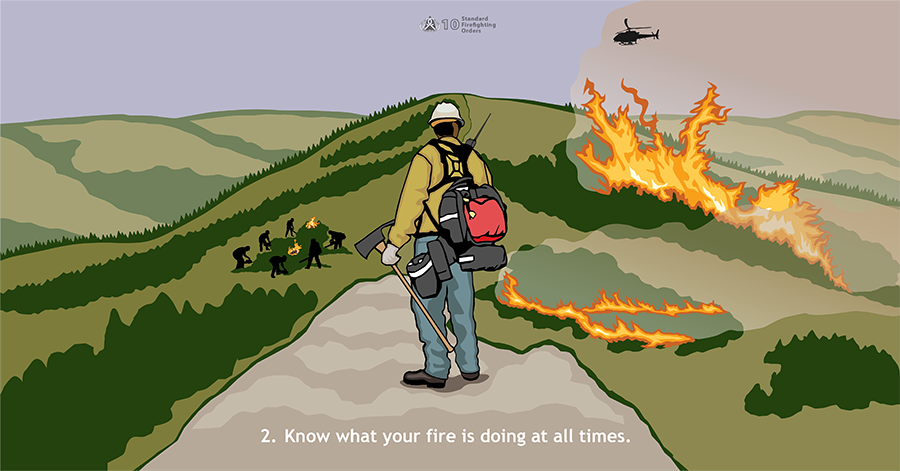
\includegraphics[width=0.49\textwidth, 
	trim={0cm 0cm 0cm 0cm}, 
	clip=true]
	{ops/pm110/110-02}	
	\includegraphics[width=0.49\textwidth, 
	trim={0cm 0cm 0cm 0cm}, 
	clip=true]
	{ops/pm110/110-03}
	\includegraphics[width=0.49\textwidth, 
	trim={0cm 0cm 0cm 0cm}, 
	clip=true]
	{ops/pm110/110-04}	
	\includegraphics[width=0.49\textwidth, 
	trim={0cm 0cm 0cm 0cm}, 
	clip=true]
	{ops/pm110/110-05}
	\includegraphics[width=0.49\textwidth, 
	trim={0cm 0cm 0cm 0cm}, 
	clip=true]
	{ops/pm110/110-06}	
	\includegraphics[width=0.49\textwidth, 
	trim={0cm 0cm 0cm 0cm}, 
	clip=true]
	{ops/pm110/110-07}
	\includegraphics[width=0.49\textwidth, 
	trim={0cm 0cm 0cm 0cm}, 
	clip=true]
	{ops/pm110/110-08}	
	\includegraphics[width=0.49\textwidth, 
	trim={0cm 0cm 0cm 0cm}, 
	clip=true]
	{ops/pm110/110-09}
	\includegraphics[width=0.49\textwidth, 
	trim={0cm 0cm 0cm 0cm}, 
	clip=true]
	{ops/pm110/110-10}
\end{minipage}



	
%\restoregeometry


\chapter{Holding}
\label{ch:holding}

Safe and effective prescribed fire begins with good \emph{control lines}\textemdash ``an inclusive term for all constructed or natural barriers and treated fire edges used to control a fire.\citep{nwcg2019}.'' \footnote{Managers (and this text) often use ``firebreak'', ``control line'', and ``fire line'' interchangeably, although this last term is more specific to line constructed for indirect attack of wildfire. }
While in wildfire suppression operations control lines are often hurriedly established in response to an ignition and anticipated direction of spread, prescribed fire managers have the advantage of defining the spatial extent of fire on their own terms. 

No control line can guarantee success on its own. 
But thoughtfully-placed and appropriately developed control lines provide a strong foundation to start fires with a high probability of remaining within the burn unit while affording managers good sight lines and accessibility. 

\section{Types of firebreaks}

\begin{figure}
	\begin{center}
		\includegraphics[width=0.45\textwidth]
		{ops/holding/DA0225}~
		\includegraphics[width=0.55\textwidth]
		{ops/holding/GravelRoadBreak} \\ 
		\includegraphics[width=0.47\textwidth]
		{ops/holding/HoldingEmberWatchOut}~
		\includegraphics[width=0.53\textwidth]
		{ops/holding/FlapperHolding}
	\end{center}
	\caption{Examples of readymade fire breaks.
		\emph{Top:} Existing roads make good firebreaks\textemdash typically wide, non-flammable, and accessible to equipment for ignition, holding, and suppression. 
		\emph{Bottom:} Two firefighters attend to fires from low-load, high-moisture vegetation conducive to containment. 
	} \label{fig:ReadyMadeBreaks}
	%(Fig.~\ref{fig:ReadyMadeBreaks})
\end{figure}

\subsection{Readymade breaks} 

 \begin{marginfigure}
	\begin{center}
		\includegraphics[width=2.2in]
		{ops/holding/ThorCreek}
		\caption{Sometimes it is best to just avoid the creek altogether.\label{fig:ThorCreek} } 
		% (Fig.~\ref{ThorCreek})
	\end{center}
\end{marginfigure} 

Existing roads make for excellent control lines (Fig.~\ref{fig:ReadyMadeBreaks}).
\emph{Slow fuel transitions} are another type of naturally-occurring or readymade fire break, defining the spatial threshold between flammable fuelbeds and low and/or green vegetation much less likely to carry fire (Fig.~\ref{fig:ReadyMadeBreaks}). 
Other areas of low flammability that can be incorporated into burn unit design include streams, rocky gulches, and outcroppings/ridges. 
When considering such features, it is important to consider both their tactical advantage\textemdash will a feature itself stop fire, or provide a good opportunity to burn out from with minimal preparation?\textemdash as well as their operational hazard\textemdash e.g., an uncrossable creek creates a level of complexity that managers can mitigate by putting line along the creek rather than across it (Fig.~\ref{fig:ThorCreek}). 

\subsection{Constructed line} 

\paragraph{Mineral lines}

The ideal line consists of \emph{mineral soil}\textemdash all vegetation is stripped away and the fire break is literally unable to burn such that no fire can creep across it.
In such cases, the degree of control provided by the line is limited only by its width\textemdash how long must flames be to lash across and ignite fuels outside the burn unit, and how long must embers smolder before they roll across and find receptive fuels. 

\begin{figure*} 
	\caption{\emph{Left \& center:} Wide mineral fire breaks constructed with farm tillage equipment make for robust control lines from which firing can be conducted with confidence.
		These lines in sw North Dakota were tilled through perennial grassland established on former crop fields (CRP), where damage to native sod and soil had already occurred.  
		\emph{Right:} In the Missouri Coteau, native prairie is often rocky, rolling, and invaded by the sod-forming Kentucky bluegrass, making for less reliable control lines that require frequent patrolling. 
	} \label{fig:MineralBreaks}
	\begin{center}
		\includegraphics[width=0.33\textwidth]
		{ops/holding/MineralBreak}~
		\includegraphics[width=0.33\textwidth]
		{ops/holding/WideMineralBreak2}~
		\includegraphics[width=0.33\textwidth]
		{ops/holding/SingleFurrow}
	\end{center}
	%(Fig.~\ref{fig:MineralBreaks})
\end{figure*}

Farm machinery is frequently implemented in constructing firebreaks for prescribed burns (Fig.~\ref{fig:MineralBreaks}). 
Generally speaking, tillage is more tenable on land currently or previously managed for agriculture\textemdash there is less concern about ``breaking virgin prairie''. 
Thus, wider lines that provide a high degree of control are possible when the terrain is conducive to wide tillage equipment (Fig.~\ref{fig:MineralBreaks}, \emph{left \& center}). 
But terrain and concerns about soil disturbance impact often limit mineral lines to a single furrow, which can be much more difficult to control, especially in vegetation types that form dense sod (Fig.~\ref{fig:MineralBreaks}, \emph{right}). 

\paragraph{Mowed fire breaks}

When tillage is not an option, mowing is a standard approach to creating lines of low fuels in which fire is much more easily controlled (Fig.~\ref{fig:MowedBreaks}). 
Rather than being non-combustible, mowed breaks are expected to burn to some degree, but fire is extinguished on the border of the unit as the black widens. 
Turning mowed lines cold is much more easily done when mowed vegetation is removed after cutting, which essentially creates a dense layer of fully-cured fine fuels. 
In many areas, frequent mowing tends to shift vegetation towards a generally less-flammable community dominated by sod-forming species. 
At the same time, these species also tend to be non-native; the ecological after-effects of fireline construction and maintenance must be considered alongside the ecological benefits of prescribed fire. 

\begin{figure} 
	\begin{center}
		\includegraphics[width=0.36\textwidth]
		{ops/holding/GreenMowedLine}~
		\includegraphics[width=0.64\textwidth]
		{ops/holding/MowedLineBreak}
	\end{center}
	\caption{When tillage to mineral soil is not an option, reducing fuel loads by mowing is a good option. 
		Mowed breaks are most effective when fuel removal is complemented by a slow-fuel transition, such as green, sod-forming grass along frequently-mowed trails (L). 
		Otherwise, fire can still spread through remaining dry stubble, although lower flame lengths facilitate control (R). 
		Note the undulating black line on the right, reflecting the fact that backing fires needed to be suppressed, and didn't go out on their own upon encountering lower fuel loads.   
	} \label{fig:MowedBreaks}
	%(Fig.~\ref{fig:MowedBreaks})
\end{figure}

\paragraph{Hand line}

When machinery is simply not an option, hand labor can create control lines. 
This is a conventional approach in indirect attack in wildfire suppression; hand crews dig narrow mineral lines from which ignitions specialists burn out to create wide control lines (Fig.~\ref{fig:Handlines}). 
Although it requires more physical effort than most prescribed fire managers prefer to exert for an extended period, hand line can be deployed to ``tie in'' gaps in fire breaks that machinery could not reach, or to create small defensible spaces within burn units (e.g., around power poles and structures). 
In woodlands and savannas where surface fuels are dominated by leaf litter, hand lines are easily constructed with rakes and leaf blowers (Fig.~\ref{fig:leaflines}). 

 \begin{marginfigure}[-4cm]
	\begin{center}
		\includegraphics[width=2.2in]
		{ops/holding/Rototiller}
		\\
	{Fortunately machinery has evolved since internal combustion engines were first applied to digging fire line. } 
		% (Fig.~\ref{fig:groundhog})
	\end{center}
\end{marginfigure}

\begin{figure} 
	\begin{center}
		\includegraphics[width=0.47\textwidth]
		{ops/holding/RxFireHandline}~
		\includegraphics[width=0.53\textwidth]
		{ops/holding/HandCrew}
	\end{center}
	\caption{When machinery can't reach locations that don't have usable natural fire breaks, crews with hand tools can attack the flame front directly (L) or support indirect attack by constructing line by hand (R). 
		The end goal is to remove vegetation down to mineral soil, often providing a point from which to begin backburning. 
	} \label{fig:Handlines}
	%(Fig.~\ref{fig:Handlines})
\end{figure}



\begin{figure} 
	\begin{center}
		\includegraphics[width=0.5\textwidth]
		{ops/holding/OakLeafBreak1}~
		\includegraphics[width=0.5\textwidth]
		{ops/holding/OakLeafBreak2}
	\end{center}
	\caption{These control lines in hardwood-dominated woodland outside Lawrence, Kansas were put in by the landowner with rakes and a leafblower.  
	} \label{fig:leaflines}
	%(Fig.~\ref{fig:leaflines})
\end{figure}

\section{Control tactics} 

It is essential that prescribed fire managers be prepared to control their fire. 
Crew members might need to take suppressive action in response to a spot fire or  \emph{slop over}\textemdash when fire manages to cross a control line and burn where it shouldn't\textemdash when the fire \emph{escapes}\textemdash i.e., begins to spread through a neighboring property not part of the burn unit\textemdash and simply when primary torch lines have served their purpose and no longer need to be burning at the edge of the unit. 

When flames are about 3 ft long or less, properly equipped and trained personnel  can attack directly using hand tools typical of a prescribed fire holding crew (e.g., flappers and rakes). 
Even then, fires ought to be engaged from control lines or the black. 
When flames are much longer than 3 ft, under no circumstances should anyone attack the fire directly with a hand tool. 
Such fires ought only to be engaged along the flanks, from the black, and with water\textemdash the radiant heat is just too intense to work near the fire even if wind is moving convective heat away. 

 \begin{marginfigure}
	\begin{center}
		\includegraphics[width=2.2in]
		{ops/holding/FlapperInSmoke}
		\caption{A holding crew member works to smother flames with a flapper. 
		\label{fig:flapper}  } 
		% (Fig.~\ref{fig:flapper})
	\end{center}
\end{marginfigure}

The primary objective of hand tools is to deprive a flame front of one or more sides of the flame triangle (Fig.~\ref{fig:FireTriangles}).  
For example, flappers are designed to smother the fire by denying oxygen to the reaction zone (hence the adage ``don't flap a flapper,'' which risks fanning the flames instead of smushing them out; Fig.~\ref{fig:flapper}). 
When properly used to reach ahead of the flame front and drag material back into the black, rakes remove fuel. 
In fine fuels, all of these interventions provide ample time for the reaction zone to cool, such that even if access to oxygen is restored, there is insufficient heat for combustion to occur. 







 
\chapter{Ignitions}
\label{ch:ignitions}


 \begin{marginfigure}[3cm]
	\begin{center}
		\includegraphics[width=2.2in]
		{ops/ignitions/DripTorchDiagram}
		\ImageCredit{Nebraska Prescribed Fire Council, via Facebook}
		\caption{Important components of the drip torch, with special reference to maintaining open grassland in the US Great Plains.
\label{fig:DripTorchDiagram} } 
		% (Fig.~\ref{fig:DripTorchDiagram})
	\end{center}
\end{marginfigure}

Most prescribed burns are deliberately started by humans with incendiary devices.%\footnote{Under the broader concept of \emph{wildland fire use} a prescription might also apply to a natural ignition in a wilderness area, allowing it to ``let burn'' under a specific set of conditions and/or within a specific area.} 
Tactically, these devices provide for the controlled firing of wildland fuels. 
Strategically, their operation can serve broad objectives such as fire behavior, fire effects, and smoke management. 
As such, wildland fire ignitions combine science and art. 

The most common firing device is the \emph{drip torch} (Fig.~\ref{fig:DripTorchDiagram}). 
While several configurations are available, each are essentially a handheld tank of liquid fuel with a wick that allows a small amount of fuel to pass over the burning wick, ignite, and carry fire to the fuelbed (Figs.~\ref{fig:IgnitionDevices}~\&~\ref{fig:FillingTorches}). 
Several other devices are basically extensions of the same principle\textemdash moving liquid fuel over a burning wick\textemdash and include vehicle-mounted torches with large-capacity tanks and fuel pumps for extended range (Fig.~\ref{fig:IgnitionDevices}, \emph{center}). 

Another major class of firing devices includes those that launch, propel, or release flares or fuel capsules containing a special mix of chemicals (e.g., potassium permanganate \& glycol) that, once combined, slowly undergo a reaction that eventually releases enough heat to ignite vegetation (Fig.~\ref{fig:IgnitionDevices}, \emph{right}). 
Capsules are launched via handheld devices or dropped from helicopters and drones.
Such devices enable remote ignitions, when physically standing in or near the fuel is difficult or hazardous. 



\begin{figure} 
	\begin{center}
		\includegraphics[width=1\textwidth]
		{ops/ignitions/IgnitionDevices}
		\ImageCredit{L: Noble Research Foundation, CC BY-NC-ND 2.0; C: Carissa Wonkka; R: Geoff Liesik, BLM, public domain}
		\ImageIndex{CC BY-NC-ND 2.0}
		{fig:SlingPsychrometer}
		{Noble Research Foundation}
		{https://www.flickr.com/photos/noblefoundation/6775182446}
	\end{center}
	\caption{L: The drip torch is the primary source of prescribed fire ignitions. C: ATV-mounted torches facilitate faster firing. 
	R: A pistol-style flare launcher fired by a member of the Wolf Creek Hotshots on the Bear Fire near Helper, Utah. 
	Such devices facilitate remote ignitions. 
	} \label{fig:IgnitionDevices}
	%(Fig.~\ref{fig:IgnitionDevices})
\end{figure}

\section{Ignition patterns} 

 \begin{marginfigure}
	\begin{center}
		\includegraphics[width=2.2in]
		{ops/ignitions/FillingTorches}
		% \ImageCredit{ }
		\caption{Drip torches are filled with liquid fuel, sometimes kerosene, but often a mix of 40\% gasoline and 60\% diesel fuel. 
			The gasoline provides rapid ignition at the wick, while oil in the diesel allows the fuel to burn long enough to transfer heat to vegetation.
			\label{fig:FillingTorches} } 
		% (Fig.~\ref{fig:FillingTorches})
	\end{center}
\end{marginfigure}

Perhaps the most determinant factor for prescribed fire effectiveness and operational safety is the way ignitions are applied to the burn unit, known as the \emph{ignition pattern}. 
Because wind is so important to fire intensity and spread, almost all ignition plans are made with reference to wind direction (Fig.~\ref{fig:IgnitionPatterns}). 
Topographic effects and potential impacts within and beyond the burn unit also influence the ignition pattern, such as which side of a unit is best to start firing from, and which direction(s) smoke must not be allowed to travel. 
Combining these two elements defines the acceptable wind directions for a given unit\textemdash some burn units might be so simple and hazard-free that they can be burned on days with wind coming from any direction, whereas some units have such a high degree of complexity that managers would only begin firing if the wind was from a specific direction.   

\begin{figure} 
	\begin{center}
		\includegraphics[width=1\textwidth]
		{ops/ignitions/IgnitionsMartinDell}
	\end{center}
	\caption{Six ignition patterns for prescribed fire \citep{martin1978}. 
		Numerals indicate order of firing. 
		The center fire pattern is often applied as a spiral, with a single ignition operator beginning in the center of the unit and circling out to the edges. 
		This facilitates, on the scale of the entire burn unit, the sort of convective ``pull'' illustrated below. 
	 \label{fig:IgnitionPatterns} }
	%(Fig.~\ref{fig:IgnitionPatterns})
\end{figure}

Within the unit, the pattern of ignition is generally chosen based on desired fire effects and limitations on spread. 
Broadly speaking, patterns facilitate (a) faster, more intense head fires that move with the wind; (b) slower-moving backing fires that might have longer residence time as they creep against the wind; or (c) a series of flanking fires that spread perpendicularly to the wind and combine behavior and heating properties of both head and backing fires (Fig.~\ref{fig:IgnitionPatterns}). 
The number and spacing of strips and spots can be varied to regulate the direction and amount of smoke emissions and the time it takes to completely burn the unit.

\begin{marginfigure} 
	\begin{center}
		\includegraphics[width=2.2in]
		{ops/ignitions/PrimaryTorchLine}
	\end{center}
	\caption{A primary torch operator starts a back burn from right along the fire break, which in this case is a two-track road with gravel and low vegetation accessible by pumper vehicles for holding the fire within the unit. 
	 \label{fig:PrimaryTorch} }
	%(Fig.~\ref{fig:PrimaryTorch})
\end{marginfigure}

Almost every ignition pattern begins with a line of fire placed perpendicular to the wind on the downwind side of the unit (Fig.~\ref{fig:IgnitionPatterns}). 
Because the wind is pushing this fire away from the area intended to be burned line is typically ran along a robust fire break that combines (a) low or no fuels beyond the edge of the burn unit with (b) accessibility to vehicles that can suppress fire and patrol the line (Fig.~\ref{fig:PrimaryTorch}). 

\begin{figure}[t] 
	\begin{center}
		\includegraphics[width=0.465\textwidth]
		{ops/ignitions/WonkkaStrips}~
		\includegraphics[width=0.535\textwidth]
		{ops/ignitions/SecondaryTorchWoods}
	\end{center}
	\caption{\emph{Left:} Dr. Carissa Wonkka lays a strip head fire through a grassland fuelbed to both widen the ``black'' downwind but also lift the smoke column off the control lines to make live better for holding crew. 
		\emph{Right:} A secondary torch operator lays a strip inside of the primary operator, who is firing off the road. 
		An engine supports holding behind the torches as they move forward. 
		\label{fig:SecondaryTorch} }
	%(Fig.~\ref{fig:SecondaryTorch})
\end{figure}

\begin{marginfigure} 
	\begin{center}
		\includegraphics[width=2.2in]
		{ops/ignitions/RothermelSecondary}
			\ImageCredit{\citet{rothermel1984}}
	\end{center}
	\caption{Under good convective conditions, two parallel strip fires will interact.
		The primary line, burning more intensely as it has been burning longer, will ``pull'' the secondary line in towards it, which enhances control by limiting the outward rate of spread. 
		Meanwhile, the secondary line will draw the convective column into the unit, allowing smoke to ventilate more vertically and keep it above crewmembers working on the line.   
		\label{fig:rothermel1984} }
	%(Fig.~\ref{fig:rothermel1984})
\end{marginfigure}

As the burn crew works to develop control lines around the entire burn unit\textemdash widening fire breaks with burned-out areas to increase the distance between flames and embers from the unit and fuels beyond the edges of the unit\textemdash additional torch operators are often deployed within the burn unit (Fig.~\ref{fig:SecondaryTorch}). 
These secondary torch operators lay \emph{strip ignitions} that not only increase the burned area by widening the lines faster, but under good convective conditions actually influence the interaction between the prescribed fire and the atmosphere (Fig.~\ref{fig:rothermel1984}). 

Under very good convective conditions, the smoke columns of distant flame fronts will interact in the atmosphere (Fig.~\ref{fig:PlumesConverge}). 
These interactions can temporarily change the direction and rate of spread, reducing the relative influence of wind. 
At very broad scales, such as large wildfires, the driver of spread rate and direction can shift from wind to convention, creating a \emph{plume-driven fire}. 

\begin{figure}[b]
	\begin{center}
		\includegraphics[width=1\textwidth]
		{ops/ignitions/PlumesConverge}
		\ImageCredit{Austin Catlin, BLM, public domain}
	\end{center}
	\caption{A remarkable image of two plumes converging on the Market Lake Prescribed Fire in eastern Idaho.
	The lighter smoke is from light fuels (e.g., grass) that fully combusted. 
	The darker smoke is due to heavier fuels pulled aloft prior to complete combustion and/or combustion of secondary compounds in the vegetation (e.g., sagebrush). 
	} \label{fig:PlumesConverge}
	%(Fig.~\ref{fig:PlumesConverge})
\end{figure} 

 %\chapter{Pumps and engines} 

%\addcontentsline{toc}{chapter}{Bibliography}
%
%	Call the bibliography
%
\clearpage
\begin{fullwidth} % Makes the refs go all the way across page
\bibliographystyle{elsarticle-harv} 
\bibliography{FireScienceWorkshop.bib}
\clearpage 
\part{Worksheets} 
	% include the taskbook
\addcontentsline{toc}{chapter}{Taskbook}
	\includepdf[pages={1-},scale=1]{sections/worksheets/Taskbook.pdf}
% include 5 copies of the scouting report
\addcontentsline{toc}{chapter}{Scouting report}
	\includepdf[pages={1-},scale=1]{sections/worksheets/ScoutingReport.pdf}
	\includepdf[pages={1-},scale=1]{sections/worksheets/ScoutingReport.pdf}
	\includepdf[pages={1-},scale=1]{sections/worksheets/ScoutingReport.pdf}
	\includepdf[pages={1-},scale=1]{sections/worksheets/ScoutingReport.pdf}
	\includepdf[pages={1-},scale=1]{sections/worksheets/ScoutingReport.pdf}
% include 5 copies of the briefing mad lib
\addcontentsline{toc}{chapter}{Briefing mad lib}
	\includepdf[pages={1-},scale=1]{sections/worksheets/BriefingMadLib.pdf}
	\includepdf[pages={1-},scale=1]{sections/worksheets/BriefingMadLib.pdf}
	\includepdf[pages={1-},scale=1]{sections/worksheets/BriefingMadLib.pdf}
	\includepdf[pages={1-},scale=1]{sections/worksheets/BriefingMadLib.pdf}
	\includepdf[pages={1-},scale=1]{sections/worksheets/BriefingMadLib.pdf}
% include 1 copy of the fire behavior sampling protocol
	\addcontentsline{toc}{chapter}{Thermocouple deployment protocol}
	\includepdf[pages={1-},scale=1]{sections/worksheets/ThermocoupleDeploymentProtocol.pdf}
% include 1 copy of the fuel sampling protocol
\addcontentsline{toc}{chapter}{Fuel sampling}
	\includepdf[pages={1-},scale=1]{sections/worksheets/FuelSamplingProtocol.pdf}
% include 5 copies of the fuel sampling datasheet
	\includepdf[pages={1-},scale=1]{sections/worksheets/FuelsDatasheet.pdf}
	\includepdf[pages={1-},scale=1]{sections/worksheets/FuelsDatasheet.pdf}
	\includepdf[pages={1-},scale=1]{sections/worksheets/FuelsDatasheet.pdf}
	\includepdf[pages={1-},scale=1]{sections/worksheets/FuelsDatasheet.pdf}
	\includepdf[pages={1-},scale=1]{sections/worksheets/FuelsDatasheet.pdf}
% include 1 copy of the fire behavior modeling exercise
\chapter{Fire behavior modeling exercise}

The following pages reproduce the necessary pages from the NWCG Fireline Appendix B to complete a Fire Behavior Worksheet (p. B-5) for Grass Fuel Model 1 or 2, on a given set of input parameters either measured or hypothetical for the purpose of the example (dry bulb temperature, relative humidity, wind speed, slope, aspect, fuel shading, etc). 
Although Appendix B Output tables for FM 1-3 are included, nomograms for both low and high windspeeds from \citet{rothermel1983} for FM 1 and 2 are also included. 
\newpage 

\includepdf[pages={1-},scale=1]{sections/worksheets/ExampleAppendixB.pdf}
\includepdf[pages={1-},scale=1]{sections/worksheets/ExampleNomograms.pdf}
	 
\end{fullwidth}
%
\end{document}